\documentclass[12pt]{report}
\usepackage{./Style/gscale_thesis}
\usepackage{./Style/fancyheadings}
\usepackage{./Style/natbib} %bibliography style for books and articles
\usepackage{./Style/setspace}
\title{FIXME: Memoirs of a Code Plumber}
\halftitle{FIXME}

\author{Gabriel Dalimonte}
\shortauthor{G. Dalimonte}

\dept{Computing \& Software}
\field{Software Engineering}

\prevdegreeone{B.Eng. (Software Engineering \& Game Design),\\ McMaster University, Hamilton, Canada}

\prevdegreetwo{B.Eng.}

\submitdate{October 2019}

\copyrightyear{2019}

\principaladviser{Dr. Jacques Carette}

\setcounter{tocdepth}{1}

% Additional packages
\usepackage{graphicx}
\usepackage{subcaption}
\usepackage[justification=centering]{caption}
\usepackage[hidelinks,bookmarksdepth=3]{hyperref}
\usepackage{array}
\newcolumntype{P}[1]{>{\raggedright\let\newline\\\arraybackslash\hspace{0pt}}m{#1}}
\usepackage{booktabs}
\usepackage{longtable}
\usepackage{float}
\usepackage{enumerate}
\usepackage[shortlabels]{enumitem}
\usepackage[shortcuts]{extdash}
\usepackage{amsmath}
\usepackage{amsfonts}
\usepackage{multirow}
\usepackage{hyperref}
\usepackage{listings}
\usepackage{framed}
\usepackage[chapter]{minted}
\usepackage{tcolorbox}
\tcbuselibrary{breakable}
\usepackage{multicol}
\usepackage{tabularx}
\usepackage{environ}

\lstset{frame=single}
\newenvironment{longlisting}{\captionsetup{type=listing}}{}  % Literal theft from: https://tex.stackexchange.com/a/368971
\providecommand*{\listingautorefname}{Listing} % https://tex.stackexchange.com/questions/13760/use-autoref-with-minted-and-its-listing-environment
\renewcommand*{\chapterautorefname}{Chapter}
\renewcommand*{\sectionautorefname}{Section}
\renewcommand*{\subsectionautorefname}{Subsection}
\setmintedinline{breaklines}
\newmintinline[haskell]{haskell}{}
\newmintinline[makefile]{makefile}{}
\newmintinline[bash]{bash}{}
\newcommand{\CC}{C\nolinebreak\hspace{-.05em}\raisebox{.4ex}{\tiny\bf +}\nolinebreak\hspace{-.10em}\raisebox{.4ex}{\tiny\bf +}}
\def\CClb{C\raise.22ex\hbox{{\footnotesize +}}\raise.22ex\hbox{\footnotesize +}}

\graphicspath{{Images/}}

% ********************************
\begin{document}                     
	\beforepreface
	\prefacesection{Executive Summary}\label{execSum}

This report investigates the design and use of the Drasil software framework, which uses knowledge capture to facilitate automation of scientific computing software creation. Drasil is developed in a collaborative setting amongst several developers with range of backgrounds and experience. Contributing to a collaborative codebase poses many challenges, from the unfamiliarity of code layout, to the overarching design, to the myriad of preexisting undocumented choices. With Drasil's design being driven on an as-needed basis, it can be hard to discern whether an odd design is intentional and relevant, historical, or ad-hoc. Drasil's ad-hoc development process leads to designs lack foresight leading to designs that are difficult to extend.

We inspect several odd Drasil designs from the dual perspective of a developer and user of Drasil. We uncover several design oddities stemming from the just-in-time nature of Drasil's development. Many of the faults appear shallow at first glance; however, they have a cascading effect requiring large swathes of changes to address. We inspect \textit{how} an odd constructor propagates throughout the Drasil codebase to discover that, while each individual component is designed appropriately, the macro-level design is incoherent and requires development attention. Discovered design faults, related to consistency, coalesced, seeing resolution through an introspective data-structure, used to ensure the consistency of all sections in a requirements document.

Aside from investigating design faults, this report looks for automation candidates, considering both perspectives. From the user-facing perspective we identify nonsensical incantations required for otherwise automated sections of a requirements document. We improve the user experience by removing the unnecessary incantations while maintaining, and abstracting, the function the boilerplate performed. We realize developer automation improvements by through convenience of the build system, the number and depth of tests the continuous integration process performs, automating and improving select forms of feedback for developers, and automatically producing an up-to-date demonstration website of Drasil and its capabilities whenever a change occurs.

Even a reasonable design, or minor fault, is worth investigating in depth. The investigation may reveal additional faults, or design oversights, before they compound to a point of untenable technical debt.
	\referencepages
	\afterpreface
	
	\chapter{Introduction}\label{intro}
%\section{Problem}\label{iproblem}
% Why does Drasil exist?
% 	What is it?
Scientific Computing (SC) is a diverse domain of software development focused on using computers to aid in solving science and engineering problems. Mathematical models and algorithms are designed and implemented to calculate various properties about the modeled real-world systems, such as maximum load and failure rate. Some examples of scientific software are modeling the physics for a bridge, protein folding, and an algorithm for an ordinary differential equation solver.

Due to the important nature of SC software, SC focuses on correctness, consistency, and traceability, among other properties, to ensure high-quality software. In an effort to design software following the listed properties, SC software should include other deliverables besides the code implementation, such as a test plan to ensure the software's behaviour.

% 	Time
Ensuring the quality of (SC) software can be a time-intensive effort. Constructing all required -- or desired -- documentation, such as a high-level design document and test plan, can greatly increase the amount of work required. Any inconsistency found in any deliverable will require a reexamination of all deliverables to ensure the mistake did not propagate elsewhere. For example, a sign error in a requirements document may propagate into the code implementation and not be discovered until testing occurs. 

% 	Certification
Some scientific software, such as those that are involved in power generation, or are otherwise safety relevant, must pass a certification process prior to being used in real-world situations. Certification is an extensive process necessitating a requirements document, a high-level design document, the complete source code for the software, a test plan, and the testing results, to name some possible deliverables. Due to the rigor involved with software certification, it is an expensive process. Small inconsistencies between --- or within --- any of the provided items can result in a rejection. It becomes imperative for a software product and associated documentation to be pristine before entering the certification process.

Certified software rarely sees modification post-certification. Any software modifications tend to require a complete recertification of the system because the system-wide impact of an alteration is unknown. Due to the cost of applying for certification again, the time to proofread the existing documentation to ensure they maintain consistency in the modified version, and the scale of changes to the existing software, it does not make financial sense in many situations to attempt recertification. 

\section{Drasil}\label{idrasil}
% Introduce Drasil
To combat the difficulties of producing high-quality SC software, we look to Drasil~\cite{GitRepo}\cite{SzymczakEtAl2016}. Drasil is a framework of embedded domain-specific languages (eDSLs) used to \textit{describe} a software system. From the description of a software system, Drasil generates a requirements document, implementation code in four different imperative-style languages (\CC, C\#, Java, Python), and Doxygen comments for the generated code. All of the artefacts are derived from a single description of a software system. Drasil aims to be modular by-design to allow users to implement additional artefact types and document formats without requiring comprehensive changes to the core language.

Drasil addresses the difficulties of producing consistent SC software through the use of a single structure (\haskell{SystemInformation}) that provides a description of a software system. By only specifying information once, any documents generated must be consistent by-construction. Further, a change to the description will update all artefacts appropriately, reducing the burden incurred by modification. Due to Drasil's centralised knowledge, tasks that are tedious for humans, like constructing a table showing dependencies of requirements on assumptions, can be performed automatically during artefact generation. Through the process of ``faking" the rational design process~\cite{parnas1986rational}, Drasil reduces the tedious bookkeeping-type work required for certification through its artefact generation process.

% Example of reuse
\autoref{lst:iglassbr} contains a brief piece of code describing the name, or \textit{idea}, of a software system bundled with and elaborated in Drasil, named ``GlassBR." A \textit{commonIdea}, or \haskell{CI}, encodes the concept of a noun for use with Drasil. The first \\

\begin{listing}[H]
\begin{tcolorbox}
\begin{minted}{haskell}
glassBR :: CI
glassBR = commonIdeaWithDict "glassBR" (pn "GlassBR")
  "GlassBR" [idglass]
\end{minted}
\end{tcolorbox}
\caption{A Drasil \textit{chunk} representing the \textit{idea} of a software system ``GlassBR."}
\label{lst:iglassbr}
\end{listing}

\noindent argument applied to \haskell{commonIdeaWithDict} specifies a unique identifier, which is used internally within Drasil to perform database lookups during artefact construction. In the case of \haskell{glassBR}, the string \haskell{"GlassBR"} is a proper noun and specified as such using the \haskell{pn} smart constructor, comprising the second argument, or \textit{what} the idea is and the semantics related to displaying it. The third argument may be an abbreviation, or acronym, of the idea. The final argument is a list of domains that the idea belongs to for information categorisation purposes. The particular definition displayed in \autoref{lst:iglassbr} is further used to specify the name of generated software system. The GlassBR example bundled with Drasil generates a Software Requirements Specification (SRS) and implementation code for the system. Of the artefacts generated ---\ \LaTeX\ SRS, HTML SRS, \CC~implementation, C\# implementation, Java implementation, and Python implementation --- the \haskell{glassBR} definition specified above is responsible for 50 appearances of the string. Each SRS contains 18 instances of the phrase ``GlassBR," while the remaining 14 locations of the noun occur in the generated code; the Java implementation uses the idea to place all generated code inside the ``GlassBR" package accounting for nine instances, while the remaining five appear in generated Doxygen configurations. With Drasil, renaming software system is a trivial task requiring only one line of modification! Modifying the line in \autoref{lst:iglassbr} is more straightforward and predictable than manually attempting a ``find and replace" across many artefacts in many languages, and hoping for the best.
% Note: GlassBR numbers are those ignoring the Makefile (which didn't exist before I added them including the Doxygen targets, althrough we do include the doxygen numbers)


% How further reuse gives us drasil-data and software families.
Drasil's reusability facilities can be used beyond a single software product. Information, like that specified in \autoref{lst:iglassbr}, may be reused in other software products to form \textit{software families}. A software family is a related set of software products with design parameters modified. Drasil contains a software family as two related examples: one is a Solar Water Heating System (SWHS), which involves a Phase Change Material (PCM), the other is a modification of SWHS to remove the PCM, named ``NoPCM." NoPCM reuses large portions of SWHS --- such as the requirements, assumptions, and models --- by sharing constructs between both examples. ``Common" knowledge may be further refactored into \textit{drasil-data}, a sub-package of Drasil that contains common domain-specific concepts, such as the mathematical constant $\pi$ and Newton's Second Law of Motion as a physics concept.
% FIXME: Should I cite these two examples (and if so caseStudies, Drasil code or generated artefacts), GlassBR, and Newton's 2nd?

% Problems with Drasil
\section{Shortcomings}\label{iprobdrasil}
% DL (SRSDecl)
Drasil's emphasis on reuse provides an excellent basis to dissect and discern what knowledge is required to properly design and specify a software system. Unfortunately, some of Drasil's earliest efforts were focused on simply encoding information to display in a certain way within an SRS rather than to properly capture knowledge that is sufficiently described to be reusable. The result of the ad-hoc design is display-oriented facilities that do not provide the correct level of abstract encoding to reuse the information outside of a requirements document. Such design-oriented information does not truly embody the idea of reuse that Drasil strives to achieve, where knowledge may permeate all artefacts of a system described.

% CI, DL (Multiplate)
Due to the ad-hoc design, Drasil includes substandard code as the result of substandard design decisions, which ironically violates Drasil's own design goal for reuse. Early additions to Drasil based on existing features tended to be implemented using copy-paste rather than integrating and considering the new feature with the existing codebase. The result is swathes of duplicated code that vary in few situations and requires a higher maintenance effort to enact the same change across multiple pieces of copy-pasted code.

% DL
Further stemming from the ad-hoc design of early Drasil is a lack of consistency within sub-packages of the project. Part of early Drasil was heavy experimentation with language constructs and the way ideas were exposed to users. Sometimes an experimental change would be made to one facility and left that way without any further modifications. These modifications may have improved the language in terms of reusability or ease-of-use, however, complicated internal design by requiring multiple methods to interact with similar data. In one particular case, the implicit passing of data through a more general data structure was a desirable change, although only applied to one constructor. The other constructors duplicated data already available in a common database; thus, forcing authors to specify the same information twice while allowing room for error. The unique data constructor that retrieved the data required from the database was typically ignored while designing systems that interacted with it, resulting in last-minute hacks to ``make it work," forming a feedback loop of hacks. The feedback loop of hacks reached a point where the technical debt was too high and it became reasonably difficult to include items associated with the anomalous constructor in some derived data. The derived data simply omitted information ``belonging" to the anomalous constructor.

% DL (Traceability, others), BS
% FIXME: Next two paragraphs need another pass.
Much of the developmental effort for Drasil has been focused on improving what is generated. An oft ignored aspect of Drasil's development is the ease-of-use when attempting to encode knowledge in Drasil as well as the (in)convenience to describe artefacts and how they should use available information. A user would notice, when producing an example from scratch, the odd incantations needed to make certain pieces of artefact generation work correctly. When improvements are made to document generation, which displays information automatically derived from user-specified knowledge, the layout of the new information is not always a concern and seen as something to revisit. The deferral of correcting the layout and how the information is displayed leaves Drasil producing unappealing sections of documents, which are hard to read or interpret.

% BS cont
The build system of Drasil is ad-hoc and lacks developer attention as it does not immediately improve the artefacts generated. The build system for Drasil provides the bare minimum required to build the sub-packages and lightly test the artefacts generated by Drasil. Building any artefacts Drasil generates is a tedious process for a human, resulting in many instances where developers make changes that break the correctness of artefacts Drasil produces.

% Overview of What I Did
\section{Problems Addressed}\label{iplan}
With the shortcomings of Drasil in mind, \autoref{ci} examines a seemingly small issue encountered in \autoref{toyexample}. Through examining how the associated data is passed between sub-packages and functions, we discover a larger design problem resulting from an ad-hoc, early Drasil implementation. We conclude by unifying several related pieces of code and data structures, anticipating future development, in an attempt to reduce maintenance effort. \autoref{dl} addresses an inconsistent (but better) abandoned, experimental design that added an unexpected hurdle in the implementation of \autoref{ci}. During the course of addressing the hurdle, \autoref{dl} examines a wide range of boilerplate and awkward design, remediating each to realize a better design, more aligned with Drasil's design philosophies. Finally, \autoref{bs} begins by examining how to automate the tedious, repetitive, Drasil developer action of compiling the\ \LaTeX\ and generated code for the bundled examples. The task escalates in \autoref{contInt} producing a better testing process for potential changes to Drasil to improve code quality and consistency while reusing the generated artefacts to demonstrate the project to prospective users interested in Drasil. The end result of \autoref{contInt} is a test suite that analyses the Drasil codebase statically, the generated artefacts, and produces an archive of artefacts readily accessible online.

		\setcounter{figure}{0}
		\setcounter{equation}{0}
		\setcounter{table}{0}
	\chapter{Details of Drasil}\label{toyexample}

Drasil is a complex system involving a number of sub-packages, which can be combined in ways to produce a number of artefacts. Understanding the intricacies of the language and systems can be a daunting task. In an effort to acclimate the reader to Drasil as a system and a language, we present two views of Drasil. \autoref{teHow} examines Drasil at the sub-package level, describing briefly what each sub-package provides to Drasil as a system. \autoref{teExample} walks through a trivial example produced using Drasil to familiarise the reader with how the sub-packages interact, some common constructs of the Drasil language, and introduces the reader to constructs that will be referenced frequently through the rest of the report.

% Plan
% Fix this section with bottom up approach
% Push and send email to read chapter 3 and 4
% Proofread chapter 5 tomorrow.
\section{How Does Drasil Work?}\label{teHow}
We have looked at the \textit{what} of Drasil, but not much of the \textit{how}. Drasil is composed of many sub-packages, written in Haskell\footnote{https://www.haskell.org}, which provide increasing levels of abstractions. 

At the heart of Drasil is the \textit{drasil-lang} sub-package, as shown in \autoref{tab:packages}. The \textit{drasil-lang} sub-package contains language primitives focused on mathematical knowledge capture. Some of the core facets of \textit{drasil-lang} include a language for symbols (\haskell{Symbol}) and a language for mathematical expressions embedding symbols (\haskell{Expr}). One differentiating feature present in Drasil is the \haskell{Sentence} datatype. The \haskell{Sentence} type encodes structure about a natural language sentence. Further, \haskell{Sentence} treats mathematical formulae (\haskell{Expr} in Drasil) and symbols (\haskell{Symbol}) with the utmost importance and allows for embedding of such constructs into \haskell{Sentence}s. \haskell{Sentence}s enables a realm of possibilities, such as embedding knowledge \textit{chunks}. One possibility is introducing an acronym into a document automatically if an abbreviation for a phrase is used.

\begin{table}[H]
  \begin{tabularx}{\textwidth}{ |l|X| }
    \hline
    \textbf{Sub-package} & \textbf{Description} \\
    \hline
    \textit{drasil-lang} & The main DSL components such as \haskell{Sentence}, \haskell{Reference}, and \haskell{Document}; pervasive through all sub-packages. \\
    \hline
    \textit{drasil-data} & Common (reusable) knowledge such as mathematical constants and documentation concepts. \\
    \hline
    \textit{drasil-utils} & Common utilities used by non-\textit{drasil-lang} sub-packages. \\
    \hline
    \textit{drasil-database} & Contains \haskell{SystemInformation} and a chunk database structure (\haskell{ChunkDB}). \\
    \hline
    \textit{drasil-docLang} & A DSL describing the Software Requirement Specification (SRS) template proposed by Smith et al~\cite{smith2005new}. It includes a translation routine for converting to a \haskell{Document} DSL from \textit{drasil-lang}. \\
    \hline
    \textit{drasil-theory} & Contains chunk types for describing refinements of mathematical theories and instantiation of definitions. \\
    \hline
    \textit{drasil-code} & A DSL for describing (and generating) object-oriented code. \\
    \hline
    \textit{drasil-printers} & A set of routines to translate \textit{drasil-lang} \haskell{Document}s to a common markup language such as HTML or~\LaTeX. \\
    \hline
    \textit{drasil-gen} & Entry point for artefact generation. \\
    \hline
    \textit{drasil-example} & A set of examples maintained in Drasil to demonstrate the capabilities of the language. \\
    \hline
  \end{tabularx}
  \caption{Drasil sub-packages}\label{tab:packages}
\end{table}

The other focus of \textit{drasil-lang} is capturing knowledge. Knowledge is captured through the use of \textit{chunks} --- a term borrowed from literate programming. A \textit{chunk} (in Drasil) is any data type that holds knowledge about \textit{something}. We have already seen a chunk with \autoref{lst:iglassbr}, \haskell{CI} is a chunk encoding a common idea. As was alluded in \autoref{idrasil}, \haskell{CI} may be embedded within a \haskell{Sentence} adding traceability, context, and consistent appearance when embedded. \textit{drasil-lang} includes many other chunks such as \haskell{UncertainChunk} (a value with some range of uncertainty), \haskell{QuantityDict} (an idea and a mathematical symbol), and \haskell{UnitalChunk} (a symbol with a numeric unit). Chunks can be combined and extended to further the captured knowledge, as an example a \haskell{UnitalChunk} embeds a \haskell{QuantityDict} through transitivity. Sub-packages outside of \textit{drasil-lang}, such as \textit{drasil-theory}, implement additional chunks for more targeted purposes.

% Explain how documents are like HTML
The primitives of Drasil can be combined and laid out to form a \haskell{Document}. \haskell{Document} is akin to other typical markup languages, such as\ \LaTeX\ and Hypertext Markup Language (HTML), providing the structure and a layout of a rendered document. Much like its analogues, \haskell{Document} contains the ability to link and refer to other portions of a \haskell{Document} (or external resources) by using an amalgamation of a \haskell{Reference} typeclass, \haskell{Label} data structure, and a \haskell{ShortName} (the visible text accompanying a link). 


\textit{drasil-lang} provides \haskell{Document}, which describes the layout of an arbitrary rich text document, while \textit{drasil-docLang} produces \haskell{Document}s conforming to the Smith et al.~\cite{smith2005new} requirements document template. A benefit of the sub-package design is \textit{drasil-lang} not being concerned with code generation or document rendering, those features are provided by \textit{drasil-code} and \textit{drasil-printers}, respectively. A complete list of Drasil sub-packages is available in \autoref{tab:packages}.

\section{Small Example}\label{teExample}
Armed with a basic understanding of Drasil, let us frame a simple example using Drasil. The problem we will be solving is the need to double an integer. To keep this problem simple, we assume the number being doubled, when doubled, will fit in a signed 32-bit integer without overflow (the primitive integer type's width in many programming languages). While the assumption is implementation related, we provide it as an assumption to elide introducing software constraints. Encoding this assumption in Drasil yields:
\begin{tcolorbox}
\begin{minted}{haskell}
assumpNum :: AssumpChunk
assumpNum = assump "assumpNum" (foldlSent [S "This",
  phrase system, S "only considers", phrase input_,
  S "integers between", E $ (-2) $^ 29, S "and",
  E (2 $^ 29)]) "reasonableNumber"
\end{minted}
\end{tcolorbox}
The first argument being a unique identifier (UID), second argument is the assumption text, and the last one is related to the name displayed when the assumption is referenced. \haskell{system} and \haskell{input_} are nouns of concepts deemed important for what we are describing. The chunks contain both a phrase to represent the concept as well as a definition to disambiguate. In the particular instance of \haskell{assumpNum}, \haskell{phrase} extracts the noun phrase of the concept, preparing it to be displayed in the middle of a sentence.

Our assumption is something that is likely to be changed as we adapt it to different execution environments, or decide to use a large number library to handle arbitrarily large (or small) integers; we should specify that in our requirements document, using the \haskell{l}ikely \haskell{c}hange smart constructor, as well:
\begin{tcolorbox}[breakable, toprule at break=0pt, bottomrule at break=0pt]
\begin{minted}{haskell}
chg :: Change
chg = lc "chg" (foldlSent [chgsStart assumpNum (S "The"),
  phrase software, S "may be changed to remove the range",
  S "restriction on the", phrase input_, S "to support",
  S "doubling any integer"]) $ "removeRestriction"
\end{minted}
\end{tcolorbox}
Similar to \haskell{assump}, the arguments to \haskell{lc} are: UID, the likely change description, and the last is referencing related. \haskell{chgsStart} is a constructor to tie the change to the assumption \haskell{assumpNum}, both textually in the generated SRS and internally for Drasil to use for consistency purposes. \haskell{chgsStart} is not mandatory when defining a change; however, for \haskell{chg}, it provides useful context.

Next we should specify the requirement of our system, that is, taking an integer and returning twice the input. In Drasil, this would look like:
\begin{tcolorbox}
\begin{minted}{haskell}
reqMul :: ReqChunk
reqMul = frc "reqMul" (foldlSent [S "The", phrase output_,
  S "shall be twice the", phrase input_, phrase value])
  "mulNum"
\end{minted}
\end{tcolorbox}
The arguments follow the same conventions of the previous two chunk constructors.

Now that we have encoded our scope of the design, we shift our attention to the math of the problem. The math required to fulfill our requirements is fairly simple; expressed as $y = 2\cdot x$. The equation follows common mathematical notation where $x$ is the independent and $y$ is the dependent variable. To properly capture the semantics of this simple equation Drasil requires: $x$ be described as an abstract symbol --- one to be ``plugged in" as an input when we tie the software description together (\haskell{QuantityDict}), a definition (\haskell{QDefinition}) for $y$, and a \haskell{DataDefinition} chunk (from \textit{drasil-theory}) to adapt it for display in a requirements document formatted using the Smith et al. template~\cite{smith2005new}.

\begin{tcolorbox}[breakable, toprule at break=0pt, bottomrule at break=0pt]
\begin{minted}{haskell}
x :: QuantityDict
x = vc "x" (cn''' "input value") (Atomic "x") Integer

y :: QDefinition
y = fromEqn' "y" (nounPhraseSent $ foldlSent_
  [phrase input_, phrase value, S "doubled"]) EmptyS
  (Atomic "y") Integer $ (Int 2) * sy x

doubleDD :: DataDefinition
doubleDD = ddNoRefs y [{-Derivation-}] "doubleDD" [{-Notes-}]
\end{minted}
\end{tcolorbox}

The first argument for both \haskell{vc} and \haskell{fromEqn'} is a UID, followed by a description of what the quantity (mathematical variable) denotes in words. The last two arguments to \haskell{vc} are the mathematical symbol to denote the variable and the type. For \haskell{fromEqn'}, the \haskell{EmptyS} (empty sentence constructor) argument is a detailed definition of what the variable means conceptually, the \haskell{Atomic "y"} is the mathematical symbol used, \haskell{Integer} is (again) the type, and the last argument is the expression used to obtain our output.

For \haskell{ddNoRefs}, the first argument is the equation that is the basis of the definition, \haskell{y}. The second argument is a list of equational derivation steps (as \haskell{Expr}s embedded in \haskell{Sentence}s), accompanied by a textual commentary in each step, empty for \haskell{doubleDD}. The third argument is \haskell{"doubleDD"}, the displayed name of the data definition in our SRS. Finally, the last argument is a list of \haskell{Sentence}s informing a reader of anything important about the data definition, not relevant or captured by the derivation steps.

Our next step is to begin constructing the document using the chunks we have created. As a brief aside we should decide on a name for our software system. How about ``Double?"

\begin{tcolorbox}
\begin{minted}{haskell}
pname :: String
pname = "Double"

double :: CI
double = commonIdeaWithDict "double" (pn pname) pname
  [mathematics]
\end{minted}
\end{tcolorbox}

With the software name decided, it is time to construct a requirements document. The document ought to contain a table of symbols, it would be a bad decision to omit context to a reader. In a similar vein, we should introduce any readers to the software system being designed. Due to the inclusion of a likely change, it would also be nice to provide a traceability matrix to helpfully show future maintainers how each chunk interacts with all others. These three ideas introduce pieces of knowledge we have not directly encoded in Drasil and are more documentation-related in nature rather than the system we are constructing. The table of symbols and the traceability matrices can be derived automatically by Drasil and are encoded in the document within the reference section and traceability sections, respectively. The introduction (section) is purely for human readers and is thus encoded mainly using plain strings.

In Drasil we declare what we want in a document as:

\begin{tcolorbox}[breakable, toprule at break=0pt, bottomrule at break=0pt]
\begin{minted}{haskell}
traceTable :: LabelledContent
traceTable = generateTraceTable thisSI

thisSRS :: DocDesc
thisSRS = [
  RefSec $ RefProg intro [tsymb [TSPurpose]],
  IntroSec $ IntroProg (foldlSent [atStart double,
    S "is a trivial example for",
    S "demonstrating Drasil's capabilities"])
    (short double) [],
  SSDSec $ SSDProg [
    SSDSolChSpec $ SCSProg [
      Assumptions,
      DDs [] [Label, Symbol, Units, DefiningEquation,
        Description Verbose IncludeUnits] [doubleDD]
        HideDerivation
    ]],
  ReqrmntSec $ ReqsProg [
    FReqsSub [reqMul] []
  ],
  LCsSec $ LCsProg [chg],
  TraceabilitySec $ TraceabilityProg [traceTable] [foldlSent
    S "items with each other"]] [LlC traceTable] []
  ]
\end{minted}
\end{tcolorbox}

Of interest in our SRS declaration is that we have not defined \haskell{thisSI} yet; it will be defined shortly. One of the benefits of Drasil should be apparent with the definition of \haskell{traceTable}. \haskell{generateTraceTable} creates a traceability matrix automatically from the knowledge Drasil has available. No need to manually update information in one place and update the corresponding cells in the traceability matrix. In \haskell{RefProg}, the \haskell{tsymb} smart constructor generates a table of symbols from the symbols present in the SRS. Another peculiarity is while other section constructors generate their content from a list of chunks, the \haskell{Assumptions} data constructor is a placeholder that is expanded during document processing using chunks found in the (not yet created) chunk database. Finally, due to data definitions (the \haskell{DDs} constructor) containing a multitude of information, Drasil provides means to select what information should be displayed when generating the document.

The next block of code does not encode new information used for generating a document, but ensures Drasil is consistent. We extract information, such as chunks, from the \haskell{DocDesc}, which will be part of what populates our chunk database.

\begin{tcolorbox}[breakable, toprule at break=0pt, bottomrule at break=0pt]
\begin{minted}{haskell}
checkSi :: [UnitDefn]
checkSi = collectUnits allSymbols symbols

label :: TraceMap
label = generateTraceMap thisSRS

refBy :: RefbyMap
refBy = generateRefbyMap label

scs :: SCSSub
scs = getSCSSub thisSRS

dataDefn :: [DataDefinition]
dataDefn = getTraceMapFromDD scs

reqs :: [ReqChunk]
reqs = getTraceMapFromReqs scs

chgs :: [Change]
chgs = getTraceMapFromChgs scs
\end{minted}
\end{tcolorbox}

It is time to create the chunk database (\haskell{allSymbols}) as well as produce a list of symbols (\haskell{symbols}) we have created for use with code generation:

\begin{tcolorbox}
\begin{minted}{haskell}
symbols :: [QuantityDict]
symbols = [x, y]

allSymbols :: ChunkDB
allSymbols = cdb symbols (nw double : map nw symbols ++
  map nw doccon ++ map nw fundamentals ++ map nw derived ++
  map nw doccon') srsDomains (siUnits ++ checkSI) label
  refBy dataDefn [] [] [] [assumpNum] reqs chgs [] []
\end{minted}
\end{tcolorbox}

The argument composed of many concatenated lists for the \haskell{cdb} constructor are chunks that contain a term (i.e. a \haskell{NamedIdea}), many provided by \textit{drasil-data}. The empty fields of the chunk database are for chunk types not present in our example.

Next is the \haskell{SystemInformation}, used to hold global information about the system:

\begin{tcolorbox}[breakable, toprule at break=0pt, bottomrule at break=0pt]
\begin{minted}{haskell}
thisSI :: SystemInformation
thisSI = SI {
  _sys = double,
  _kind = srs,
  _authors = [person "Gabriel" "Dalimonte"],
  _quants = symbols,
  _datadefs = [doubleDD],
  _inputs = [x],
  _outputs = [y],
  _sysinfodb = allSymbols,
  _usedinfodb = allSymbols,
  ...
}
\end{minted}
\end{tcolorbox}

\haskell{SystemInformation} contains six other field all of which are empty in our example. They have been omitted for brevity.

With all the information needed to generate the SRS, we can invoke \textit{drasil-docLang} to translate our \haskell{DocDesc} to a \textit{drasil-lang}-friendly \haskell{Document}:

\begin{tcolorbox}
\begin{minted}{haskell}
srsBody :: Document
srsBody = mkDoc thisSRS for thisSI
\end{minted}
\end{tcolorbox}

The final step for generating the SRS is to print the document in\ \LaTeX\ or HTML. To print the document we must specify some generation properties like indentation when pretty printing. For our example we use the Drasil provided defaults:

\begin{tcolorbox}
\begin{minted}{haskell}
pS :: PrintingInformation
pS = PI allSymbols defaultConfiguration
\end{minted}
\end{tcolorbox}

A brief detour before we finish artefact generation. We have a beautiful requirements document, but that is documentation, we were hoping for an implementation to save us from our doubling woes. To do that, we need to specify some implementation choices:

\begin{tcolorbox}[breakable, toprule at break=0pt, bottomrule at break=0pt]
\begin{minted}{haskell}
thisChoices :: Choices
thisChoices = Choices {
  lang             = [Python, Cpp, CSharp, Java],
  impType          = Program,
  logFile          = "log.txt",
  logging          = LogNone,
  comments         = CommentNone,
  onSfwrConstraint = Warning,
  onPhysConstraint = Warning,
  inputStructure   = Bundled
}

thisCode :: CodeSpec
thisCode = codeSpec thisSI thisChoices []
\end{minted}
\end{tcolorbox}

The most interesting field is \haskell{lang}. From our system description, Drasil will generate an implementation in each of the languages we have selected.

It is time to generate the artefacts we have created:

\begin{tcolorbox}
\begin{minted}{haskell}
main :: IO ()
main = do
  gen (DocSpec Website $ pname ++ "_SRS") srsBody pS
  gen (DocSpec SRS $ pname ++ "_SRS")     srsBody pS
  genCode thisChoices thisCode
\end{minted}
\end{tcolorbox}

With the \haskell{main} function we have concluded our small problem, solved using Drasil. A complete version of this example (including imports) can be found in \autoref{a:oldDouble}

		\setcounter{figure}{0}
		\setcounter{equation}{0}
		\setcounter{table}{0}
	\chapter{Code Duplication is Evil}\label{ci}

Many Drasil sub-packages begun as part of either \textit{drasil-lang} or \textit{drasil-example}, but were later spun off as seen fit. \textit{drasil-docLang}'s implementation was originally a part of \textit{drasil-example}, before it was decided that the requirements template is reusable and could become its own sub-package, setting a standard that document templates should be modular and independent from a particular example.

\textit{drasil-printers} originally resided within \textit{drasil-lang}. The rich-text document output facilities were extracted from the \textit{drasil-lang} sub-package as they are not a part \textit{of} the language. The printers take a \textit{drasil-lang} \haskell{Document} as input to produce a rendered version of the document in some \textit{other} language. The separation allows for changes to occur within the document renderers, including the ability to add new renderers, without requiring or even tempting an author to modify the \haskell{Document} structure of \textit{drasil-lang}.

\textit{drasil-database} was extracted from \textit{drasil-lang}. The components moved are more related to aggregation of information and specification of a software system. While the description of a software system seems like a core facet of Drasil and thus should belong in \textit{drasil-lang}, it is not. By migrating database features to a separate sub-package, \textit{drasil-lang} becomes more abstract and not tied to the (primary) design, a language to encode software system descriptions, and instead becomes a language of general mathematical and natural language knowledge capture, document description, and capturing the relationship between chunks of knowledge.

\textit{drasil-theory} is the result of extracting chunks from \textit{drasil-lang} aligned with deriving scientific information and formulae. An example of a chunk residing in \textit{drasil-theory} is \haskell{DataDefinition}, a chunk that supports the knowledge captured in other \textit{drasil-theory} chunks, such as a \haskell{GenDefn} (\textbf{Gen}eral \textbf{Def}initio\textbf{n}~\cite{smith2005new}). \haskell{DataDefinition} is a piece of knowledge we can hand \textit{drasil-code} and say ``please generate code for this!" \textit{drasil-lang} captures primitive chunks such as quantities, units, and uncertainty; \textit{drasil-theory} adds general chunks with semantic meaning and traceability relating to the derivation of information.

With the role of \textit{drasil-lang} refactored to a small, generic, flexible, core language, it is peculiar to find chunks such as \haskell{AssumpChunk}, \haskell{ReqChunk}, and \haskell{Change} (Chunk) residing in the sub-package, as evidenced at the beginning of \autoref{a:oldDouble}. The chunks capture requirements-oriented documentation knowledge. \haskell{AssumpChunk} is a semantic chunk capturing a system's assumption within a requirements document. In a similar fashion, \haskell{ReqChunk} is a semantic chunk capturing knowledge of a requirement (either functional or non-functional) while \haskell{Changes} is a semantic chunk encoding a likely or unlikely change as described by Smith et al~\cite{smith2005new}. We emphasize the semantics of these chunks as they largely encode natural language (\textit{drasil-lang}) \haskell{Sentence}s.

It seems rather odd for the requirements-oriented chunks to appear in \textit{drasil-lang}. From \autoref{tab:packages} and the historical evolution of sub-packages, a more appropriate location for these chunks may be \textit{drasil-docLang} as the sub-package encodes requirements document knowledge. It is possible the semantic requirements document chunks were simply missed as \textit{drasil-docLang} is derived from \textit{drasil-example}, while the chunks reside in \textit{drasil-lang}. Maybe these chunks parallel those moved to \textit{drasil-theory} and a new sub-package, named \textit{drasil-requirements}, is in order? Perhaps the requirements chunks intentionally reside in \textit{drasil-lang} due to an implementation detail and deemed ``not worth the effort" to resolve?

The inclusion of the requirements-oriented documentation chunks in \textit{drasil-lang} ``breaks" the encapsulation and desired scope of the sub-package. It would be ideal to migrate these odd chunks to a more predictable and philosophically-consistent location within the Drasil sub-package structure. Before delving into detail about where to move the chunks, \autoref{ciThread} investigates to see how the chunks listed in \autoref{teExample} are used throughout the sub-packages to discern if there \textit{is} a convincing reason why the requirements-oriented chunks reside in \textit{drasil-lang}. \autoref{sec:ciDesign}, and the remainder of \autoref{ci}, considers the observations of \autoref{ciThread} and work towards remedying peculiar chunks.

% Go with well, before we decide where we should move them, we should step back and examine if we CAN move them.
% Go provide some details on Assumptions being a requirements level concept indicating that it is disjoint from reqchunk and changes, because although it contains a simple Sentence, it is semantically separate from the other chunks, where as ReqChunk has a type because while requirements are something Functional and non-functional are two kinds of the same things. Expalin what each functions purpose is before examining it.

\section{Pulling a Thread}\label{ciThread}

%\begin{longlisting}
%\begin{tcolorbox}
%\begin{minted}{haskell}
%import Language.Drasil (...
%  -- Chunks
%  AssumpChunk, Change, CI, ConstrainedChunk, QDefinition,
%  QuantityDict, ReqChunk, UnitaryConceptDict, UnitDefn,
%  ...)
%import Theory.Drasil (DataDefinition, ddNoRefs)
%\end{minted}
%\end{tcolorbox}
%\caption{A reduced subset of import required for \autoref{teExample}.}
%\label{ciImports}
%\end{longlisting}
%
%In the small example created in \autoref{teExample}, we omitted the imports to preserve brevity. An oddity of Drasil appears amongst the import for the small example relating to where some of the chunks are stored. \autoref{ciImports} contains some of the imports (in a reduced fashion) needed for Double. The chunks themselves, as evidenced by \autoref{teExample} capture documentation-level knowledge and do not belong in the \textit{drasil-lang} sub-package. The core Drasil language doesn't strive to capture this nuanced knowledge. The requirements knowledge belongs in a sub-package such as \textit{drasil-docLang} or a new sub-package such as \textit{drasil-requirements}. As demonstrated by \haskell{import Theory.Drasil} in \autoref{ciImports}, \textit{drasil-docLang} already gathers nuanced chunk information from non-\textit{drasil-lang} sub-packages indicating it already has the infrastructure to handle the transformation from a chunk such as \haskell{ReqChunk} to a \haskell{Document} representation. Before rushing to conclusions about if we can or \textit{should} move the requirements-type chunks out of \textit{drasil-lang}, it is only appropriate to take note of what their implementations are and how they get transformed into other constructs.

We begin investigating the requirements-oriented chunks, pulling on \haskell[breakanywhere, breakanywheresymbolpre=\textcolor{black}{-}]{AssumpChunk} to see how it --- and the information it captures --- propagates. We begin by examining the definition of \haskell{AssumpChunk} and the \haskell{assump} smart constructor (used in \autoref{teExample}).

\begin{tcolorbox}[breakable, toprule at break=0pt, bottomrule at break=0pt]
\begin{minted}{haskell}
data AssumpChunk = AC { _aid :: UID
	                 , assuming :: Sentence
	                 , _refName :: ShortName
	                 }

assump :: UID -> Sentence -> String -> AssumpChunk
assump i a s = AC i a (shortname' s)
\end{minted}
\end{tcolorbox}

The underscores prior to the \haskell{refName} and \haskell{aid} fields are indicators to the Lens library~\cite{Lenses}. The Lens library is used to the extent within Drasil to provide automatic getters and setters for records requiring only \haskell{makeLenses ''AssumpChunk} be added to automatically create the functions. The underscores indicate to \haskell{makeLenses} which fields to create functions for. As it will appear throughout this report, the infix operator \haskell{^.} is a getter, for example \haskell{assumpNum ^. aid} retrieves the value of the field named \haskell{_aid}.

\haskell{AssumpChunk} is a purely semantic chunk, it ``extends" a \haskell{Sentence} with the ability to be referenced. Despite the simple specification, an \haskell{AssumpChunk} \textit{means} the referable \haskell{Sentence} is a requirements document assumption; it adds \textit{context} to an otherwise ambiguous \haskell{Sentence}.

As for \haskell{AssumpChunk}'s implementation, it is composed of types exposed by \textit{drasil-lang} making them accessible to other sub-packages. From the definition of \haskell{AssumpChunk} and \haskell{assump} alone, we would be able to cleanly transplant them to another sub-package if it is the correct solution. Further, there appears to be no reason, based on the definition, \textit{why} the chunk exists in \textit{drasil-lang}.

Examining \autoref{teExample}, we can see that \haskell{AssumpChunk}, specifically \haskell[breakanywhere, breakanywheresymbolpre=\textcolor{black}{-}]{assumpNum}, is an argument in two functions (\haskell{chgsStart} and \haskell{cdb}). \haskell{chgsStart} is a utility function that extracts a reference from the chunk. The name is a slight misnomer, the function produces a \haskell{Sentence} of the form ``<reference> --- <sentence>," such as ``A:assumpNum --- The software..." in the case of \autoref{teExample}. In fact, \haskell{chgsStart} does not explicitly require an \haskell{AssumpChunk}; it accepts any referable chunks, for example \haskell{DataDefinition} is valid for \haskell{chgsStart}. \haskell{cdb} is a database constructor, residing in \textit{drasil-database}. \haskell{cdb} creates a \haskell{ChunkDB}, which is used by Drasil sub-packages to lookup references to chunks. \haskell{chgsStart} and \haskell{cdb} do not further our understanding of \haskell[breakanywhere, breakanywheresymbolpre=\textcolor{black}{-}]{AssumpChunk}'s residency in \textit{drasil-lang}.

In \autoref{teExample} we explained the oddity of \haskell{DocDesc}'s \haskell{Assumptions} constructor, meaning while not explicitly specified, functions taking \haskell{DocDesc} as an argument may interact with \haskell{AssumpChunk} if the \haskell{Assumptions} constructor is specified. Indeed, \haskell{mkDoc}, the function that interprets all the documentation constructs and produces a \textit{drasil-lang} \haskell{Document} layout, interprets \haskell{AssumpChunk}s. \haskell{mkDoc} acts as a boundary between \textit{drasil-docLang} and \textit{drasil-lang}. \textit{drasil-lang} has no knowledge about concepts such as traceability matrices or data definitions, those ideas all exist in higher-level sub-packages. In an idealized version of Drasil, \haskell{mkDoc} should be the function where \haskell{AssumpChunk}'s thread is complete. The thread of \haskell{AssumpChunk} continues through a function invoked within \haskell{mkDoc}:

% Author Note: Never existed in this form.
% Added helperAssump signature to make explicit Assumption argument is indeed AssumpChunk
\begin{tcolorbox}
\begin{minted}{haskell}
mkSubSCS :: SystemInformation -> SCSSub -> Section
mkSubSCS si' (Assumptions) =
  SSD.assumpF tmStub gdStub ddStub imStub lcStub ucStub $
  map (\y -> LlC $ mkRawLC (Assumption (helperAssump y $
  _sysinfodb si')) $ makeRef y) $ asOrderedList $
  (_assumpTable (cdb si'))

helperAssump :: AssumpChunk -> ChunkDB -> AssumpChunk
\end{minted}
\end{tcolorbox}

The interesting bit from the code block above is the \haskell{AssumpChunk}s are pulled from the referencing database (\haskell{_assumpTable}) and (in effect) promptly wrapped by an \haskell{Assumption} constructor of the datatype \haskell{LabelledContent}. \haskell{LabelledContent} is a \textit{drasil-lang} construct --- supporting referencing --- which can be embedded in \haskell{Document}s. An assumption seems like an odd primitive to encode for a rich-text document, especially considering other efforts to make \textit{drasil-lang} more abstract with the creation of \textit{drasil-theory}, removing chunks encoding derivation knowledge, and \textit{drasil-database}, removing knowledge of software system descriptions.

\textit{drasil-lang} \haskell{Document}s are an input to the \textit{drasil-printers} sub-package, which renders the document. \textit{drasil-printers} is the only sub-package using \haskell{Document} meaning any remaining uses of \haskell{AssumpChunk} or \haskell{LabelledContent}'s \linebreak\haskell{Assumption} should occur in the sub-package.

From an implementation perspective, \textit{drasil-printers} consumes a \haskell{Document} to produce an internal layout-oriented object (\haskell{LayoutObj}), something that maps closely to primitives of the (layout) languages implemented. From a design perspective, the layout-oriented object decouples individual printers from \haskell{Document} and changes made in \textit{drasil-lang}. The translation of \haskell{Assumption} from \haskell{Document} to \haskell{LayoutObj} occurs in the following pattern match:

\begin{tcolorbox}
\begin{minted}{haskell}
import qualified Language.Drasil.Printing.LayoutObj as T

lay :: HasSymbolTable ctx => ctx -> Contents -> T.LayoutObj
lay sm x@(Assumption a) = T.ALUR T.Assumption
  (spec sm (assuming a)) (P.S (refAdd x)) (spec sm $
  getShortName a)
\end{minted}
\end{tcolorbox}

\haskell{lay} finishes the journey of \haskell{AssumpChunk} as a concrete chunk. The fields comprising \haskell{AssumpChunk} are repackaged into the \haskell{ALUR} constructor of \haskell[breakanywhere, breakanywheresymbolpre=\textcolor{black}{-}]{LayoutObj}. 

We still do not know \textit{why} the idea of a requirements document assumption is necessary until document layout, both in \haskell{Document} and in \haskell{LayoutObj}. Whatever the use of \haskell{ALUR}, one observation is becoming clear: \textit{drasil-lang} not exposing or providing any interesting interactions involving \haskell{AssumpChunk} or \haskell{Assumption} hints that the constructs are likely nothing more than a historical ``hack," perhaps to make \textit{something} easier in \textit{drasil-printers}. Such a ``hack" is a flawed idea when examining the sub-package hierarchy, \textit{drasil-lang} is not aware of \textit{drasil-printers} existence, and if truly necessary can likely be expressed in a more appropriate fashion.

The investigation of \haskell{AssumpChunk} has not concluded, the thread continues. What is the definition of \haskell{ALUR}?

\begin{tcolorbox}
\begin{minted}{haskell}
data ALUR = Assumption | LikelyChange | UnlikelyChange
          | Requirement
data LayoutObj =
   ...
   | ALUR ALUR Contents Label Label -- two labels?
   ...
\end{minted}
\end{tcolorbox}

The definition of \haskell{ALUR} reveals that all three \textit{drasil-lang} requirements \linebreak document-oriented chunks seem to converge into the data constructor. The document printers seem to be aware of these three chunks that exist in \textit{drasil-lang}, but no others. Why? Perhaps how \haskell{ALUR} is used provides the answer.

Starting with the HTML renderer, \haskell{ALUR} for \haskell{Assumption} is rendered using:

\begin{tcolorbox}
\begin{minted}{haskell}
printLO :: LayoutObj -> Doc
printLO (ALUR _ x l i) = wrap "ul" ["hide-list-style"] $
  makeRefList (p_spec x) (p_spec l) (p_spec i)

-- | Renders assumptions, requirements, likely changes
makeRefList :: Doc -> Doc -> Doc -> Doc
makeRefList a l i = wrap "li" [] (refwrap l (i <>
  text ": " <> a))
\end{minted}
\end{tcolorbox}

\haskell{Doc} is a pretty-printing data structure originating from a pretty-printer design in \cite{Hughes95thedesign}.

How peculiar, when the HTML renderer is printing assumptions it follows the same code path as other \haskell{ALUR} constructors. \haskell{ALUR} does not describe a ``layout object," we observe in the HTML printer that assumptions are rendered as an unordered list. Looking back at the definition of \haskell{Document} and \haskell{LayoutObj}, they both contain list constructors supporting formatting used for the HTML printer's \haskell{ALUR} output. 

%\begin{tcolorbox}
%\begin{minted}{haskell}
%data LayoutObj =
%   ...
%   | List ListType
%   ...
%
%data ListType = Ordered [ItemType]
%              | Unordered [ItemType]
%              | Simple      [(Title,ItemType)]
%              | Desc        [(Title,ItemType)]
%              | Definitions  [(Title,ItemType)]
%
%data ItemType = Flat Spec
%              | Nested Spec ListType
%\end{minted}
%\end{tcolorbox}
%
%\haskell{LayoutObj} has a primitive (and layout-oriented) \haskell{List} constructor!

Perhaps the reason for \haskell{ALUR} can be found in the\ \LaTeX\ printer? \haskell{ALUR} appears in two locations within the\ \LaTeX\ printer:

\begin{tcolorbox}
\begin{minted}{haskell}
-- 1st
parseDoc' :: LayoutObj -> ([Package], [Def])
parseDoc' (ALUR Assumption _ _ _) = ([], [AssumpCounter])

-- 2nd
lo :: HasSymbolTable s => LayoutObj -> s -> D
lo (ALUR Assumption n l _) _  = toText $
  makeAssump (spec n) (spec l)

makeAssump :: D -> D -> D
makeAssump n l = description $ item' ((pure $
  text ("\\refstepcounter{assumpnum}" ++
  "\\atheassumpnum")) <> label l <>
  (pure $ text ":")) n
\end{minted}
\end{tcolorbox}

The first instance adds a counter (using the\ \LaTeX\ command \mintinline{latex}{\newcounter} --- named \texttt{assumpnum}; unrelated to \autoref{teExample}'s \haskell{assumpNum}) to automatically index and number the assumptions when printed (with the macro \mintinline[breakanywhere, breakanywheresymbolpre=\textcolor{black}{-}]{latex}{\atheassumpnum}). The second implicitly references the counter created when printing assumptions through \haskell{ALUR}.

With the examination of the\ \LaTeX\ printer, we have reached the end of the thread that spanned three of Drasil's sub-packages. Now that we are aware of \textit{why} \haskell{AssumpChunk} is where it is, we must examine what benefit the automatic numbering provides. Automatic numbering is a useful tool when manually writing\ \LaTeX\ as it allows for the author to ignore manually inputting numbers but have them correctly numbered in the rendered document in the order they appear. It can be a useful tool in a requirements document when lists are re-organized, or if an assumption is added between two others. Drasil is not asking authors to manually edit the\ \LaTeX\ source and already abstracts over the concrete numbers (using the existing list constructors), ergo the feature of automatic numbering has already lost value in the context of Drasil generated\ \LaTeX. Causing further concern, the HTML printer's output does not match the\ \LaTeX\ printer in terms of numbering! The HTML printer does not number assumptions, it prefixes assumption contents with their short name. As an added comment, discussion amongst Drasil contributors resulted in the HTML printers output being preferable due to the prefix being the same string that appears when an assumption is referenced; the short name being more descriptive than a number thus providing more context than a number indicating the order of the assumption.

Based on the reasons \haskell{ALUR} exists for \haskell{Assumption}s and the desired output for assumptions, we can conclude that the counter is unnecessary and numeric (ordered) and unordered lists can already be displayed through the \haskell{LayoutObj} constructor \haskell{List}. If we remove the \haskell{ALUR} constructor then we would be in a place where \haskell{AssumpChunk} would no longer be a dependency of \textit{drasil-printers} making it no longer a type within a \haskell{Document} constructor meaning it could be moved to \textit{drasil-docLang}.

%\begin{listing}[H]
%\begin{tcolorbox}
%\begin{minted}{haskell}
%lo :: HasSymbolTable s => LayoutObj -> s -> D
%lo (ALUR Requirement n l _) _ = toText $
%  makeReq (spec n) (spec l)
%lo (ALUR LikelyChange n l _) _ = toText $
%  makeLC (spec n) (spec l)
%lo (ALUR UnlikelyChange n l _) _ = toText $
%  makeUC (spec n) (spec l)
%
%makeReq :: D -> D -> D
%makeReq n l = description $ item' ((pure $
%  text ("\\refstepcounter{reqnum}" ++ "\\rthereqnum")) <>
%  label l <> (pure $ text ":")) n
%
%makeLC :: D -> D -> D
%makeLC n l = description $ item' ((pure $
%  text ("\\refstepcounter{lcnum}" ++ "\\lcthelcnum")) <>
%  label l <> (pure $ text ":")) n
%
%makeUC :: D -> D -> D
%makeUC n l = description $ item' ((pure $
%  text ("\\refstepcounter{ucnum}" ++ "\\uctheucnum")) <>
%  label l <> (pure $ text ":")) n
%\end{minted}
%\end{tcolorbox}
%\caption{The\ \LaTeX\ printer's rendering functions for \haskell{ALUR}.}
%\label{cicopypasta}
%\end{listing}

Excellent! We have a plan of action! Before actioning the plan we must also consider \haskell{ReqChunk} and \haskell{Change} (Chunk). As already hinted within \textit{drasil-printers}, \haskell{Requirement} (which \haskell{ReqChunk} semantically provides) and \haskell[breakanywhere, breakanywheresymbolpre=\textcolor{black}{-}]{LikelyChange}/\haskell{UnlikelyChange} (which \haskell{Change} provides) are handled in an identical way to \haskell{Assumption} within the HTML printer as the pattern match in \haskell{printLO} ignores the \haskell{ALUR} datatype entirely. The\ \LaTeX\ printer is not much different, while each \haskell{ALUR} constructor dispatches to a different function, the functions are copy-paste with the counter name changed. %, seen in Listing\ \autoref{cicopypasta}.

With duplicated code comprising the printers, what do the data structure definitions for \haskell{ReqChunk} and \haskell{Change} look like; are they also duplicates of \haskell{AssumpChunk}?

\begin{tcolorbox}
\begin{minted}{haskell}
data ChngType = Likely -- ^ Likely Change
              | Unlikely -- ^ Unlikely Change

data Change = ChC
  { _id      :: UID
  , chngType :: ChngType
  , chng     :: Sentence
  , _refName :: ShortName
  }

data ReqType = FR  -- ^ Functional Requirement
             | NFR -- ^ Non-Functional Requirement

data ReqChunk = RC
  { _id        :: UID
  , reqType    :: ReqType
  , requires   :: Sentence
  , _refName   :: ShortName
  }
\end{minted}
\end{tcolorbox}

% Hack: Forcing a new page so the footer doesn't split between two pages
\clearpage
Indeed they are!\footnote{When copying the definitions for \haskell{ReqChunk} and \haskell{Change} into this report, both chunks had a trailing whitespace on the same lines. One on the first line specifying the constructor name and one on the third line specifying the subtype.} The differences being that \haskell{ReqChunk} and \haskell{Change} both contain an additional field over \haskell{AssumpChunk} indicating the subtype --- providing additional semantic context --- of what each chunk encodes.

Perhaps moving these chunks to \textit{drasil-docLang} is not the correct choice. The common code and structure of all three chunks indicate they contain fairly similar information. Perhaps the correct action is to unify the chunks into something more generic and flexible!

\section{A Generic Flexible Chunk}\label{sec:ciDesign}

With the decision to create a generic chunk, what should such a chunk provide? First off, the chunk should be capable of expressing everything possible with the existing chunks. Secondly, we should provide a mechanism to maintain the semantics provided by the existing chunks. It is important to provide semantics to know whether a chunk is a requirement or an assumption, without ad-hoc mechanisms such as code locality or code comments. Providing a proper semantic mechanism allows \textit{drasil-docLang} to ensure the ``assumptions" being passed to it are indeed assumptions. Third, the design should not be targeted at any particular chunk type and be generic and reusable outside of the case study of uses performed in \autoref{ciThread}.

We should start the design by combining and unifying the three existing chunks, providing a placeholder name \haskell{GenericChunk} with fields similar to \haskell{AssumpChunk}:

\begin{tcolorbox}
\begin{minted}{haskell}
data GenericChunk = Gc
  { _id      :: UID
  , body     :: Sentence
  , _refName :: ShortName
  }
\end{minted}
\end{tcolorbox}

\haskell{GenericChunk} models \haskell{AssumpChunk} well. There is a bijection between an \haskell{AssumpChunk} and \haskell{GenericChunk}. \haskell{GenericChunk} is not yet an adequate substitution for \haskell{ReqChunk} or \haskell{Change}. Where is the selection of subtype (let alone the ``main" type)?

We enumerate the ``main" type and subtypes of the chunks we are attempting to abstract in an effort to visualize the relationship:

\begin{itemize}
	\item Assumption
	\item Requirement
	\begin{itemize}
		\item Functional
		\item Non-functional
	\end{itemize}
	\item Change
	\begin{itemize}
		\item Likely
		\item Unlikely
	\end{itemize}
\end{itemize}

The chunks form what appears to be small (two-level) trees. Further, we have been considering \haskell{AssumpChunk}, \haskell{ReqChunk}, and \haskell{Change}, all concepts within the \textit{domain} of a (software) requirements document. If we encode the software requirements domain we can form a larger tree with all chunks we are abstracting being the ``main" type or the first level of the tree. By providing a domain to \haskell{GenericChunk} we would capture the semantics as the existing chunks do!

\textit{drasil-lang} provides a typeclass named \haskell{ConceptDomain} with the following definition:

\begin{tcolorbox}
\begin{minted}{haskell}
class ConceptDomain c where
  -- | cdom provides Getter for the concept domain tags
  --   for a chunk
  cdom :: c -> [UID]
\end{minted}
\end{tcolorbox}

\haskell{cdom} is constrained on the \haskell{[UID]} being those belonging to chunk implementing the typeclass \haskell{Concept}. One such instance of the \haskell{ConceptDomain} typeclass is \haskell{ConceptChunk}. \haskell{ConceptChunk} is defined as:

\begin{tcolorbox}
\begin{minted}{haskell}
data ConceptChunk = ConDict
  { _idea :: IdeaDict
  , _defn' :: Sentence
  , cdom' :: [UID]
  }
\end{minted}
\end{tcolorbox}

An \haskell{IdeaDict} provides an (optional) abbreviation and a \haskell{NounPhrase}, which is a phrase describing the concept. Combined with a definition (\haskell{_defn'}) we have a sufficient amount of information to capture the enumerated SRS domains. If we assume we have an abstract \haskell{srsDom}(ain) defined, we could define an \haskell{assumpDom} by providing the noun phrase as ``assumption," abbreviation as ``A," and a definition describing \textit{what} an assumption is. Finally, the \haskell{cdom'} field is a list of \haskell{ConceptDomain} \haskell{UID}s, in this case, \haskell{assumpDom} is in the \haskell{srsDom}ain! By structuring domains into a tree we are able to ``select" a domain such as ``requirement" and gather both functional and non-functional requirements by taking, as an example, a chunk tagged as a functional (requirement) and walking the domains upwards --- towards the root --- to find functional (requirements) is in the requirements domain. We can perform similar definitions for all of the enumerated domains. In fact, we do, and we place the domains in \textit{drasil-data}. We realize the implementation of \haskell{assumpDom} as:

\begin{tcolorbox}
\begin{minted}{haskell}
assumpDom :: ConceptChunk
assumpDom = ccs (mkIdea "assumpDom" (assumption ^. term) $
  Just "A") EmptyS [srsDom]
\end{minted}
\end{tcolorbox}

\haskell{assumption} is a \haskell{CI} being reused and \haskell{"assumpDom"} is a UID (a component of an \haskell{IdeaDict}). One argument of interest is \haskell{EmptyS} representing an empty \haskell{Sentence}, or in this particular instance, an empty definition. We have omitted writing a definition for the domains as Drasil does not currently use any domain's definition.

We have given \haskell{assumpDom} an abbreviation, but what purpose does it serve? When referencing a chunk within Drasil, the reference contains a prefix to provide context to a reader. For example, using the assumption from \autoref{teExample} the reference would appear as ``A:reasonableNumber," similar to how a reference to a section --- say this section --- within\ \LaTeX\ may render as ``\autoref{sec:ciDesign}." With the removal of the semantics provided by the type ``\haskell{AssumpChunk}," the replacement must provide sufficient context and information to construct an appropriate reference.

The \haskell{ConceptDomain} typeclass provides context for \haskell{GenericChunk}. We have effectively met all three design constraints. 

% FIXM:E I think I need to go over this once more and organize this a little better.
The \haskell{ConceptChunk} definition contains very similar fields to the proposed \haskell{GenericChunk}. An expanded (i.e. inlined definition of \haskell{IdeaDict}) \haskell[breakanywhere, breakanywheresymbolpre=\textcolor{black}{-}]{ConceptChunk} contains a (\haskell{Maybe String}) abbreviation field and a \haskell{NounPhrase} field. The abbreviation field is optional and can be ignored. The \haskell{NounPhrase} is a name of the assumption. This ``name" is similar to a displayed string identifying the chunk to a reader in the final document. For \haskell{GenericChunk} this can be the same as the value to \haskell{ShortName}. 

The UID, \haskell{cdom'}, and \haskell{body} (\haskell{defn'} in \haskell{ConceptChunk}) fields are shared between \haskell{ConceptChunk} and \haskell{GenericChunk} definitions. We differentiate from the list of domains \haskell{ConceptChunk} allows for \haskell{cdom'} by restricting the number of domains in \haskell{GenericChunk} to exactly one as we have not encountered a case where this is not true with the current examples. 

Drasil is unable to produce references for \haskell{ConceptChunk} as it is not something that can be referenced or printed as a group of knowledge. \haskell[breakanywhere, breakanywheresymbolpre=\textcolor{black}{-}]{GenericChunk} extends \haskell{ConceptChunk} in this regard to provide referencing capabilities required by the chunks it is replacing. \haskell{ShortName} is a field providing much of the referencing capabilities to \haskell{GenericChunk}. We add a reference address field to \haskell{GenericChunk} to provide the possibility of a distinct document address not tied to the UID to complete the realization of referencing \haskell{GenericChunk}.

With these similarities to \haskell{ConceptChunk}, we can write \haskell{GenericChunk} as an extension of \haskell{ConceptChunk}:
\begin{tcolorbox}
\begin{minted}{haskell}
data GenericChunk = Gc
  { cc :: ConceptChunk
  , ra :: String
  , shnm :: ShortName
  }
\end{minted}
\end{tcolorbox}

In this format \haskell{GenericChunk} is simply an instantiation of a \textit{concept} (both conceptually and syntactically) extended to provide referencing information. Further, the chunk is an instance of a particular \haskell{ConceptDomain}! We provide a final name for the new chunk to reflect these observations: \haskell{ConceptInstance}.


\section{``I Understood That Reference"}\label{ciRefProg}
% RefProg and the addition of the refaddr field
During the development of \haskell{ConceptInstance}, many Drasil contributors encountered friction from the chunk referencing system Drasil has in place. \haskell{ConceptInstance} experiences some limitations in terms of implementation as a result of the use of \haskell{ConceptDomain}. \haskell{ConceptDomain}'s abbreviation field is supposed to encode referencing context information for display names. Examining the core facet of Drasil's referencing architecture, the \haskell{RefType} constructor, reveals the problem with the existing implementation:

\begin{tcolorbox}
\begin{minted}{haskell}
data RefType = Tab    -- ^ Table
             | Fig    -- ^ Figure
             | Sect   -- ^ Section
             | Req    -- ^ Requirement
             | Assump -- ^ Assumption
             | LC     -- ^ Likely Change
             | UC     -- ^ Unlikely Change
             | PSD    -- ^ Physical System Description
             ...
\end{minted}
\end{tcolorbox}

We can see the chunk types (in the conceptual sense, not the Haskell type system sense) we have removed, such as \haskell{Assump}, are hardcoded as a constructor within \haskell{RefType}. This results in calling the hardcoded function \haskell{aref} within the\ \LaTeX\ printer.

\begin{tcolorbox}
\begin{minted}{haskell}
aref :: D -> D
aref  x = custRef "A\\ref" x 
\end{minted}
\end{tcolorbox}

Although this was not exposed during our initial exploration, it is very much something that requires addressing to facilitate the implementation of \haskell{ConceptInstance}. The specification of chunk types is another instance, similar to \haskell{AssumpChunk}, where knowledge is inappropriately captured by \textit{drasil-lang} introducing notions of software system descriptions that otherwise do not appear in \textit{drasil-lang}. Small slip-ups such as \haskell{RefType} open doors to thoughts such as, ``\textit{drasil-lang} already knows about assumptions! What is the harm in adding another structure that has domain-specific knowledge?" Blurred boundaries produced by \haskell{RefType} can weaken the idea of keeping the sub-package abstract and lead to a reduction in modularity. Furthermore, the \haskell{RefType} data type is not extensible requiring \textit{drasil-lang} to be aware of all referable chunks.

With the interest \haskell{ConceptInstance} has in the referencing system introducing an unaccounted stake, we provide a unique perspective and requirements for guiding improvements to the refined implementation. A working group of Drasil contributors formed to provide a number of perspectives in an effort to address the referencing system deficiencies. For the purpose of this report we will discuss the \haskell{RefType} resolution.

The core issue with \haskell{RefType}, and thus with referencing from the perspective of \haskell{ConceptInstance}, is the hardcoded nature of the structure, which forces spreading knowledge around the Drasil codebase. Instead of \haskell[breakanywhere, breakanywheresymbolpre=\textcolor{black}{-}]{AssumpChunk}, or any particular chunk, being responsible for providing the context with which to render its \haskell{ShortName}, it is the individual printer that decides. The existing architecture requires \textit{drasil-lang} and \textit{drasil-printers} to be aware of chunks that are defined in, say, \textit{drasil-theory} despite the correct design involving \textit{drasil-lang} being unaware of any chunks defined externally. 

A new design should provide the following: 
\begin{enumerate}
	\item Remove referencing knowledge of all chunks (which require referencing) from \textit{drasil-lang}
	\item Provide a flexible means to describe \textit{how} a chunk should have its name displayed
	\item Defer final rendering of name to \textit{drasil-printers} to make the final layout/display decisions
\end{enumerate}

Based on requirements 2 and 3, it seems appropriate to implement the replacement as a small language for displaying names. The flexibility required is provided by the constructs of the language, which is evaluated and interpreted by \textit{drasil-printers}. How do we achieve the first item of the design criteria with this language? We provide a typeclass that referable chunks implement to describe themselves with the referencing language.

We add constructs to the referencing language on an as-needed basis. We begin with a symbol for \haskell{ShortName}: \haskell{Name}. A \haskell{Name}, when interpreted, will render the value of the chunk's \haskell{ShortName}. The next construct to add is a way to lift plain \haskell{String}s into the language: \haskell{RS}. We require means to combine smaller programs: \haskell{RConcat}. These three constructs cover all existing uses of \haskell{RefType}. \haskell{ConceptInstance} requires a referencing construct to include a \haskell{UID} for a \haskell{ConceptDomain} to lookup during rendering; this construct is \haskell{Deferred}. 

%Piecing all of the constructors together we have a data structure:
%
%\begin{tcolorbox}
%\begin{minted}{haskell}
%data IRefProg =
%    Deferred UID
%  | RS String
%  | RConcat IRefProg IRefProg
%  | Name
%\end{minted}
%\end{tcolorbox}

All existing chunks use \haskell{RefType} to provide a prefix to a displayed \haskell[breakanywhere, breakanywheresymbolpre=\textcolor{black}{-}]{ShortName}. We provide a smart constructor to produce these common display names:

\begin{tcolorbox}
\begin{minted}{haskell}
prepend :: String -> IRefProg
prepend s = RS s +::+ RS ": " +::+ Name
\end{minted}
\end{tcolorbox}

%The working group as a collective decided to place all reference related information in a \haskell{Reference} data record allowing for possible references in non-\haskell{Sentence} structures going forward. Included in the new \haskell{Reference} structure is a \haskell{LblType} which encodes an internal reference display name and reference address, as well as citations and internet hyperlinks.

% Author Note: Not the most current version of the structure.
%\begin{tcolorbox}
%\begin{minted}{haskell}
%data LblType = RP IRefProg String
%  | Citation String
%  | URI String
%
%data Reference = Reference
%  { _ui :: UID
%  ,  ra :: LblType
%  ,  sn :: ShortName }
%\end{minted}
%\end{tcolorbox}
%
%The \haskell{Reference} structure reduces the \haskell{Sentence} constructor to:
%
%% Author Note: Rewritten without using GADT syntax to keepn the Haskell "simple"
%\begin{tcolorbox}
%\begin{minted}{haskell}
%data Sentence =
%  ...
%  | Ref Reference
%  ...
%\end{minted}
%\end{tcolorbox}

In \textit{drasil-printers} we must construct a function to evaluate \haskell{RefProg} to \haskell{Sentence}. The function performing the transformations is straightforward with the only complexity (albeit minimal) stemming from the \haskell{Deferred} constructor. The \haskell{Deferred} constructor requires looking up the provided \haskell{UID} in the appropriate \haskell{Concept}-containing table within \haskell{ChunkDB}. The looked-up chunk is then consumed to retrieve the abbreviation. 

%\begin{tcolorbox}
%\begin{minted}{haskell}
%renderShortName :: ChunkDB -> IRefProg ->
%  ShortName -> Sentence
%renderShortName _ Name sn = S $ getStringSN sn
%\end{minted}
%\end{tcolorbox}
%
%where \haskell{getStringSN} renders a \haskell{ShortName} to a \haskell{String}.
%
%\begin{tcolorbox}
%\begin{minted}{haskell}
%renderShortName _ (RS s) _ = S s
%renderShortName ctx (Deferred u) _ = S $
%  fromMaybe (error "Domain has no abbreviation.") $
%  getA . defLookup u $ defTable ctx
%\end{minted}
%\end{tcolorbox}
%
%The \haskell{defTable} and \haskell{defLookup} functions act as a pair to extract the \haskell{Concept} table from the \haskell{ChunkDB} and lookup a particular \haskell{ConceptChunk}. From the \haskell{ConceptChunk} we must extract the abbreviation, using \haskell{getA}, if such an abbreviation exists.

%\begin{tcolorbox}
%\begin{minted}{haskell}
%renderShortName ctx (RConcat a b) sn =
%  renderShortName ctx a sn :+: renderShortName ctx b sn
%\end{minted}
%\end{tcolorbox}
%
%Of note for the final pattern is the \haskell{:+:} operator which is the \haskell{Sentence} concatenation operator conforming to \haskell{Semigroup}'s append.

Satisfying requirement 1 for the improved referencing system requires we provide a way to create a \haskell{Reference} wherever a chunk type is defined. We introduce the typeclass \haskell{Referable}, constrained to those types that implement an existing typeclass \haskell{HasUID}. We define the typeclass as:

\begin{tcolorbox}
\begin{minted}{haskell}
class HasUID s => Referable s where
  refAdd    :: s -> String
  renderRef :: s -> LblType
\end{minted}
\end{tcolorbox}

\haskell{refAdd} defines the reference address and \haskell{renderRef} provides \haskell{RefProg} (contained in another structure) specifying the displayed name semantics.

\haskell{Referable} is used to implement decentralised referencing information for \haskell{DataDefinition} (defined in \textit{drasil-theory}) using the following instance:

% Author Note: Simplified this because otherwise I may have to explain some functions which aren't necessary.
\begin{tcolorbox}
\begin{minted}{haskell}
instance Referable DataDefinition where
  refAdd      = getRefAdd
  renderRef l = RP (prepend "DD") (refAdd l)
\end{minted}
\end{tcolorbox}

With the inclusion of \haskell{Referable} and \haskell{RefProg} we have achieved our goals and satisfied the requirements required to properly remove \haskell{RefType} from \textit{drasil-lang} --- and all together --- and replace its uses with a much more versatile and powerful system. The working group produced other improvements to the referencing system in Drasil, however, the author was not as heavily involved with the other improvements, and they will not be discussed in this report.

\section{Putting It All Together}\label{ciFinale}
With the new referencing system in place we can construct a \haskell{Referable} instance for \haskell{ConceptInstance} that produces display names in the familiar format ``<abbrev>: <name>":

\begin{tcolorbox}
\begin{minted}{haskell}
sDom :: [UID] -> UID
sDom [d] = d
sDom d = error $ "Expected ConceptDomain with single " ++
  "domain, found " ++ show (length d) ++ " instead."

(+::+) :: IRefProg -> IRefProg -> IRefProg
a +::+ b = RConcat a b

instance Referable ConceptInstance where
  refAdd      = ra
  renderRef l = RP (Deferred (sDom $ cdom' $ cc l) +::+
  	RS ": " +::+ Name) (refAdd l)
\end{minted}
\end{tcolorbox}

With the definition of \haskell{ConceptInstance} being complete, we add a smart constructor. We name it \haskell{cic} for \textbf{C}oncept \textbf{I}nstance \textbf{C}hunk. The smart constructor provides a simpler, stricter interface for describing \haskell{ConceptInstance}s than the regular constructor. One example of strictness enacted by \haskell{cic} is accepting \haskell{ConceptChunk} as an argument to enforce that the \haskell{cdom'} field contains a single valid \haskell{UID} rather than allowing opportunities for users to specify inconsistent or invalid chunks. 

% I removed the Concept constraint from this snippet to keep everything simple
%\begin{tcolorbox}
%\begin{minted}{haskell}
%cic :: String -> Sentence -> String ->
%  ConceptChunk -> ConceptInstance
%cic u d sn dom = ConInst (ccs (nc u $ pn sn) d [dom]) u $
%  shortname' sn
%\end{minted}
%\end{tcolorbox}
%
%where \haskell{ccs} is a \haskell{ConceptChunk} constructor (for the embedded \haskell{ConceptChunk} within \haskell{ConceptInstance}) and \haskell{nc} constructs a \haskell{NamedChunk}, a type embedded within \haskell{ConceptChunk}. With the constructor we enforce the single domain, further, for simplicity of the end interface we use the passed UID (argument name \haskell{u}) as the reference address as well. To prevent misuse of the chunk we only export the \haskell{cic} constructor and not the \haskell{ConInst} constructor.

We turn our focus to the \haskell{Document} structure within \textit{drasil-lang}. The \haskell{Document} structure, and consequently \haskell{LayoutObj}, only requires minor modifications, enhancements even, to accommodate the features previously provided by the \haskell{Assumption}, \haskell{Requirement}, and \haskell{Change} constructors. We require the ability to reference particular items within a list or enumeration. With the design of Drasil, it is not difficult to add. We begin by adding an additional field to all \haskell{ListType} constructors to encode an address that can be linked to by references in the generated documents.

%\begin{tcolorbox}
%\begin{minted}{haskell}
%type ListPair = (Sentence,ItemType)
%
%data ListType = Bullet [ItemType]
%              | Numeric [ItemType]
%              | Simple [ListPair]
%              | Desc [ListPair]
%              | Definitions [ListPair]
%         
%data ItemType = Flat Sentence
%              | Nested Sentence ListType
%\end{minted}
%\end{tcolorbox}
%
%into
%
%\begin{tcolorbox}
%\begin{minted}{haskell}
%type ListTuple = (Sentence,ItemType,Maybe String)
%
%data ListType = Bullet [(ItemType,Maybe String)]
%              | Numeric [(ItemType,Maybe String)]
%              | Simple [ListTuple]
%              | Desc [ListTuple]
%              | Definitions [ListTuple]
%
%data ItemType = Flat Sentence
%              | Nested Header ListType
%\end{minted}
%\end{tcolorbox}

Most of the other changes to enable referencing of individual list elements is not particularly of interest as it is general plumbing and propagation of the new list item identifier into the printers. The individual printers expose the new identifiers by generating an \texttt{id} attribute for the HTML printer and a \mintinline{latex}{\phantomsection\label{}} within the\ \LaTeX\ printer. 

We make a small change to \textit{drasil-database} to replace all the removed chunk tables with a new table called \haskell{conceptinsTable} holding all \haskell[breakanywhere, breakanywheresymbolpre=\textcolor{black}{-}]{ConceptInstance}s regardless of which section a \haskell{ConceptInstance} should appear.

Two small convenience functions were added to \textit{drasil-utils} to facilitate creating non-referable lists without requiring an author to type \haskell{Nothing} for each list item:

\begin{tcolorbox}
\begin{minted}{haskell}
noRefs :: [ItemType] -> [(ItemType, Maybe String)]
noRefs a = zip a $ repeat Nothing

noRefsLT :: [(Sentence, ItemType)] -> [ListTuple]
noRefsLT a = uncurry zip3 (unzip a) $ repeat Nothing
\end{minted}
\end{tcolorbox}

With much of the infrastructure work complete, we now look to \textit{drasil-docLang} to use \haskell{ConceptInstance}. The changes are fairly minimal, we must update \haskell{DocDesc} constructors that take any of the removed chunks to instead use \haskell{ConceptInstance}. 

The next adaptation we must perform is to convert \haskell{ConceptInstance} to a list of \haskell{Document} items. While this is to be used in \textit{drasil-docLang}, there is nothing specific about the operation we are performing making \textit{drasil-utils} a suitable home for these functions. We provide a level of flexibility with these functions to allow for high-level document layout sub-packages (like \textit{drasil-docLang}) to customize the \haskell{Document} constructs produced. We aim to match the output and formatting produced by the previous \haskell{ALUR} \haskell{LayoutObj} constructs in the HTML printer, meaning we should produce an enumeration of type \haskell{Simple} with each \haskell{ConceptInstance} being referable. We decompose the function to perform this transformation, \haskell{mkEnumSimpleD}, into two helpers: \haskell{mkEnumSimple}, which produces an \haskell{Enumeration} of type \haskell{Simple}, and \haskell{mkListTuple}, which translates each \haskell{ConceptInstance} into a \haskell{ListTuple}.

% I'm doing this here to seed the idea that Assumptions is jank and providing a little foreshadowing for the next chapter.
%Our final step is to use \haskell{mkEnumSimpleD} within the document language to perform the transformation. Most transformation uses appear similar to the one presented below transforming the likely changes \haskell{ConceptInstance}s into a \haskell{Document} list:

% Removed the head of the list for this snippet to keep the snippet smaller and more focused.
%\begin{tcolorbox}
%\begin{minted}{haskell}
%mkLCsSec :: LCsSec -> Section
%mkLCsSec (LCsProg c) = SRS.likeChg (mkEnumSimpleD c) []
%\end{minted}
%\end{tcolorbox}
%
%\haskell{Assumptions} due to its unique declarative constructor requires a slightly different implementation:
%
%% Removed Lens again here
%% Leaving this in again because foreshadowing.
%\begin{tcolorbox}
%\begin{minted}{haskell}
%mkSubSCS si' Assumptions =
%  SSD.assumpF tmStub gdStub ddStub imStub lcStub ucStub $
%  mkEnumSimpleD . map (`helperCI` si') .
%  filter (\x -> sDom (cdom' $ cc x) == _uid assumpDom) .
%  asOrderedList $ _conceptinsTable (_sysinfodb si')
%\end{minted}
%\end{tcolorbox}
%
%where \haskell{helperCI} is an evolution of \haskell{helperAssump} to provide referenced by information for all \haskell{ConceptInstance} chunks.

The addition of \haskell{ConceptInstance} to replace the out-of-place chunks is a large distance from the original, seemingly simple, planned change. Overall, it collapses three-to-four different code paths encoding the same type of information. We performed these changes at the correct time in Drasil's development coinciding with a redesign of Drasil's referencing system. We contributed important requirements and design decisions that led to the creation of \haskell{RefProg}. We can translate the assumption from \autoref{teExample} to a \haskell{ConceptInstance} as:

\begin{tcolorbox}[breakable, toprule at break=0pt, bottomrule at break=0pt]
\begin{minted}{haskell}
assumpNum :: ConceptInstance
assumpNum = cic "assumpNum" (foldlSent [S "This",
  phrase system, S "only considers", phrase input_,
  S "integers between", E $ (-2) $^ 29, S "and",
  E (2 $^ 29)]) "reasonableNumber" assumpDom
\end{minted}
\end{tcolorbox}

\haskell{assumpNum} continues to encode the same information, even in a very similar way to the removed \haskell{AssumpChunk}, while providing more flexibility.

We observed another Drasil contributor implement a new goals section to the requirements document, adding a domain and leveraging \haskell[breakanywhere, breakanywheresymbolpre=\textcolor{black}{-}]{ConceptInstance}, by performing the following modification:

In \textit{drasil-data}:
\begin{tcolorbox}
\begin{minted}{haskell}
-- Insert
goalStmtDom :: ConceptChunk
goalStmtDom = ccs (mkIdea "goalStmtDom" (goalStmt ^. term) $
  Just "GS") EmptyS [srsDom]

-- Modify
srsDomains = [cw srsDom, goalStmtDom, reqDom, funcReqDom,
  nonFuncReqDom, chgProbDom, assumpDom, likeChgDom,
  unlikeChgDom]
\end{minted}
\end{tcolorbox}

Inserting the following constructor into \textit{drasil-docLang}:
\begin{tcolorbox}
\begin{minted}{haskell}
data PDSub =
  ...
  Goals [Sentence] [ConceptInstance]
\end{minted}
\end{tcolorbox}

Lastly, add a single pattern match within \textit{drasil-docLang}:
\begin{tcolorbox}
\begin{minted}{haskell}
mkSubPD (Goals ins g) = SSD.goalStmtF ins (mkEnumSimpleD g)
\end{minted}
\end{tcolorbox}

\haskell{SSD.goalStmtF} performs general section layout unrelated to the actual \haskell{ConceptInstance}-transformed content. To add an entire section dependent on \haskell{ConceptInstance} simply required five additional lines of code and one modified line of code. None of which were in \textit{drasil-lang} or \textit{drasil-printers}. Five lines were inserted or altered in the reusable data sub-package, and two were required within the requirements document template sub-package related to transforming the chunks for layout.


% Before is https://github.com/JacquesCarette/Drasil/tree/41c51c1c8675d0411a5549ddc67e204ec6e03195
% Effectively after is: https://github.com/JacquesCarette/Drasil/pull/1148#issue-257686255
% https://github.com/JacquesCarette/Drasil/pull/1232/files % Goals domain
% https://github.com/JacquesCarette/Drasil/pull/1091 % AssumpChunk removal PR
% https://github.com/JacquesCarette/Drasil/issues/562 % Base issue

		\setcounter{figure}{0}
		\setcounter{equation}{0}
		\setcounter{table}{0}
	\chapter{A Declarative Specification Language}\label{dl}
% Not happy with the way Assumption is laid out here, but can't find something I like /more/ than having an rfloor character here.
Noticed in \autoref{teExample} and commented on in \autoref{ci}, we encountered the anomalous constructor \haskell{Assumptions} when building a \haskell{DocDesc}. The \haskell[breakanywhere, breakanywheresymbolpre=\textcolor{black}{-}]{Assumptions} constructor is constant and unlike other \haskell{DocDesc} ``chunk" constructors, such as: \haskell{FReqsSub}, \haskell{LCsProg}, and \haskell{DDs}. The other constructors include an argument concerning the list of chunks to be displayed, whereas \haskell{Assumptions} retrieves the information from the \haskell{ChunkDB} database contained within \haskell{SystemInformation}.

The unique \haskell{Assumptions} \haskell{DocDesc} constructor introduces consistency problems at two separate levels. From a user-facing perspective the constructor is completely inconsistent. There are not any other constructors within \haskell{DocDesc} that omit the chunks to display. There is no user-perceptible \textit{reason} that the \haskell{Assumptions} constructor behaves differently, placing the constructor into a group of ``things that do not make sense but that is the way they are." From a Drasil maintainer perspective, the constructor's unique properties makes it a regular after-thought when designing or implementing components for \textit{drasil-docLang}. We further lose consistency (through unavailability) within generated Drasil documents. The loss of consistency is because for every instance where assumptions are of interest, we are required to re-acquire the chunks from the database, because they are not stored \textit{in} \haskell{DocDesc} and thus not immediately available. An example of the inconsistency caused by the \haskell{Assumptions} constructor is that no generated traceability matrices mention assumptions as they are not available at the time when the dependencies are calculated.

Despite the problems introduced by the \haskell{Assumptions} constructor, it is a desirable addition. The constructor makes a lot of sense when coupled with a \haskell{ChunkDB}. The \haskell{ChunkDB} stores information about the desired system whereas the \haskell{DocDesc} should largely be a high-level declarative language about which sections to include in a requirements document encoding only display-oriented information being pertinent to an SRS. By storing the chunk information in a more accessible place we shift the encoding structure to a more correct approach (an idealized version of Drasil) where the \haskell{SystemInformation} (which contains \haskell{ChunkDB}) knows everything about the system and parts of it are used to generate certain artefacts. By only storing chunks in the database we improve consistency by only having chunks specified in a single location removing opportunities for users to make mistakes, such as having the lists of chunks differ from one another when specified in multiple places.

With the \haskell{Assumptions} constructor being desirable, we examine \haskell{DocDesc} for other constructors that should not explicitly specify their chunks before constructing possible designs. From \autoref{teExample}, we have \haskell{DDs}, \haskell{FReqsSub}, and \haskell{LCsProg} as constructors that take an explicit list of chunks as an argument. In the same structure as \haskell{DDs} there is \haskell{GDs}, \haskell{IMs}, and \haskell{TMs}, which also take a list of chunks. In a similar data structure --- with a similar name --- to \haskell{FReqsSub} is \haskell{NonFReqsSub}. Semantically similar to \haskell{LCsProg} is \haskell{UCsProg}, which provides the unlikely changes section. There are a total of eight constructors that take a list of chunks as an argument where the chunks also exist in the \haskell{ChunkDB}. We aim to standardize how this style of \haskell{DocDesc} constructor behaves and is exposed to a user.

At present, the interactions used to achieve consistency between the \linebreak\haskell{DocDesc} constructors mentioned and \haskell{ChunkDB} is unclear and assigned to the user to ensure. The existing method for non-\haskell{Assumptions} constructors is to either specify the chunks in the constructor as well as specify them explicitly in the correct \haskell{ChunkDB} field, or use functions similar to \haskell{getTraceMapFromDD} (depending on the chunk type) to gather the chunks from the \haskell{DocDesc} constructors and place the returned list in the \haskell{ChunkDB}. Neither of these existing methods make much sense. They further force responsibilities onto users rather than doing what Drasil is designed to do: automate away common errors and inconsistencies!

\section{Making \haskell{Assumptions} Consistent}\label{diFraming}
We have already hinted at a desired solution; one where \haskell{ChunkDB} stores the knowledge and \haskell{DocDesc} describes what and how to display information in an SRS artefact. If we model the desired user experience for the eight constructors after what exists with \haskell{Assumptions} we will remove the argument containing the list of chunks to display and pull that information from a \haskell{ChunkDB} when needed. This is an excellent start! However, we have noted a shortcoming with the \haskell{Assumptions} constructor; namely the chunks are not alway present when needed. One solution is to introduce smart constructors for the data constructors of interest that instantiate the data constructors with an empty list of chunks that is later populated when \haskell{DocDesc} processing occurs. The delayed population of chunks in data constructors invites opportunities for situations where it is unclear if a passed \haskell{DocDesc} has chunks populated or not, forcing an odd mental model for contributors of \textit{drasil-docLang}.

Instead of the delayed population approach, we create the notion of a user-facing declarative language that is traversed and ``expanded" into \haskell{DocDesc}. The user-facing structure contains all information required to generate an SRS. With a multi-step approach to document generation we can allow the user-facing document to diverge from the internal representation and create additional intermediary structures in the future to further enhance and automate document generation as needed. The new structure, named \haskell{SRSDecl} (\textbf{SRS} \textbf{Decl}aration), allows for the constructor design we desire and improves on a deficiency prevalent with the existing \haskell{Assumptions} constructor.

Beginning the process of realizing \haskell{SRSDecl}, we make \haskell{DocDesc} consistent for the planned changes and add a \haskell{[ConceptInstance]} argument to the \haskell{Assumptions} constructor. If we are improving the user interface for constructing SRS documents, we should address the odd \haskell{TraceabilityProg} constructor used to create the traceability matrix section as well because \haskell{SRSDecl} sheds the baggage of \haskell{DocDesc}'s encoding of information.

\section{Tracing Troubles}\label{dlTraceMat}
Although it seems like a tangent, the traceability matrix \haskell{DocDesc} constructor is too concrete and final, while the method to generate a traceability matrix itself is inflexible and requires extraneous work from a user.

To briefly review, the traceability matrix constructor is specified in \autoref{teExample} with:

\begin{tcolorbox}
\begin{minted}{haskell}
TraceabilitySec $ TraceabilityProg [traceTable] [foldlSent
    S "items with each other"]] [LlC traceTable] []
\end{minted}
\end{tcolorbox}

The signatures for \haskell{TraceabilitySec} and \haskell{TraceabilityProg} are:

\begin{tcolorbox}
\begin{minted}{haskell}
type DocDesc = [DocSection]

data DocSection =
  ...
  | TraceabilitySec TraceabilitySec
  ...

data TraceabilitySec = TraceabilityProg [LabelledContent]
  [Sentence] [Contents] [Section]
\end{minted}
\end{tcolorbox}

For the arguments to \haskell{TraceabilityProg}, the \haskell{[LabelledContent]} argument is the same value as the \haskell{[Contents]} of the third argument. The \haskell{LabelledContent} argument is used to created references to individual matrices in the introduction of the traceability section to provide context. The second argument, \haskell{[Sentence]}, is a description of each matrix, the third argument is each matrix (copied verbatim into the generated document), and the final argument is for ``other" content to be copied verbatim --- originally for manual traceability graphs, however, no bundled example provides a traceability graph. The argument arrangement makes little sense, and the duplicated (albeit slightly modified) specification of the traceability matrices themselves is awkward and easily derivable from one or the other.

We discourage manual creation and maintenance of traceability information due to the difficulties to accurately reflect the state of the document, the tediousness of the task, and the time consumed attempting. These reasons are why Drasil implements the function \haskell{generateTraceTable}. Its purpose is to generate a traceability matrix from an SRS, eliminating the need for a human to concern themselves with it. The idea that we can create a traceability matrix automatically largely invalidates the need to manually specify arguments one and three. One issue surrounding \haskell{generateTraceTable}: the function creates a single traceability matrix without any configuration, best described as ``everything against everything." This sort of configuration can be overwhelming and not overly apparent about what useful information it provides. It would be nice to create smaller matrices where we can track dependence of chunks on various assumptions, how knowledge is refined and instantiated, among other configurations to emphasize certain relationships for a given software solution expressed in Drasil. Even better would be to expose the ability for users to select the matrix configurations to include in an SRS. This may seem counterintuitive and unrelated to what we discussed previously about \haskell{generateTraceTable} invalidating two arguments in \haskell{TraceabilityProg}; however, the constructor should be higher-level where the user specifies their ``views" of dependencies that \textit{drasil-docLang} will use to generate traceability matrices (i.e. \haskell{generateTraceTable} should be performed by \textit{drasil-docLang} as needed). 

The final issue with the existing traceability matrix --- shown in \autoref{fig:traceBefore} --- is small from a solution standpoint but something that impedes interpretation of the matrix in the generated documents: the traceability matrix currently does not order the items in any particular way. The lack of sensible ordering makes it difficult to locate a particular item at a glance and makes quickly checking if an item has a given dependency a non-instantaneous task.

\begin{figure}[H]
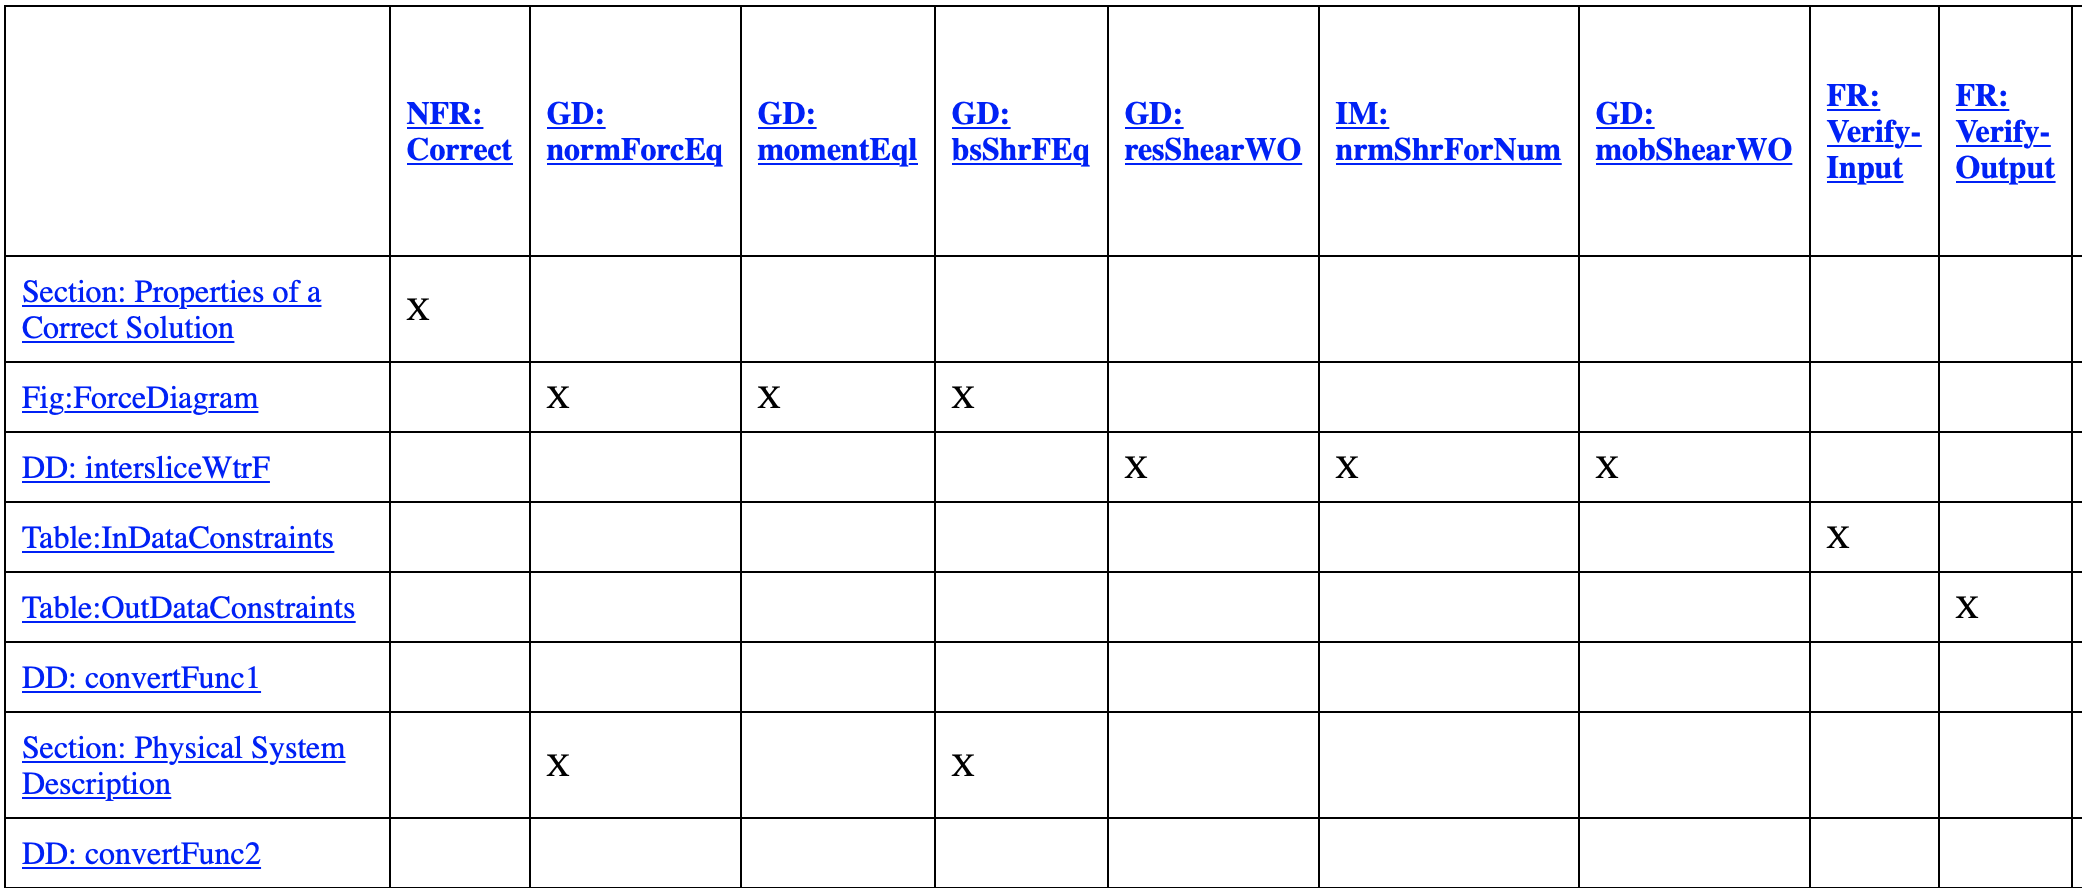
\includegraphics[width=\textwidth]{TraceBefore}
\caption{A portion of the automated traceability matrix for the Drasil example Slope Stability analysis Program (SSP).}\label{fig:traceBefore}
\end{figure}


%% Traceability matrix view design here
We mentioned a solution that introduces ``views" to a traceability matrix. Ideally we would like a constructor where we specify a list of chunk categories (i.e. assumptions, data definitions, etc.) where the list itself can be thought of as a one-dimensional view of a traceability matrix. The user facing syntax for such a constructor could be:

\begin{tcolorbox}
\begin{minted}{haskell}
TraceProg [{-Columns-} viewAssump]
  [{-Rows-} viewReqs, viewLikelyChgs]
\end{minted}
\end{tcolorbox}

When \haskell{TraceProg} is evaluated, \haskell{viewAssump}, \haskell{viewReqs}, and \haskell[breakanywhere, breakanywheresymbolpre=\textcolor{black}{-}]{viewLikelyChgs} are evaluated to retrieve traceability information that is then combined into a complete matrix. The constructor \haskell{TraceProg} addresses the issues described with the existing \haskell{TraceabilityProg} and \haskell{generateTraceTable} implementation thus eliminating the need for a user to perform specific incantations to create a traceability matrix. \haskell{TraceProg} enforces the content present in a traceability section is traceability related. Further, such a constructor inherently adds a sense of ordering and grouping to the displayed items within a matrix. Finally, such a generic \haskell{TraceProg} description allows for specification of many differing (even within the same document) matrices.

With a general guiding design of what we desire as a user-facing interface, we turn our attention to how \haskell{generateTraceTable} builds the traceability matrix. Most of the cross-referencing and chunk dependency tracking is performed by the following two functions: \haskell{generateTraceMap} and \haskell{generateRefbyMap}. These two functions produce tables that are added to \haskell{ChunkDB} and accessible through the \haskell{traceTable} and \haskell{refbyTable} fields, respectively. The information collected in these tables is accurate; we are adjusting the processes with which the information is displayed and organized from these tables in a more human-friendly manner.

%At the core of the single generated matrix is \haskell{traceMRow} and \haskell{traceMCol} which extract chunk \haskell{UID}s in a given dimension:

% \begin{tcolorbox}
% \begin{minted}{haskell}
% traceMRow :: ChunkDB -> [UID]
% traceMRow = nub . Map.keys . (^. refbyTable)
% 
% traceMCol :: ChunkDB -> [UID]
% traceMCol = nub . concat . Map.elems . (^. refbyTable)
% \end{minted}
% \end{tcolorbox}

%The keys of \haskell{refbyTable} are the \haskell{UID}s of chunks which are referred to, referees if you will. The values of \haskell{refbyTable} are the referrers to a given referee. With the current names (and subsequent uses) of \haskell{traceMRow} and \haskell{traceMCol}, we are transposing the idea of how we usually reason about tables: indepedent information along the top (and thus columns). Further the names of the functions do not provide enough meaningful context as someone or some cultures may prefer referrers to be along the top, we will rename \haskell{traceMRow} to \haskell{traceMReferees} and \haskell{traceMCol} to \haskell{traceMReferrers} to be more explicit and layout agnostic.

%With a list of \haskell{UID}s we have four methods to extract a reference from the lists and dependency information:

%\begin{tcolorbox}
%\begin{minted}{haskell}
%traceMHeader :: (ChunkDB -> [UID]) ->
%  SystemInformation -> [Sentence]
%traceMHeader f c = map (`helpToRefField` c) $ f $ _sysinfodb c
% 
%traceMRowHeader :: SystemInformation -> [Sentence]
%traceMRowHeader = traceMHeader traceMReferrers
%
%traceMColHeader :: SystemInformation -> [Sentence]
%traceMColHeader = traceMHeader traceMReferees
%
%traceMColumns :: ChunkDB -> [[UID]]
%traceMColumns c = map (`refbyLookup` (c ^. refbyTable)) $
%  traceMReferees c
%\end{minted}
%\end{tcolorbox}
%
%where \haskell{helpToRefField} is a function taking a \haskell{UID} and returns a \haskell{Ref} \haskell{Sentence} constructor. Finally, we examine how \haskell{generateTraceTable} uses these functions to create a traceability matrix:

%\begin{tcolorbox}
%\begin{minted}{haskell}
%generateTraceTable :: SystemInformation -> LabelledContent
%generateTraceTable c = llcc (makeTabRef "Tracey") $ Table
%  (EmptyS : (traceMColHeader c)) (makeTMatrix
%  	(traceMRowHeader c) (traceMColumns $ _sysinfodb c) $
%  	traceMReferrers $ _sysinfodb c)
%  (showingCxnBw traceyMatrix $ titleize' item +:+
%  	S "of Different" +:+ titleize' section_) True
%\end{minted}
%\end{tcolorbox}

%where \haskell{makeTMatrix} takes a list of row names, a list of all \haskell{UID}s referred to by each row, and a list of all \haskell{UID}s appearing in a column. The output of \haskell{makeTMatrix} is a row major two-dimensional list containing an ``X" in all cells where the row depends on a column. The \haskell{Table} constructor (a part of \textit{drasil-lang}'s \haskell{Content} data structure) takes a list of column headers followed by the row-major matrix contents, a label describing the table, and a boolean indicating whether to display the name of the table. Finally, the \haskell{makeTabRef} and \haskell{llcc} functions make the table referable --- using the \haskell{UID} ``Tracey" --- such that it conforms to the \haskell{TraceabiliyProg} constructor.

%We have mentioned our traceability matrix is transposed, based on the description of the arguments for \haskell{makeTMatrix}, the final argument is a list of columns, however in our case \haskell{traceMReferees} is the list of columns, whereas we're passing \haskell{traceMReferrers}. Further, the second argument ought to be row-major, however \haskell{traceMColumns} is column-major. Remedying these two issues results in:

%\begin{tcolorbox}
%\begin{minted}{haskell}
%traceMColumns :: ChunkDB -> [[UID]]
%traceMColumns c = map (flip traceLookup (c ^. traceTable)) $
%  traceMReferrers c
%
%generateTraceTable :: SystemInformation -> LabelledContent
%generateTraceTable c = llcc (makeTabRef "Tracey") $ Table
%  (EmptyS : (traceMColHeader c)) (makeTMatrix
%  	(traceMRowHeader c) (traceMColumns $ _sysinfodb c) $
%  	traceMReferees $ _sysinfodb c)
%  (showingCxnBw traceyMatrix $ titleize' item +:+
%  	S "of Different" +:+ titleize' section_) True
%\end{minted}
%\end{tcolorbox}

% which orients the traceability matrix as one would expect. We have decided to not change the name of \haskell{traceMColumns} as the name can be thought of as, ``for each row, the list of columns which ought to be marked."

%With the orientation of the traceability matrix addressed we can begin adding the appropriate infrastructure for views.
We begin by deciding on a type signature for the views. The inputs are a list of \haskell{UID}s of chunks, which may be a row or column (of traceability information) and a \haskell{ChunkDB}. The return type is a list of \haskell{UID}s to include in a given dimension of the traceability matrix. Further we add a type synonym, \haskell{TraceViewCat} (\textbf{Trace}ability \textbf{View} \textbf{Cat}egory), to present a more convenient idea of what the view functions perform.

%\begin{tcolorbox}
%\begin{minted}{haskell}
%type TraceViewCat = [UID] -> ChunkDB -> [UID]
%\end{minted}
%\end{tcolorbox}

The implementation for all \haskell{TraceViewCat} functions is to retrieve all chunks of a given type from a table in \haskell{ChunkDB}. The chunks retrieved match the ordering of the list passed to the \haskell{cdb} constructor, which will match the ordering of the chunks when displayed in the SRS, ensuring consistency in the displayed order, while allowing authors to control the ordering. \autoref{ci} simplified \haskell{ChunkDB} for \haskell{ConceptInstance}s by providing a single table for all of the chunks regardless of their domain; this design requires the ability to filter retrieved chunks. We wish to leverage the hierarchical structure of the \haskell{ConceptInstance} domains. Based on the domain being located, such as \haskell{reqDom}, we wish to include any domains within the \haskell{reqDom}ain, for example including both functional and non-functional requirements whose domains are both in the \haskell{reqDom}ain.

The two patterns of chunk lookups required for the traceability matrices are encoded in the functions: \haskell{traceView}, which retrieves and orders all chunks in a certain table, and \haskell{traceViewCC}, which specializes and extends \haskell{traceView} to lookup chunks in the \haskell{ConceptInstance} table and filter the results based on a desired domain. These two intermediary functions allow for specifying view categories in a trivial fashion:

\begin{tcolorbox}
\begin{minted}{haskell}
tvDataDefns :: TraceViewCat
tvDataDefns = traceView dataDefnTable

tvReqs :: TraceViewCat
tvReqs = traceViewCC reqDom
\end{minted}
\end{tcolorbox}

%\begin{tcolorbox}
%\begin{minted}{haskell}
%traceView :: HasUID a =>
%  Getting (UMap a) ChunkDB (UMap a) -> TraceViewCat
%traceView table _ = map (^. uid) . asOrderedList . (^. table)
%\end{minted}
%\end{tcolorbox}

%The \haskell{asOrderedList} function orders the chunks retrieved in the (unordered) table according to the order chunks were added in the \haskell{cdb} smart constructor, which also happens to be the way the \haskell{Assumptions} constructor orders chunks ensuring a consistent ordering throughout the document. We next create convenience \haskell{TraceViewCat} functions for different chunk types:

%\begin{tcolorbox}
%\begin{minted}{haskell}
%tvDataDefns :: TraceViewCat
%tvDataDefns = traceView dataDefnTable
%
%tvGenDefns :: TraceViewCat
%tvGenDefns = traceView gendefTable
%
%tvTheoryModels :: TraceViewCat
%tvTheoryModels = traceView theoryModelTable
%
%tvInsModels :: TraceViewCat
%tvInsModels = traceView insmodelTable
%\end{minted}
%\end{tcolorbox}
%
%enabling view categories for all chunks described in \textit{drasil-theory}. We encounter a mild complication, all \haskell{ConceptInstance}s are stored in a single table where we are required to distinguish which to view based on a domain. We enhance our original \haskell{traceView} and in the process rename it \haskell{traceViewFilt} adding an intermediary \haskell{traceView} providing the same interface to our views already created:

%\begin{tcolorbox}
%\begin{minted}{haskell}
%traceViewFilt :: HasUID a => (a -> Bool) ->
%  Getting (UMap a) ChunkDB (UMap a) -> TraceViewCat
%traceViewFilt f table _ = map (^. uid) . filter f .
%  asOrderedList . (^. table)
%
%traceView :: HasUID a =>
%  Getting (UMap a) ChunkDB (UMap a) -> TraceViewCat
%traceView = traceViewFilt (const True)
%\end{minted}
%\end{tcolorbox}
%
%We provide a similar intermediary function, named \haskell{traceViewCC}, to \haskell{traceView} for \haskell{ConceptInstance} domain lookup. \haskell{traceViewCC} makes use of the tree of domains created in \autoref{ci} where all sub-domains of a domain will be included in a view of a given domain. For example, specifying \haskell{chgProbDom} will include both likely change chunks (\haskell{likeChgDom}) and unlikely change chunks (\haskell{unlikeChgDom}). 

% Author Note: Simplifying code here to remove constraint and just be ConceptChunk
%\begin{tcolorbox}
%\begin{minted}{haskell}
%traceViewCC :: ConceptChunk -> TraceViewCat
%traceViewCC dom u c = traceViewFilt (isDomUnder (dom ^. uid) .
%  sDom . cdom) conceptinsTable u c
%  where
%    isDomUnder :: UID -> UID -> Bool
%    isDomUnder filtDom curr
%      | filtDom == curr = True
%      | not $ null $ getDom curr = isDomUnder filtDom
%        (sDom $ getDom curr)
%      | otherwise = False
%    getDom :: UID -> [UID]
%    getDom curr = cdom $ defLookup curr $ defTable c
%\end{minted}
%\end{tcolorbox}
%
%With \haskell{traceViewCC} we are able to implement views for \haskell{ConceptInstance} chunks in a simple manner similar to \textit{drasil-theory} chunks:

%\begin{tcolorbox}
%\begin{minted}{haskell}
%tvAssumps :: TraceViewCat
%tvAssumps = traceViewCC assumpDom
%tvGoals :: TraceViewCat
%tvGoals = traceViewCC goalStmtDom
%
%tvReqs :: TraceViewCat
%tvReqs = traceViewCC reqDom
%
%tvChanges :: TraceViewCat
%tvChanges = traceViewCC chgProbDom
%\end{minted}
%\end{tcolorbox}

Revisiting the desired interface, \haskell{TraceProg [{-Columns-}] [{-Rows-}]}, we are able to specify the view categories; however, we must provide means to flatten the list of \haskell{UID}s returned. While flattening the list is an easy task, the results must be filtered to ensure only chunks that appear in the SRS are included. While the design of \textit{drasil-docLang} currently seeds the SRS's content from the \haskell{ChunkDB}, this may not be the case in the future, or the chunks may be filtered in a description so only some chunks are included from the whole set of available chunks. With the current implementation of \haskell{TraceViewCat} functions, the traceability matrix may contain chunks that are part of the software system's description but not in the SRS. Thus we require a way to filter all of the returned chunks to those that appear in the SRS.

The \haskell{traceTable} field of \haskell{ChunkDB} captures the dependencies (values) of all chunks (keys) in an SRS. To generate \haskell{traceTable}, \textit{drasil-docLang} walks over a \haskell{DocDesc} collecting all chunks and their dependencies. If a chunk does not contain any dependencies it is still added to the table but with an empty value. We can leverage the keys of \haskell{traceTable} to ensure the chunks in the traceability matrices do appear in the SRS. We implement the required filtering alongside the flattening operation in \haskell{layoutUIDs}:

\begin{tcolorbox}
\begin{minted}{haskell}
layoutUIDs :: [TraceViewCat] -> ChunkDB -> [UID] -> [UID]
layoutUIDs a c e =
  filter (`elem` (Map.keys $ c ^. traceTable)) $
  concatMap (\x -> x e c) a
\end{minted}
\end{tcolorbox}

% where we filter the results based on the keys of \haskell{traceTable}, due to every chunk which appears in the SRS document having an entry in \haskell{traceTable} regardless of whether it is referenced by or refers to anything.\footnote{The same is not true for \haskell{refbyTable}.}
%By providing both the list of view categories as well as a \haskell{ChunkDB} we have a function which is from \haskell{[UID] -> [UID]} and convenient to \haskell{.} compose, for example, the definition of \haskell{traceMReferees} and \haskell{traceMReferrers} become:

%\begin{tcolorbox}
%\begin{minted}{haskell}
%traceMReferees :: ([UID] -> [UID]) -> ChunkDB -> [UID]
%traceMReferees f = f . nub . Map.keys . (^. refbyTable)
%
%traceMReferrers :: ([UID] -> [UID]) -> ChunkDB -> [UID]
%traceMReferrers f = f . nub . concat . Map.elems .
%  (^. refbyTable)
%\end{minted}
%\end{tcolorbox}
%
%A more complicated realization of view category filtering occurs with \haskell{traceMColumns}:
%
%\begin{tcolorbox}
%\begin{minted}{haskell}
%traceMColumns :: ([UID] -> [UID]) -> ([UID] -> [UID]) ->
%  ChunkDB -> [[UID]]
%traceMColumns fc fr c =
%  map ((\u -> filter (`elem` u) $ fc u) .
%  	flip traceLookup (c ^. traceTable)) $
%  traceMReferrers fr c
%\end{minted}
%\end{tcolorbox}
%
%where we perform an additional filter on the list of \haskell{UID}s returned to reduce ``selected" columns from all satisfying a particular list of views to those which are referred to by a given row.

%With the table construction supporting views --- omitting the adaptation of a few functions which only included changes to properly pass the partially applied \haskell{layoutUIDs} to the \haskell{traceM} functions discussed --- we introduce a new generation function, \haskell{generateTraceTableView}, to expose the new interface:

%\begin{tcolorbox}
%\begin{minted}{haskell}
%generateTraceTableView :: UID -> Sentence ->
%  [TraceViewCat] -> [TraceViewCat] ->
%  SystemInformation -> LabelledContent
%generateTraceTableView _ _ [] _ _ = error $ "..."
%generateTraceTableView u _ _ [] _ = error $ "..."
%generateTraceTableView u desc cols rows c =
%  llcc (makeTabRef u) $ Table
%    (EmptyS : ensureItems u (traceMColHeader colf c))
%    (makeTMatrix (ensureItems u $ traceMRowHeader rowf c)
%      (traceMColumns colf rowf cdb) $
%      traceMReferees colf cdb)
%  (showingCxnBw traceyMatrix desc) True where
%    cdb = _sysinfodb c
%    colf = layoutUIDs cols cdb
%    rowf = layoutUIDs rows cdb
%\end{minted}
%\end{tcolorbox}

%where \haskell{ensureItems} ensures a matrix dimension is not-empty. We continue to require a \haskell{Sentence} to describe what the traceability matrix is capturing. 

The final step is providing a function to specify a traceability matrix. A traceability matrix must include a \haskell{UID} (it can be referenced), a caption for the traceability matrix, the rows and columns of the matrix (\haskell{TraceViewCat}), and \haskell{SystemInformation} containing the \haskell{ChunkDB} needed for various table lookups. The function is named \haskell{generateTraceTableView} and produces a \haskell{LabelledContent} compatible for direct insertion into a \haskell{Document}. Care is taken within the function to ensure the number of views specified for rows and columns is not empty as a dimension of zero for a traceability matrix makes little sense.

The end goal of this chapter is to reduce the effort required for authors to encode systems in Drasil. One part of achieving the goal is to lift calls of \haskell{generateTraceTableView} into \textit{drasil-docLang} such that it is not exposed or used by authors directly. Instead, we encode the traceability information into \haskell{DocDesc} using a similar structure to \haskell{TraceProg} as outlined previously. An author is required to provide additional (human-oriented) context such as introduction text and a matrix's caption. We encode the \haskell{DocDesc} constructor as:
%The function \haskell{generateTraceTableView} requires a specify traceability matrices within \haskell{DocDesc}. A good start is the arguments passed to \haskell{generateTraceTableView}, ignoring the \haskell{SystemInformation} as that structure is available during processing of the \haskell{DocDesc}. We further require a \haskell{Sentence} outside of the arguments required for the new traceability matrix function to provide context within the introduction text to the traceability matrix section. With the list of parameters required to specify a traceability matrix, we create \haskell{TraceConfig}:

\begin{tcolorbox}
\begin{minted}{haskell}
data TraceConfig = TraceConfig UID [Sentence] Sentence
  [TraceViewCat] [TraceViewCat]
\end{minted}
\end{tcolorbox}

The second argument is the text describing what the traceability matrix shows. This text appears in the traceability section introduction. The third argument is the caption of the matrix; the fourth argument is the list of column views, and the final argument is the list of row views for the matrix. 

We extend the existing definition of \haskell{TraceabilitySec} to accommodate a list of \haskell{TraceConfig}s allowing for the specification of multiple traceability matrices, each providing a different view of chunk dependencies. Many of the bundled examples within Drasil (still) contain --- despite the single automated

\begin{figure}[H]
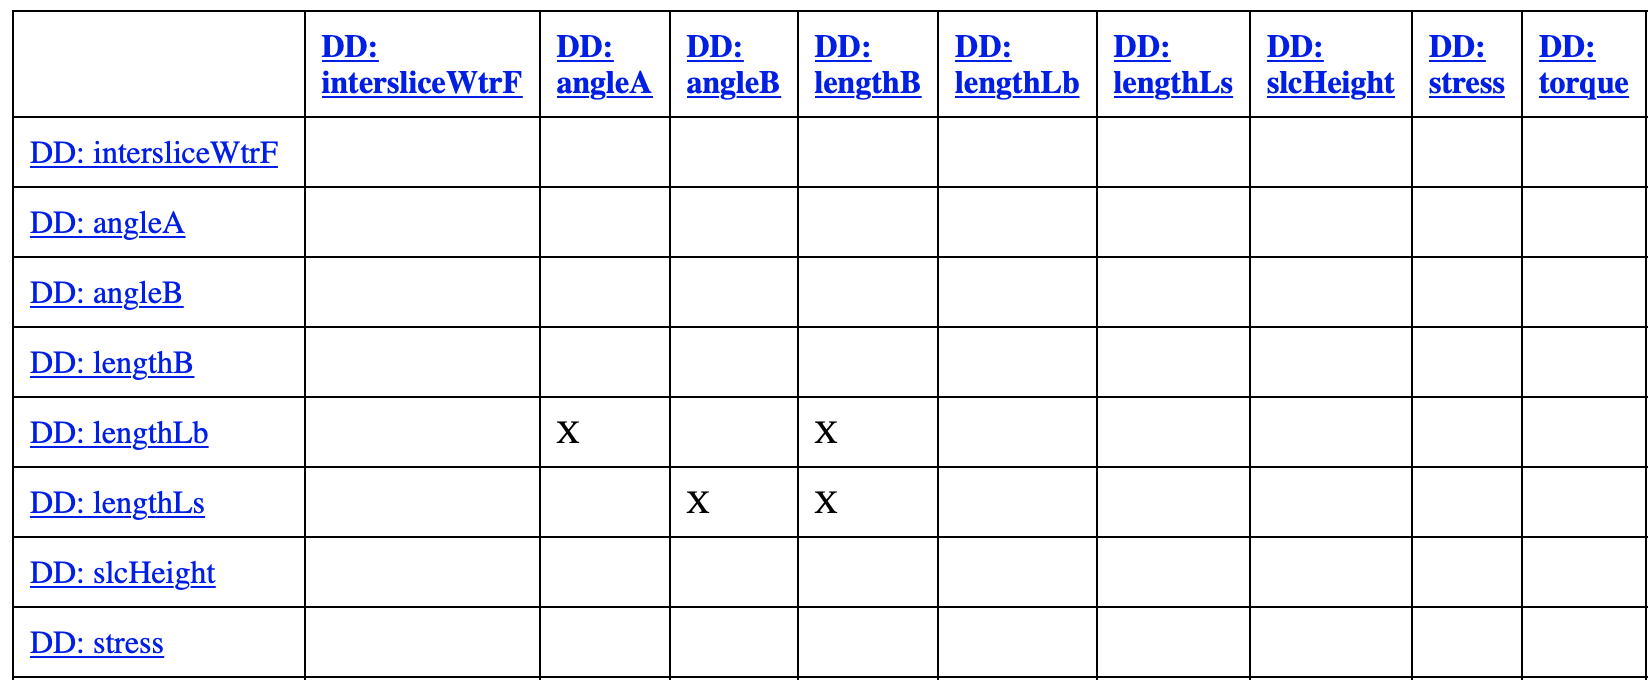
\includegraphics[width=\textwidth]{TraceAfter}
\caption{A portion of an automated traceability matrix constructed with \haskell{traceMatRefinement} in the Drasil example SSP.}\label{fig:traceAfter}
\end{figure}

\noindent matrix --- three traceability matrices maintained\footnote{Not really} manually. The new view functionality for traceability matrices allows the manual matrices to be replaced with automated variants. As the three configurations are common amongst all bundled examples, we encode a function describing each: \haskell[breakanywhere, breakanywheresymbolpre=\textcolor{black}{-}]{traceMatAssumpOther}, \haskell{traceMatRefinement}, and \haskell{traceMatOtherReq}. We encode a convenience function that packages all three together as \haskell{traceMatStandard}. \haskell{traceMatRefinement} replaces at least 50 lines (with the other standard matrices each removing approximately 50 lines each as well) in many bundled examples while producing more accurate output (\autoref{fig:traceAfter}) without requiring manual upkeep. The definition is:

% FIXME: Do items vs items here and as traceAfter since Assumptions aren't supposed to be here at this point....
\begin{tcolorbox}[breakable, toprule at break=0pt, bottomrule at break=0pt]
\begin{minted}{haskell}
traceMatRefinement :: TraceConfig
traceMatRefinement = TraceConfig "TraceMatRefvsRef"
  [plural Doc.dataDefn, plural Doc.thModel, plural
  Doc.genDefn, plural Doc.inModel +:+. S "with each other"]
  (titleize' item +:+ S "and Other" +:+ titleize' section_)
  [tvDataDefns, tvTheoryModels, tvGenDefns, tvInsModels]
  [tvDataDefns, tvTheoryModels, tvGenDefns, tvInsModels]
\end{minted}
\end{tcolorbox}

The implementation of a refined, higher-level \haskell{DocDesc} constructor for traceability matrices improves the display and flexibility of the matrices while moving \haskell{DocDesc} in the correct direction towards a declarative language. 
\clearpage

\section{Removing Boilerplate}\label{dlToDocLang}  % Pulling a fast one here. 

If we implement the desired declarative solution, one where \haskell{DocDesc} is hidden from authors and instead present a cleaner declarative \haskell{SRSDecl}, then we ought to investigate what functions exposed and used within \textit{drasil-example} take \haskell{DocDesc} as an argument. Any function that does will either need to be removed or altered to be used solely within \textit{drasil-docLang} as \haskell{DocDesc} will no longer be available in the sub-package. From \autoref{teExample} we have a set of incantations that take \haskell{DocDesc}, or a sub-structure of \haskell{DocDesc}, as an input:

% Author Note: Handwaving away the table of symbols constructors (ccss) that were lifted to docLang since there is some outstanding work that was out of scope on that.
\begin{tcolorbox}
\begin{minted}{haskell}
label :: TraceMap
label = generateTraceMap thisSRS

refBy :: RefbyMap
refBy = generateRefbyMap label

scs :: SCSSub
scs = getSCSSub thisSRS

dataDefn :: [DataDefinition]
dataDefn = getTraceMapFromDD scs

reqs :: [ReqChunk]
reqs = getTraceMapFromReqs scs

chgs :: [Change]
chgs = getTraceMapFromChgs scs
\end{minted}
\end{tcolorbox}

The desired model where information is contained within \haskell{ChunkDB} and retrieved to populate \haskell{DocDesc} renders \haskell{getSCSSub}, \haskell{getTraceMapFromDD}, \linebreak\haskell{getTraceMapFromReqs}, \haskell{getTraceMapFromChgs}, and others as unneeded. The functions previously served two purposes: gather chunks to populate a \haskell{ChunkDB} and gather chunks that are subsequently consumed for their \haskell{UID}s within \haskell{generateTraceMap}. The functions' use within individual examples is unnecessary and may be removed under the new model of chunk propagation.

The remaining SRS boilerplate within examples is \haskell{generateTraceMap} and \haskell{generateRefbyMap}. Both \haskell{generateTraceMap} and \haskell{generateRefbyMap} are computed from the SRS using \haskell{DocDesc} to populate a table, which are passed as arguments to the \haskell{cdb} constructor.

\haskell{generateTraceMap} is an excellent candidate to relocate to \textit{drasil-docLang}. It is a function that is required for automated traceability matrices to function. It does not provide any means of customization to a user calling it, as it simply extracts chunks from \haskell{DocDesc}. It is truly boilerplate, which users must remember to call. The reason for its existence within each example is because it becomes a table in \haskell{ChunkDB}, which is always constructed for a software system. We would instead like to delay construction of these tables to occur after a \haskell{ChunkDB} has been constructed and during \textit{drasil-docLang} processing of \haskell{DocDesc}. \haskell{generateRefbyMap} transitively depends on the \haskell{DocDesc}, as it inverts the map produced by \haskell{generateTraceMap}, allowing both to be moved together, while \haskell{generateRefbyMap} can be an afterthought to a design for \haskell{generateTraceMap}.

All tables within \haskell{ChunkDB} implement Lenses~\cite{Lenses} allowing for modification after initial construction. If we leverage this existing feature, we can move traceability information generation (and subsequent table updates within \haskell{ChunkDB}) to immediately after \haskell{DocDesc} is constructed. Due to the new information propagation flow this chapter is enacting, traceability information should not be completely available until \haskell{DocDesc} is constructed and refers specifically to the SRS document. If we were to modify which chunks appeared in an SRS (through possible elaboration when constructing \haskell{DocDesc} from \haskell{SRSDecl}) we would like the traceability information to include the most recent data as opposed to ``stale" data from an earlier point in the artefact generation process. Another benefit of delaying traceability information extraction is we remove the need for users to be concerned about how traceability information is gathered and stored and can simplify the \haskell{cdb} constructor to remove the two tables that are later populated.

In an effort to realize the relocation of \haskell{generateTraceMap} and \linebreak\haskell{generateRefbyMap}, we should examine the definition of the candidate destination function, \haskell{mkDoc}, a function that transforms a \haskell{DocDesc} --- when we are done elaborating an \haskell{SRSDecl} --- to a \textit{drasil-lang} \haskell{Document}, ideally behaving as the \textit{drasil-docLang} transformation function. \haskell{mkDoc}'s input is the finalized \haskell{DocDesc} making it an appropriate location to derive traceability information and amend the \haskell{ChunkDB} prior to construction of the traceability matrices. We construct a function, \haskell{fillTraceMaps}, which \haskell{set}s the two traceability related tables after invoking \haskell{generateTraceMap} and \haskell{generateRefbyMap}, and call the function early within \haskell{mkDoc} before any \haskell{DocDesc} constructors are translated to \haskell{Document} constructors.

%\begin{tcolorbox}
%\begin{minted}{haskell}
%mkDoc :: DocDesc -> (IdeaDict -> IdeaDict -> Sentence) ->
%  SystemInformation -> Document
%mkDoc l comb si@SI {_sys = sys, _kind = kind,
%  _authors = authors} = Document
%	(nw kind `comb` nw sys) (foldlList Comma List $
%	  map (S . name) authors) (mkSections si l)
%\end{minted}
%\end{tcolorbox}

%where \haskell{mkSections} translates each \haskell{DocDesc} constructor into a \textit{drasil-lang} \haskell{Section}. At the point where \haskell{mkSections} is called, we have the final \haskell{DocDesc}. If we are to update the \haskell{_sysinfodb} within \haskell{SystemInformation} to contain traceability information, it would include the final state of \haskell{DocDesc}. To perform the action of populating the traceability information named \haskell{fillTraceMaps}, updating \haskell{SystemInformation} according to a \haskell{DocDesc}:

%\begin{tcolorbox}
%\begin{minted}{haskell}
%fillTraceMaps :: DocDesc ->
%  SystemInformation -> SystemInformation
%fillTraceMaps dd si@SI{_sysinfodb = db} = si {_sysinfodb =
%  set refbyTable (generateRefbyMap tdb) $
%  set traceTable tdb db} where
%    tdb = generateTraceMap dd
%\end{minted}
%\end{tcolorbox}
%
%where \haskell{set} is a Lens function to modify the table within the \haskell{ChunkDB} \haskell{db}. Updating \haskell{mkDoc} to populate the traceability tables yields:
%
%\begin{tcolorbox}
%\begin{minted}{haskell}
%mkDoc :: DocDesc -> (IdeaDict -> IdeaDict -> Sentence) ->
%  SystemInformation -> Document
%mkDoc l comb si@SI {_sys = sys, _kind = kind,
%  _authors = authors} = Document
%	(nw kind `comb` nw sys) (foldlList Comma List $
%	  map (S . name) authors)
%	(mkSections (fillTraceMaps l si) l)
%\end{minted}
%\end{tcolorbox}

The last function, although not taking \haskell{DocDesc} as input, is an incantation from \autoref{teExample} requiring migration or removal. The function, \haskell{collectUnits}, requires a list of symbols to determine which units are involved in an SRS and a \haskell{ChunkDB}. It is not mandatory to migrate to \textit{drasil-docLang}; however, the action performed is specifically for a \haskell{DocDesc} section. With the introduction of \haskell{SRSDecl}, this should not be something an author is manually required to perform. \haskell{collectUnits} extracts units from the provided symbols, which are used to display a table of units within the SRS. Similar to the traceability matrix, \haskell{collectUnits}' action is specifically for a section. Failure for a user to perform an action should not result in an inaccurate or empty table of units section, as such, \haskell{collectUnits} should be invoked by \textit{drasil-docLang} as needed to ensure consistency throughout the document and effectively be ``magic" for the system implementor. 

To migrate \haskell{collectUnits} to \textit{drasil-docLang}, we require means to extract the used symbols as opposed to having them explicitly passed by the user. Symbols within \haskell{DocDesc} are contained within \haskell{Sentence}s and \haskell{Expr}essions. Conveniently, two functions exist to scan \haskell{DocDesc} and extract such elements: \haskell{getDocDesc} and \haskell{egetDocDesc}, respectively. Another function (\haskell{ccss'}) exists that extract symbols, contained in \haskell{QuantityDict}, from \haskell{Sentence} and \haskell{Expr}. Combining these components together we have, \haskell[breakanywhere, breakanywheresymbolpre=\textcolor{black}{-}]{extractUnits}, a function that extracts units given a \haskell{DocDesc}:

\begin{tcolorbox}
\begin{minted}{haskell}
extractUnits :: DocDesc -> ChunkDB -> [UnitDefn]
extractUnits dd cdb = collectUnits cdb $
  ccss' (getDocDesc dd) (egetDocDesc dd) cdb
\end{minted}
\end{tcolorbox}

\haskell{extractUnits} allows for the \haskell{collectUnits} boilerplate to be removed from each example. The function is invoked during the expansion of \haskell{DocDesc}'s constructor to produce a table of units. Deferral of unit collection allows it to occur in the function that generates the table of units reducing the surface of functions that know \textit{how} the table of units is generated and concentrate the knowledge in the area of interest.

%\haskell{extractUnits} provides an advantage over the previous user-specified method: it only includes units from symbols which appear in the final SRS. The previous method allowed for an over-specification of symbols leading to entries in the table of units of units which did not appear within the final document. The last step to remove the user-required boilerplate is to use \haskell{extractUnits} when a \haskell{DocDesc} \haskell{TUnit} or \haskell{TUnit'} constructor is specified:

%\begin{tcolorbox}
%\begin{minted}{haskell}
%mkSubRef :: SystemInformation -> RefTab -> Section
%mkSubRef si' TUnits = mkSubRef si' $ TUnits' defaultTUI
%mkSubRef SI {_sysinfodb = db} (TUnits' con) =
%  tableOfUnits (nub $ sortBy compUnitDefn $
%  	extractUnits dd db) (tuIntro con)
%\end{minted}
%\end{tcolorbox}
%
%where \haskell{mkSubRef} populates reference tables when constructing the reference section of the Smith et al. SRS template\cite{smith2005new}, \haskell{compUnitDefn} provides lexicographic-like ordering to units, and \haskell{dd} is a \haskell{DocDesc} from an outer-scope function omitted in the code snippet displayed.

The migration of \haskell{collectUnits} has removed all incantations required for proper SRS function shown in \autoref{teExample} through relocation of many functions to \textit{drasil-docLang}, moving the goal of \haskell{SRSDecl} closer to reality.


\section{More Boilerplate?}\label{dlMultiplate}

In \autoref{diFraming} we made \haskell{DocDesc}'s \haskell{Assumptions} constructor consistent with the other chunk constructors, as \haskell{DocDesc} will soon be hidden within \textit{drasil-docLang}. We ought to address the introspection passes we used in \autoref{dlToDocLang} --- namely \haskell{generateTraceMap}, \haskell{getDocDesc}, and \haskell{egetDocDesc} --- to ensure their inclusion of content present in \haskell{Assumptions}, something that has not been done due to the anomalous constructor.

Repeatedly in this chapter we have discussed the traceability matrix and the enhancements provided, however, the \haskell{Assumptions} constructor has complicated efforts to include \haskell{ConceptInstance}s related to assumptions within the traceability matrix. \haskell{generateTraceMap} extracts traceability information from the SRS, we will use it as a starting point to investigate including assumptions in the matrices. Examining the function shows:

\begin{tcolorbox}
\begin{minted}{haskell}
generateTraceMap :: DocDesc -> TraceMap
generateTraceMap a = Map.unionsWith (\(w,x) (y,z) -> (w ++ y,
  ordering x z)) [traceMap' extractSFromNotes tt,
  traceMap' extractSFromNotes gd,
  traceMap' extractSFromNotes ddef,
  traceMap' extractSFromNotes imod,
  traceMap' extractSFromDeriv gd,
  traceMap' extractSFromDeriv ddef,
  traceMap' extractSFromDeriv imod,
  ...]
  where
    tt   = getTraceMapFromTM $ getSCSSub a
    gd   = getTraceMapFromGD $ getSCSSub a
    imod = getTraceMapFromIM $ getSCSSub a
    ddef = getTraceMapFromDD $ getSCSSub a
    ...
    ordering x y = if x == y then x else error "..."
\end{minted}
\end{tcolorbox}

%where \haskell{extractSFrom} functions extract \haskell{Sentence}s from chunks (following typeclass constraints) and \haskell{traceMap'} extracts references from \haskell{Sentence}s. 

Examining \haskell{getTraceMapFrom} functions reveals:

\begin{tcolorbox}[breakable, toprule at break=0pt, bottomrule at break=0pt]
\begin{minted}{haskell}
getTraceMapFromTM :: [SCSSub] -> [TheoryModel]
getTraceMapFromTM (TMs _ _ t:_) = t
getTraceMapFromTM (_:tl)        = getTraceMapFromTM tl
getTraceMapFromTM []            = error "No TM found."

getTraceMapFromGD :: [SCSSub] -> [GenDefn]
getTraceMapFromGD (GDs _ _ gd _:_) = gd
getTraceMapFromGD (_:tl)           = getTraceMapFromGD tl
getTraceMapFromGD []               = []
\end{minted}
\end{tcolorbox}

Although only two of the functions have been reproduced, all the \haskell[breakanywhere, breakanywheresymbolpre=\textcolor{black}{-}]{getTraceMapFrom} functions follow a similar template. Between the two functions shown, their empty behaviour differs for unexplained reasons. Each function's ``useful" results come from the first pattern match, the other two pattern matches can be seen as structural noise. 

Before continuing with the original idea to include \haskell{Assumptions} in introspective \haskell{DocDesc} passes, we should survey the other two passes to discern whether boilerplate is just as pervasive.

Beginning with \haskell{getDocDesc} we have:

\begin{tcolorbox}
\begin{minted}{haskell}
getDocDesc :: DocDesc -> [Sentence]
getDocDesc = concatMap getDocSec

getDocSec :: DocSection -> [Sentence]
getDocSec (RefSec r)           = getRefSec r
getDocSec (IntroSec i)         = getIntrosec i
getDocSec (StkhldrSec s)       = getStk s
getDocSec (GSDSec g)           = getGSD g
getDocSec (SSDSec s)           = getSSD s
...

getSSD :: SSDSec -> [Sentence]
getSSD (SSDProg ssd) = concatMap getSSDSub ssd

getSSDSub :: SSDSub -> [Sentence]
getSSDSub (SSDProblem pd)    = getProblem pd
getSSDSub (SSDSolChSpec sss) = getSol sss

getProblem :: ProblemDescription -> [Sentence]
getProblem (PDProg s x _) = s : concatMap getSec x

getSol :: SolChSpec -> [Sentence]
getSol (SCSProg x) = concatMap getSCSSub x
...
\end{minted}
\end{tcolorbox}

Observation of the functions shown indicates \haskell{getDocDesc} is simply a fold over \haskell{DocDesc}. Some functions such as \haskell{getSSD} are a simple \haskell{concatMap}! In all the code displayed, comprising a part of \haskell{getDocDesc}, only one line actually extracts a \haskell{Sentence}! The (portion of a) line is the second pattern match of \haskell{getProblem}. The rest is dealing exclusively with traversing the structure. Does \haskell{egetDocDesc} improve on the situation?

\begin{tcolorbox}[breakable, toprule at break=0pt, bottomrule at break=0pt]
\begin{minted}{haskell}
egetSSD :: SSDSec -> [Expr]
egetSSD (SSDProg ssd) = concatMap egetSSDSub ssd

egetSSDSub :: SSDSub -> [Expr]
egetSSDSub (SSDProblem p)   = egetProblem p
egetSSDSub (SSDSolChSpec s) = egetSol s

egetProblem :: ProblemDescription -> [Expr]
egetProblem (PDProg _ s _) = concatMap egetSec s

egetSol :: SolChSpec -> [Expr]
egetSol (SCSProg s) = concatMap egetSCSSub s
\end{minted}
\end{tcolorbox}

A sample of functions called through \haskell{egetDocDesc} demonstrates a similar situation albeit worse. Not only do none of the functions returning \haskell{[Expr]} produce anything of value and only traverse the structure, they omit traversing \haskell{Sentence}s and thus \textbf{miss} all \haskell{Expr}s embedded in \haskell{Sentence}s! \haskell{Sentence}s include a constructor (\haskell{E}) used to embed \haskell{Expr}. This can be observed in the code comprising \haskell{getProblem} and \haskell{egetProblem}, the \haskell{Sentence} extracted in the former is ignored in the latter.

With no framework in place for \haskell{DocDesc} to provide convenient means to add an introspective pass, we impair the desired behaviour for \haskell{DocDesc} to be a structure designed to be interrogated. If it remains as tedious and boilerplate-heavy to introduce a pass, it is entirely possible other developers and maintainers in a rush may ``hack together" a partial (in the functional sense) solution that easily breaks. Further, each introduced pass will inhibit \haskell{DocDesc}'s ability to change and evolve. Developer's desire to alter \haskell{DocDesc} will also be stifled due to the sheer amount of boilerplate requiring modification.

A desirable solution is one that abstracts the boilerplate away, yet allows ``random access" into the substructures that make up \haskell{DocDesc}. Another useful feature would be a mechanism to fold \haskell{DocDesc} as current passes all return a list of \textit{something}. A design with both features would allow for a streamlined re-implementation of the three existing passes and reduce the effort and time to write additional passes. 

% Literally a hack to support a type signature not bound to a function
The solution exists within the Haskell ecosystem as the package Multiplate~\cite{multiplate}. Multiplate provides a typeclass, \haskell{Multiplate}, that when implemented on structure provides the two features (random access, folding) desired. The data structure implementing \haskell{Multiplate} is a record where each field becomes a point of random access. Without delving too far into the details of multiplate, the structure includes a type variable \haskell{f} where each field is a function from \haskell{a ->} \haskell{f} \haskell{a}, relying on applicative functors to aid in the removal of the boilerplate.

Delving straight into Drasil's use of multiplate, we create a data structure \haskell{DLPlate} including a field for each sub-structure of \haskell{DocDesc} exposing the widest surface for random access.

\begin{tcolorbox}[breakable, toprule at break=0pt, bottomrule at break=0pt]
\begin{minted}{haskell}
data DLPlate f = DLPlate {
    docSec :: DocSection -> f DocSection,
    ...
    ssdSec :: SSDSec -> f SSDSec,
    ssdSub :: SSDSub -> f SSDSub,
    pdSec :: ProblemDescription -> f ProblemDescription,
    pdSub :: PDSub -> f PDSub,
    scsSub :: SCSSub -> f SCSSub,
    ...
  }
\end{minted}
\end{tcolorbox}

The \haskell{Multiplate} typeclass requires definitions for two functions \haskell[breakanywhere, breakanywheresymbolpre=\textcolor{black}{-}]{multiplate} and \haskell{mkPlate}. \haskell{multiplate} describes how each data structure relates to each field within the plate. We realize this for \haskell{DLPlate} as:

\begin{tcolorbox}[breakable, toprule at break=0pt, bottomrule at break=0pt]
\begin{minted}{haskell}
instance Multiplate DLPlate where
  multiplate p = DLPlate ds res intro intro' stk stk' gs gs'
    ss ss' pd pd' sc rs rs' lcp ucp ts es acs aps where
    ...
    ds (SSDSec x) = SSDSec <$> ssdSec p x
    ...

    res (RefProg c x) = RefProg <$> pure c <*> pure x
    ...
    ss (SSDProg prog) = SSDProg <$> traverse (ssdSub p) prog
    ss' (SSDProblem prog) = SSDProblem <$> pdSec p prog
    ss' (SSDSolChSpec (SCSProg spec)) = SSDSolChSpec .
      SCSProg <$> traverse (scsSub p) spec
    pd (PDProg s sect progs) = PDProg <$> pure s <*>
      pure sect <*> traverse (pdSub p) progs
    pd' (TermsAndDefs s cs) = TermsAndDefs <$> pure s <*>
      pure cs
    pd' (Goals s ci) = Goals <$> pure s <*> pure ci
    pd' (PhySysDesc nm s lc c) = PhySysDesc <$> pure nm <*>
      pure s <*> pure lc <*> pure c
    sc (Assumptions c) = Assumptions <$> pure c
    sc (TMs s f t) = TMs <$> pure s <*> pure f <*> pure t
    sc (GDs s f g d) = GDs <$> pure s <*> pure f <*>
      pure g <*> pure d
    sc (DDs s f dd d) = DDs <$> pure s <*> pure f <*>
      pure dd <*> pure d
    sc (IMs s f i d) = IMs <$> pure s <*> pure f <*>
      pure i <*> pure d
    sc (Constraints s c) = Constraints <$> pure s <*> pure c
    sc (CorrSolnPpties c cs) = CorrSolnPpties <$> pure c <*>
      pure cs
    ...
\end{minted}
\end{tcolorbox}

Many of the functions alluded to in the first line have been elided for brevity.

The second function required for \haskell{Multiplate} is \haskell{mkPlate}, which takes a function used to construct each field of the completely instantiated plate. For \haskell{DLPlate} this function is implemented as:

\begin{tcolorbox}
\begin{minted}{haskell}
instance Multiplate DLPlate where
  mkPlate b = DLPlate (b docSec) (b refSec) (b introSec)
    (b introSub) (b stkSec) (b stkSub) (b gsdSec) (b gsdSub)
    (b ssdSec) (b ssdSub) (b pdSec) (b pdSub) (b scsSub)
    (b reqSec) (b reqSub) (b lcsSec) (b ucsSec) (b traceSec)
    (b offShelfSec) (b auxConsSec) (b appendSec)
\end{minted}
\end{tcolorbox}

We have completed all the boilerplate required to produce introspection passes for \haskell{DocDesc}!

We begin the task of migrating the existing passes to \haskell{DLPlate}. In the instantiated plates, we make heavy use of the Glasgow Haskell Compiler Haskell language extension \texttt{LambdaCase}\footnote{\url{https://downloads.haskell.org/~ghc/latest/docs/html/users_guide/glasgow_exts.html\#lambda-case}}. \texttt{LambdaCase} introduces syntax sugar allowing replacement of

\begin{tcolorbox}
\begin{minted}{haskell}
\a -> case a of
  p1 -> ...
  p2 -> ...

-- With
\case 
  p1 -> ...
  p2 -> ...
\end{minted}
\end{tcolorbox}

Multiplate provides the function \haskell{foldFor} to fold a plate instantiation into a \haskell{Monoid}. Due to the folding operation performed on the plate, the functor used to realize the type transformation is \haskell{Constant}, defined as\footnote{\url{http://hackage.haskell.org/package/transformers-0.5.6.2/docs/src/Data.Functor.Constant.html\#Constant}}:

\begin{tcolorbox}
\begin{minted}{haskell}
newtype Constant a b = Constant {getConstant :: a}
\end{minted}
\end{tcolorbox}

We begin by implementing a \haskell{DLPlate} to extract ``things" from \haskell{Section}s and \haskell{Content}s within \textit{drasil-lang}'s \haskell{Document} --- as \haskell{DocDesc} contains many constructors including \haskell{Content}s --- which may contain \haskell{Sentence} or \haskell{Expr}. We describe the function with as generic a type as possible, being able to fold \clearpage to any monoid and allowing the caller to specify functions to describe \textit{what} is taken from the two \haskell{Document} types when encountered:

\begin{tcolorbox}
\begin{minted}{haskell}
secConPlate :: Monoid b => (forall a. HasContents a =>
  [a] -> b) -> ([Section] -> b) -> DLPlate (Constant b)
\end{minted}
\end{tcolorbox}

\haskell{(forall a. HasContents a => [a] -> b)} is a second rank type, as the passed function should handle any structure implementing the \haskell{HasContents} typeclass. Glassgow Haskell Compiler requires specifying the \texttt{Rank2Types}\footnote{\url{https://downloads.haskell.org/~ghc/latest/docs/html/users_guide/glasgow_exts.html\#extension-Rank2Types}} language extension for the specified type signature to typecheck. 

Next is to produce a plate observing the sub-structures of interest. The multiplate library includes a function \haskell{purePlate} providing a \haskell{pure} default for each field we do not implement. Further, we would like the \haskell{DocDesc} to be exhaustively folded, requiring either multiplate's \haskell{preorderFold} or \haskell[breakanywhere, breakanywheresymbolpre=\textcolor{black}{-}]{postorderFold}. For the plates being written, the order does not matter, and as such \haskell{preorderFold} has been arbitrarily chosen. Having described the functions required to produce a plate instantiation, we realize \haskell{secConPlate} as:

\begin{tcolorbox}[breakable, toprule at break=0pt, bottomrule at break=0pt]
\begin{minted}{haskell}
secConPlate mCon mSec = preorderFold $ purePlate {
  ...
  gsdSec = Constant <$> \case
    (GSDProg s1 c1 c2 s2) -> mconcat [mSec s1, mCon [c1],
      mCon c2, mSec s2]
    (GSDProg2 _) -> mempty,
  ...
  pdSec = Constant <$> \(PDProg _ s _) -> mSec s,
  pdSub = Constant <$> \case
    (TermsAndDefs _ _) -> mempty
    (PhySysDesc _ _ lc c) -> mCon [lc] `mappend` mCon c
    (Goals _ _) -> mempty,
  ...
}
\end{minted}
\end{tcolorbox}

Many fields have been omitted for brevity. 

With a plate to extract \haskell{Content}s and \haskell{Section}s, we may now describe a plate to extract \haskell{Sentence}s. In a similar manner we keep \haskell{sentencePlate} as abstract by defining it over all \haskell{Monoid}s and including a function to translate \haskell{Sentence} to another type for embedding the plate within another plate. We describe the plate as:
\clearpage
\begin{tcolorbox}
\begin{minted}{haskell}
sentencePlate :: Monoid a =>
  ([Sentence] -> a) -> DLPlate (Constant a)
sentencePlate f = appendPlate
  (secConPlate (f . concatMap getCon') $
    f . concatMap getSec) $
  preorderFold $ purePlate {
    ...
    stkSec = Constant . f <$> \case
      (StkhldrProg _ s) -> [s]
      _ -> [],
    stkSub = Constant . f <$> \case
      (Client _ s) -> [s]
      (Cstmr _) -> [],
    pdSec = Constant . f <$> \(PDProg s _ _) -> [s],
    ...
    scsSub = Constant . f <$> \case
      (Assumptions c) -> map (^. defn) c
      ...
\end{minted}
\end{tcolorbox}

We include \haskell{secConPlate} with \haskell{sentencePlate} as \haskell{Document} constructs embed \haskell{Sentence}s. \haskell{getCon'} and \haskell{getSec} are functions to extract \haskell{Sentence}s from the \haskell{Document} constructs. Similar to the previous plate, we have omitted many fields for brevity. Of interest is the \haskell{pdSec} field that provides the same functionality as \haskell{getProblem} from the previous implementation, but without the boilerplate. Further, we have included \haskell{Assumption} in the new plate beginning to address the original purpose for examining the introspective passes. The final step is using the \haskell{sentencePlate} in \haskell{getDocDesc}:

\begin{tcolorbox}
\begin{minted}{haskell}
fmGetDocDesc :: DLPlate (Constant [a]) -> DocDesc -> [a]
fmGetDocDesc p = concatMap (foldFor docSec p)

getDocDesc :: DocDesc -> [Sentence]
getDocDesc = fmGetDocDesc (sentencePlate id)
\end{minted}
\end{tcolorbox}

\haskell{foldFor} folds \haskell{DLPlate} starting with the \haskell{docSec} field (the top-level structure) and strips the \haskell{Constant} functor off the result.

We repeat the same process as \haskell{sentencePlate} for \haskell{Expr}:

\begin{tcolorbox}[breakable, toprule at break=0pt, bottomrule at break=0pt]
\begin{minted}{haskell}
exprPlate :: DLPlate (Constant [Expr])
exprPlate = sentencePlate (concatMap sentToExp) `appendPlate`
  secConPlate (concatMap egetCon')
  (concatMap egetSec) `appendPlate`
  (preorderFold $ purePlate {
    scsSub = Constant <$> \case
      (TMs _ _ t) -> let r = concatMap (
                             \x -> x ^. invariants ++
                                defExp (x ^. defined_quant ++
                                x ^. defined_fun) ++
                             r (x ^. valid_context)) in r t
      (DDs _ _ d _) -> map sy d ++ defExp d
      (GDs _ _ g _) -> expRel g
      (IMs _ _ i _) -> expRel i
      _ -> [],
    auxConsSec = Constant <$>
      \(AuxConsProg _ qdef) -> defExp qdef
  })where
    defExp :: DefiningExpr a => [a] -> [Expr]
    defExp = map (^. defnExpr)
    expRel :: ExprRelat a => [a] -> [Expr]
    expRel = map (^. relat)
\end{minted}
\end{tcolorbox}

\haskell{sentToExp} extracts any \haskell{Expr}s from \haskell{Sentence}s. \haskell{exprPlate} is only 10 lines longer (and displayed in full) than the snippet showing the previous \haskell{Expr} introspection pass, which contained only boilerplate. \haskell{exprPlate} also remedies the the previous method missing extraction of expressions from \haskell{Sentence}s. Any \haskell{Sentence} extracted by \haskell{sentencePlate} has any \haskell{Expr}s extracted without knowing where the sentences are! 

Similar to \haskell{getDocDesc}, \haskell{egetDocDesc} becomes:

\begin{tcolorbox}
\begin{minted}{haskell}
egetDocDesc :: DocDesc -> [Expr]
egetDocDesc = fmGetDocDesc exprPlate
\end{minted}
\end{tcolorbox}

Finally, we are back to where we started, adding \haskell{Assumptions} to the traceability information. We combine this addition with an introspection pass extracting what each chunk traces to:

\begin{tcolorbox}[breakable, toprule at break=0pt, bottomrule at break=0pt]
\begin{minted}{haskell}
dependencyPlate :: DLPlate (Constant [(UID, [UID])])
dependencyPlate = preorderFold $ purePlate {
  ...
  scsSub = Constant <$> \case
    (Assumptions a) -> getDependenciesOf [defs] a
    ...
    (DDs _ _ d _) -> getDependenciesOf ... d
    (GDs _ _ g _) -> getDependenciesOf ... g
    (IMs _ _ i _) -> getDependenciesOf ... i
    _ -> [],
  ...
} where
  getDependenciesOf :: HasUID a => [a -> [Sentence]] ->
    [a] -> [(UID, [UID])]
  getDependenciesOf fs = map (\x -> (x ^. uid,
    concatMap (lnames' . ($ x)) fs))
  defs :: Definition a => a -> [Sentence]
  defs x = [x ^. defn]
  ...

generateTraceMap :: [DocSection] -> TraceMap
generateTraceMap = traceMap .
  concatMap (foldFor docSec dependencyPlate)
\end{minted}
\end{tcolorbox}

\haskell{lnames'} extracts references from \haskell{Sentence}s. While some chunks have been elided for brevity, it is clear this is much cleaner than the previous implementation. Further, adding dependencies of \haskell{Assumptions} required only a single line of code heavily reducing the effort to add additional constructors and chunks to the traceability matrix.

What began as a simple task to add \haskell{Assumptions} to traceability matrices quickly revealed the complexity and tedium required to interrogate \haskell{DocDesc}. The effort required did not align with the desired model of document processing we have in mind for \textit{drasil-docLang}. To remedy the issue, we leveraged multiplate to abstract away the boilerplate and provide clean, random-access introspection to \haskell{DocDesc}.

\section{\haskell{SRSDecl}}\label{dlSRSDecl}
With \haskell{dependencyPlate} implemented, we have achieved what we set out to perform and completed all the refactoring work necessary for \haskell{DocDesc} to be information complete while giving way to \haskell{SRSDecl} to be the declarative exposed language of SRS documents.

Due to \haskell{SRSDecl} and \haskell{DocDesc} being closely related at the moment, we leverage \haskell{DocDesc} when implementing \haskell{SRSDecl} to ease the expansion process. This allows both data structures to share many sub-structures (which do not differ) making the transformation only that of using the appropriate constructor. 

We provide the outer most data structure of \haskell{SRSDecl} to demonstrate the level of overlap with the \haskell{DL} prefix indicating the data structure is that of \haskell{DocDesc}:

\begin{tcolorbox}
\begin{minted}{haskell}
type SRSDecl = [DocSection]

data DocSection = RefSec DL.RefSec
                | IntroSec DL.IntroSec
                | StkhldrSec DL.StkhldrSec
                | GSDSec DL.GSDSec
                | SSDSec SSDSec
                | ReqrmntSec ReqrmntSec
                | LCsSec
                | UCsSec
                | TraceabilitySec DL.TraceabilitySec
                | AuxConstntSec DL.AuxConstntSec
                | Bibliography
                | AppndxSec DL.AppndxSec
                | OffShelfSolnsSec DL.OffShelfSolnsSec
\end{minted}
\end{tcolorbox}

For brevity we examine the \haskell{SRSDecl} \haskell{SCSSub} (a substructure of \haskell{SSDSec}) that exhibits all behavioural features of \haskell{SRSDecl}'s transformation we wish to show:

% Author Note: Un-GADTed
\begin{tcolorbox}
\begin{minted}{haskell}
data SCSSub = Assumptions
  | TMs [Sentence] Fields
  | GDs [Sentence] Fields DL.DerivationDisplay
  | DDs [Sentence] Fields DL.DerivationDisplay
  | IMs [Sentence] Fields DL.DerivationDisplay
  | Constraints Sentence [UncertainChunk]
  | CorrSolnPpties [ConstrainedChunk] [Contents]
\end{minted}
\end{tcolorbox}

The \haskell{Constraints} and \haskell{CorrSolnPpties} constructors continue to contain an explicit list of chunks as the chunks specified are not stored with full information within \haskell{ChunkDB}. The only required expansion operation, for the other constructors in \haskell{SCSSub}, is to look up chunks in a table of \haskell{ChunkDB} and provide the ordered list of chunks as an argument to the \haskell{DocDesc} constructor. The chunks implemented as \haskell{ConceptInstance} contain a second step similar to \autoref{dlTraceMat} requiring domain filtering to obtain the correct list of chunks. The chunks passed to the \haskell{DocDesc} constructors are in the order they were inserted into \haskell{ChunkDB}, allowing the author to control the display order of the chunks and matching the ordering in all locations where they appear, such as the traceability matrices.

The final step is to adapt \haskell{mkDoc} for \haskell{SRSDecl}. \haskell{mkDoc} takes as input \haskell{SRSDecl}, elaborating the structure to \haskell{DocDesc} before proceeding with document processing as before. The previous infrastructure work performed in this chapter have made the inclusion of \haskell{SRSDecl} rather trivial.

%The first five constructors all expand gathering chunks from \haskell{ChunkDB} to populate the equivalent constructor with \haskell{DocDesc}. We realize this transformation through:

%\begin{tcolorbox}
%\begin{minted}{haskell}
%mkDocDesc :: ChunkDB -> SRSDecl -> DocDesc
%mkDocDesc cdb = map sec where
%  sec :: DocSection -> DL.DocSection
%  sec (RefSec r) = DL.RefSec r
%  sec (IntroSec i) = DL.IntroSec i
%  sec (StkhldrSec s) = DL.StkhldrSec s
%  sec (GSDSec g) = DL.GSDSec g
%  sec (SSDSec (SSDProg s)) = DL.SSDSec $ DL.SSDProg $
%    map ssdSec s
%  ...
%  scsSub :: SCSSub -> DL.SCSSub
%  scsSub Assumptions = DL.Assumptions $
%    fromConcInsDB assumpDom
%  scsSub (TMs s f) = DL.TMs s f $
%    allInDB theoryModelTable
%  ...
%  scsSub (Constraints s c) = DL.Constraints s c
%  scsSub (CorrSolnPpties c cs) = DL.CorrSolnPpties c cs
%  ...
%  expandFromDB :: ([a] -> [a]) ->
%    Getting (UMap a) ChunkDB (UMap a) -> [a]
%  expandFromDB f = f . asOrderedList . (cdb ^.)
%  allInDB :: Getting (UMap a) ChunkDB (UMap a) -> [a]
%  allInDB = expandFromDB id
%  fromConcInsDB :: Concept c => c -> [ConceptInstance]
%  fromConcInsDB c = expandFromDB
%    (filter (\x -> sDom (cdom x) == c ^. uid))
%    conceptinsTable
%\end{minted}
%\end{tcolorbox}
%
%While many lines comprise the transformation, there is no need for a plate on \haskell{SRSDecl} as this is the only transformation to occur with no introspection being involved. Further because many lines are functionally similar to those displayed, they have been omitted. The first four pattern matches to \haskell{sec} show the one-to-one mapping between \haskell{SRSDecl} sub-structures and \haskell{DocDesc}. The \haskell{Assumptions} pattern match functions exactly as described in \autoref{ciFinale}. To achieve the two types of chunk extraction from \haskell{ChunkDB}, we describe a function \haskell{expandFromDB} to extract an entire table from the database. Due to \haskell{ConceptInstance} using domains to differentiate we provide two convenience functions for the \haskell{mkDocDesc} pass, with \haskell{fromConcInsDB} filtering the the table results to only include those of a particular domain. 

%The final step is to use \haskell{mkDocDesc} from \haskell{mkDoc} to make \haskell{DocDesc} transparent to the end-user. We update \haskell{mkDoc} to:

%\begin{tcolorbox}
%\begin{minted}{haskell}
%mkDoc :: SRSDecl -> (IdeaDict -> IdeaDict -> Sentence) ->
%  SystemInformation -> Document
%mkDoc dd comb si@SI {_sys = sys, _kind = kind,
%  _authors = authors, _sysinfodb = db} =
%  Document (nw kind `comb` nw sys)
%  (foldlList Comma List $ map (S . name) authors) $
%  mkSections (fillTraceMaps l si) l where
%    l = mkDocDesc db dd  -- Changed
%\end{minted}
%\end{tcolorbox}

\section{A Plateful of Changes}\label{dlDone}
Many tangents were explored to realize a declarative SRS document language. We enhanced and refined the traceability matrix creation and display. The enhanced version requires less incantations to construct a traceability section and provides flexibility to describe what, and in what order, to produce a traceability matrix. We modified the constructor to be less layout-oriented and specifying the same opaque chunk of layout in multiple places and replaced it with means to describe the matrices themselves using high-level knowledge.

We further removed boilerplate incantations an author must specify to generate a correct SRS. In some cases such as \haskell{getTraceMapFrom} we were able to remove them entirely, while in cases such as \haskell{generateTraceMap} we moved the invocation to \textit{drasil-docLang}. From the boilerplate removed we save 23 lines in \autoref{teExample}, and at least 6 in every bundled example with as many as 26 lines being removed. 

% 29+146+42+12
% 12+49+14+100+14+123+44
Through examination of existing passes we observed a lot of repetitive boilerplate to realize the passes. By leveraging the multiplate~\cite{multiplate} package we were able to obtain passes that produced more accurate data and were simpler to implement. Re-implementing all passes with multiplate and \haskell{DLPlate} added 229 lines of code total with 146 being the definition of \haskell{Multiplate} (meaning only 83 for all the passes combined) while removing the previous passes reduced code by 356 lines.

While the language of \haskell{SRSDecl} is similar to \haskell{DocDesc}, by exposing only \haskell{SRSDecl} we have removed opportunities for users to provide inconsistent information and receive an inconsistent artefact. The languages are likely to diverge to a greater extent as \textit{drasil-docLang} evolves to further enforce consistency and usability. The change itself took longer than expected with many detours fixing deficiencies previously ``accepted" by Drasil developers and users. 

The combination of intermediary data structures and introspection is something we hope becomes more common in other Drasil sub-packages. If introspection is a desired feature within other sub-packages, we hope implementors will look to \textit{drasil-docLang} as the standard for introspection design, following its steps by leveraging multiplate.

% Issues:
% Thoughts on Thunks: https://github.com/JacquesCarette/Drasil/issues/1631
% Whacking Many Moles: https://github.com/JacquesCarette/Drasil/issues/1164
% DocLang Construction Consistency: https://github.com/JacquesCarette/Drasil/issues/1023

% Conclusion:
% Removed n lines of example boilerplate
% Removed n lines of pass boilerplate
% Simplified SRS description while removing footguns
% Expanded traceability matrix versatility while ensuring consistency and making the output more logically organized.
		\setcounter{figure}{0}
		\setcounter{equation}{0}
		\setcounter{table}{0}
	\chapter{Build System}\label{bs}
%\section{More Automation!}\label{bsFraming}

\autoref{ci} and \autoref{dl} both had the potential to effect (and did) how SRS documents are laid out and rendered. We are required to build\ \LaTeX\ into a Portable Document Format (PDF) file to verify expected visual changes to the\ \LaTeX\ produced by Drasil. Drasil generates a Makefile for each\ \LaTeX\ artefact produced to aid in compiling them. While Drasil produces these Makefiles, there is no mechanism in the central Drasil Makefile to generate a PDF file for each SRS artefact produced by Drasil within the bundled examples. As such, compiling\ \LaTeX\ is often a task not performed by developers when contributing changes as they would be required to enter (up to) seven folders and individually build each PDF file. It is not certain if any contributor to Drasil regularly builds\ \LaTeX\ files into PDFs, as there have been at least two separate occasions where the generated\ \LaTeX\ has failed to compile for over one month at a time. 

Drasil containing broken artefact generation, which effects bundled examples for over a month at a time, is unacceptable. One reason is because it reflects poorly on Drasil and the developers, another because it adds complications for users wishing to investigate and evaluate Drasil. A more important technical reason: the bundled Drasil examples act as a set of test cases for Drasil. The artefacts generated by Drasil are compared (using \texttt{diff}) against a known ``good" output. If there are differences between the compared artefacts, the reviewer of the change is expected to ensure the changes are desirable. If the changes are desirable, they become the new ``good" output. Nowhere in the process do we ensure the artefacts (\LaTeX\ or otherwise) build properly. Reviewers typically rely on language knowledge to visually verify any changes are correct; we never enforce that the artefacts are built before changes are integrated. While authors (including the author of this report) are supposed to verify artefacts build, it seems unlikely that any regular developer of Drasil ever builds the artefacts as demonstrated by the prolonged periods of time to detect\ \LaTeX\ errors. By providing a top-level Makefile target to build all\ \LaTeX\ (and other artefacts) we would lower the tedium required to verify generated artefact changes in an effort to reduce the time between a produced artefact being invalid and when it is discovered as invalid. Further, a convenient, consistent, and reliable method for producing artefacts may be useful in a continuous integration and deploy setting (as discussed in \autoref{contInt}) to ensure artefacts shown are continually up to date.

\section{Leveraging Makefile Primitives}\label{bsRefactor}

%Unfortunately the syntax of make is more verbose than the Haskell we have included snippets from up to now. We begin by examining some Makefile variables at the top of the %Makefile:%
%
%\begin{tcolorbox}
%\begin{minted}{makefile}
%TINY_PREF  = Tiny_
%GLASS_PREF = GlassBR_
%NoPCM_PREF = NoPCM_
%...
%
%TINY_DIR  = Tiny
%GLASS_DIR = GlassBR
%NoPCM_DIR = NoPCM
%...
%\end{minted}
%\end{tcolorbox}
%
%Based on the snippet provided, the difference between the value of \mintinline{makefile}{_PREF} and \mintinline{makefile}{_DIR} variables of the same prefix is an underscore %is appended to the \makefile{_DIR} value to obtain the \makefile{_PREF} value. We could simply use the \makefile{_DIR} value anywhere the \makefile{_PREF} value is used and %instead add a literal \makefile{_} to obtain the correct value without requiring such duplication. We have yet to examine the uses of \makefile{_PREF} variables which may %spoil our plans.
%
As has been performed in \autoref{ci} and \autoref{dl}, we begin by examining the existing implementation and surrounding code. The first set of targets we encounter when examining the central Drasil Makefile are the ones to build the sub-packages of Drasil:

\begin{tcolorbox}
\begin{minted}{makefile}
build: FORCE
	stack install -j2 $(stackArgs) drasil-lang

build_code: build
	stack install -j2 $(stackArgs) drasil-code

build_print: build_code
	stack install -j2 $(stackArgs) drasil-printers

build_gen: build_print
	stack install -j2 $(stackArgs) drasil-gen

...
\end{minted}
\end{tcolorbox}

\bash{stack}, officially named ``The Haskell Tool Stack," is a build system for Haskell\footnote{\url{https://haskellstack.org}}. The command \bash{stack install} installs built programs and libraries, transparently invoking \bash{stack build} if any transitive dependencies have \linebreak changed since the last build. The \bash{FORCE} target is one that ensures Make\footnote{Drasil uses GNU Make (\url{https://www.gnu.org/software/make/}), which is the common \bash{make} program on both macOS and Linux.} will always rebuild a target when invoked.

Most of the body of the displayed rules is duplicated. The difference between \bash{stack install -j2 $(stackArgs) drasil-lang} and \bash{stack install -j2 $(stackArgs) drasil-code} is the remainder of the sub-package name after \textit{drasil-}. If we were to abstract the rules such that the sub-package name (the part after \textit{drasil-}) was the suffix to \bash{build_} we would be closer to creating a generic rule.% Performing the change to the existing build rules yields:

%\begin{tcolorbox}
%\begin{minted}{makefile}
%build_lang: FORCE
%	stack install -j2 $(stackArgs) drasil-lang
%
%build_code: build_lang
%	stack install -j2 $(stackArgs) drasil-code
%
%build_printers: build_code
%	stack install -j2 $(stackArgs) drasil-printers
%
%build_gen: build_printers
%	stack install -j2 $(stackArgs) drasil-gen
%
%...
%\end{minted}
%\end{tcolorbox}

Another observation arising from the Makefile snippet is the dependencies. By specifying a single dependency to each \bash{build_} rule, we serialize the build such that only one package is compiling at any time. As an example, \textit{drasil-code} and \textit{drasil-printers} do not depend on each other and could be built simultaneously given enough processing power. If we were to properly track sub-package dependencies to use in rules we may lose opportunities for abstraction. As mentioned previously, \bash{stack} performs dependency and transitive dependency management for us! If we invoke \bash{stack install drasil-example}, \bash{stack} would notice \textit{drasil-example} has not been built and attempt to build it. When attempting to build \textit{drasil-example}, \bash{stack} may notice that its dependencies have not been built or are out-of-date and attempt to build those first. \bash{stack}'s dependency management means we are able to remove the target dependencies and simplify the set of Makefile rules into a single rule:

\begin{tcolorbox}
\begin{minted}{makefile}
build_%: FORCE
	stack install -j2 $(stackArgs) drasil-$*
\end{minted}
\end{tcolorbox}

In Make, \bash.\footnote{\url{https://www.gnu.org/software/make/manual/html_node/Automatic-Variables.html}} For example, if we invoke Make with \bash{make build_lang}, \bash{$*} will expand to \bash{lang} in the above rule.

While this rule achieves the desired level of abstraction there are outstanding issues. First, this rule will match \textit{any} such string after \bash{build_}, for example, \bash{make build_foo} will attempt to build the Drasil sub-package \textit{drasil-foo}, which does not exist. Make supports filtering wildcard rules to restrict the targets \bash{build_%} will invoke. Syntactically \bash{filter} prefixes each target with: \bash{$(filter build_%, <whitelist>):} where the first argument is the pattern to match and the second argument is the whitelist of valid values for the pattern match. We describe a \bash{WHITELIST} consisting of all valid targets (i.e. \bash{build_lang}, \bash{build_code}, etc) as a starting point. This is less than ideal, we still have to write out \bash{build_} for every sub-package target. What if we extend the abstraction another layer by defining a list of sub-packages and building the list of targets from that list? That would give reuse for any other rules that act upon different sub-packages as well.

\begin{tcolorbox}
\begin{minted}{makefile}
PACKAGES = lang code printers gen ...
BUILD_P_SUFFIX = _build
BUILD_PACKAGES = $(addsuffix $(BUILD_P_SUFFIX), $(PACKAGES))
\end{minted}
\end{tcolorbox}

We split the \bash{WHITELIST} variable into three to compartmentalize data while ensuring consistency in the event of changes. The \bash{PACKAGE} variable describes the name of all sub-packages, \bash{BUILD_P_SUFFIX} describes a suffix to be used for build rules --- we have switched \bash{build_} rules to \bash{_build} rules to make the Makefile target formatting consistent with other rules already present in the Makefile --- and \bash{BUILD_PACKAGES} creates target names by appending the \bash{BUILD_P_SUFFIX} to each space-separated item in \bash{PACKAGES}. If a new sub-package is added to Drasil, the only line in the Makefile requiring a change is \bash{PACKAGES}.

Using the variables defined, we refine the Makefile target to:

\begin{tcolorbox}
\begin{minted}{makefile}
$(filter %$(BUILD_P_SUFFIX), $(BUILD_PACKAGES)): \ 
  %$(BUILD_P_SUFFIX): FORCE
	stack install -j2 $(stackArgs) "drasil-$*"
\end{minted}
\end{tcolorbox}

The backslash (in the above snippet) is added to indicate line continuation of the target specification. We have quoted the \bash{"drasil-$*"} fragment to ensure any character escaping performed by a user to encode a particular character is properly passed to \bash{stack} allowing \bash{stack} to decide whether the character can be part of a valid package name. 

Finally, we address the target dependency \bash{FORCE}, defined as: \makefile{FORCE: ;}, and why it is sub-optimal. Due to \bash{FORCE} being a target that does nothing, there is no file ever created by Make with the name ``FORCE" effectively forcing Make to attempt to rebuild it, and any rules that transitively depend on it, each time \bash{make} is invoked. If a file were ever created with the name ``FORCE" then this would break the functionality desired of the \bash{FORCE} target. Make contains a special target that provides the functionality desired of \bash{FORCE} without being a ``hack." The special target is \bash{.PHONY}. The \bash{.PHONY} target ensures files with the same name as a target do not prevent the accompanying rule from being executed and hints to Make that the rule does not produce a file of the same name. We can remove the \bash{FORCE} target and add \bash{BUILD_PACKAGES} to \bash{.PHONY} to achieve the same functional result:

% I'm calling this "done" for this rule. I've left out a few things, but they're less impressive. I am going to talk about -Wall and -Werror though!
% Like I kind of ignore -j flag to both stack and ghc as that's parallelism related and not super interesting
\begin{tcolorbox}
\begin{minted}{makefile}
$(filter %$(BUILD_P_SUFFIX), $(BUILD_PACKAGES)): \ 
  %$(BUILD_P_SUFFIX):
	stack install -j2 $(stackArgs) "drasil-$*"

.PHONY: $(BUILD_PACKAGES)
\end{minted}
\end{tcolorbox}

\subsection{Examining Sub-package Compilation in Depth}\label{bsRefactorCI}

Over the course of working on Drasil, developers have unintentionally left code that resulted in compiler warnings when building sub-packages. While this can be considered ``only compiler noise," it is rather inconsiderate to commit code to the Drasil repository that introduces warnings. Because warnings are not critical and can be ignored, having any when compiling code results in additional warnings from further changes being less noticeable and thus less likely to be detected and corrected. In the Drasil repository there are at least six separate instances where warning removal was the sole reason for making changes to the codebase. 

Drasil uses TravisCI\footnote{https://travis-ci.org} (Travis) to build Drasil whenever changes are made, commonly called \textit{Continuous Integration} (CI). Any time a contributor to Drasil would like to have their proposed changes integrated into the main codebase, they produce a ``pull request" (PR). Contributors assign a core Drasil member, or supervisor to review the changes. Travis builds user's changes to Drasil any time they update their work on GitHub --- where Drasil's code repository lives --- in addition to when they produce a pull request. 

We can leverage the CI infrastructure currently in place to indicate to reviewers whether changes introduce warnings to Drasil by specifying the \linebreak\bash{-Werror} flag to the Haskell compiler. The \bash{-Werror} flag treats any warning as an error and halts the compilation process, marking the build on Travis as a failure, which propagates feedback to GitHub and displays it to the user. The easy way to achieve such a result is to add \bash{-Werror} to the \bash{stack install} command specified in the rule we refactored. Specifying it there may fail local builds as developers are actively working on changes to Drasil. Enabling \bash{-Werror} locally adds friction to a Drasil contributor's workflow. For example, if a maintainer is in the process of moving code around to realize a better structure or solution, the build may fail for a file including an import that is not necessary at the moment. Such a failure locally can distract a developer and result in a train-of-thought loss. Therefore, \bash{-Werror} should only be enforced when code has been contributed for review to ensure the developer has not introduced any warnings after their change has been completed. As a further step to increase code quality, we wish to enable the flag \bash{-Wall}, indicating to the compiler to turn on all (common and stable) warnings when building the Haskell code. 

We begin by locating the appropriate place to add the \bash{-Wall} flag. To specify the flag in the \bash{stack install} command, through \bash{stackArgs}, we must wrap it in another parameter indicating flags to pass to the Glasgow Haskell Compiler (\bash{ghc}), named \bash{--ghc-options}. While an excellent start, to add \linebreak\bash{-Werror} to the command line as we plan to do on Travis, we would have to write \bash{make stackArgs="--ghc-options=-Werror"}. Specifying \bash{-Werror} in this way is rather clunky and overwrites any \bash{stackArgs} we specify by default in the Makefile (i.e. \bash{-Wall} to \bash{--ghc-options}). Instead we expose another Make variable, \bash{GHCFLAGS}, which stores the default options and provides a more convenient specification location for \bash{ghc} flags to users:

\begin{tcolorbox}
\begin{minted}{makefile}
override GHCFLAGS += -Wall

$(filter %$(BUILD_P_SUFFIX), $(BUILD_PACKAGES)): \ 
  %$(BUILD_P_SUFFIX):
	stack install -j2 $(stackArgs) \
	--ghc-options="$(GHCFLAGS)" "drasil-$*"
\end{minted}
\end{tcolorbox}

The \bash{GHCFLAGS} variable simplifies the CI invocation to \bash{make GHCFLAGS=}\linebreak\bash{-Werror}. The uncommon syntax for the \bash{GHCFLAGS} variable ensures the \bash{-Wall} flag is added to any existing \bash{GHCFLAGS} value. The \bash{override} directive is so the \bash{-Wall} value is appended even though the variable was initially set on the command line (or in the environment). Make's default behaviour is to ignore setting variables with values defined in the Makefile if the value was previously set on the command line.\footnote{\url{https://www.gnu.org/software/make/manual/make.html\#Override-Directive}} 

Both \bash{-j2} and \bash{--ghc-options} are arguments to \bash{stack} and thus \bash{stackArgs}, we should be consistent and provide the same treatment to \bash{stackArgs} as \bash{GHCFLAGS} yielding defaults for \bash{stackArgs}:

\begin{tcolorbox}
\begin{minted}{makefile}
override stackArgs += -j2 --ghc-options="$(GHCFLAGS)"
\end{minted}
\end{tcolorbox}

%\begin{tcolorbox}
%\begin{minted}{makefile}
%override GHCFLAGS += -Wall
%override stackArgs += -j2 --ghc-options="$(GHCFLAGS)"
%
%
%$(filter %$(BUILD_P_SUFFIX), $(BUILD_PACKAGES)): \ 
%  %$(BUILD_P_SUFFIX):
%	stack install $(stackArgs) "drasil-$*"
%\end{minted}
%\end{tcolorbox}

The introduction of \bash{-Wall} and \bash{-Werror} (on TravisCI) have raised the bar for Drasil code quality. The arguments added to GHC ensures all common warnings are brought to developers' attention and no warnings exist before code is merged into the main Drasil repository.

\subsection{A Pattern of Makefile Targets}\label{bsRefactorEnd}

We perform similar refactoring for other Makefile rules present in the central Drasil Makefile, matching them to the build targets. In particular, we examine the rules involved with generating example binaries and running them to produce their artefacts. These rules exhibit slightly different requirements than those of the build rules. We begin by examining (a subset of) the current generation targets:

% Author Note: I'm skipping changing the suffix and adding it here because it was nothing and really adds nothing
\begin{tcolorbox}[breakable, toprule at break=0pt, bottomrule at break=0pt]
\begin{minted}{makefile}
hghc_gen: example_build
	mkdir -p build/$(HGHC_DIR)
	cd build/$(HGHC_DIR) && \
	stack exec -- $(HGHC_EXE) $(EXECARGS)

glassbr_gen: hghc_gen
	mkdir -p build/$(GLASS_DIR)
	cd build/$(GLASS_DIR) && \
	stack exec -- $(GLASS_EXE) $(EXECARGS)

nopcm_gen: glassbr_gen
	mkdir -p build/$(NoPCM_DIR)
	cd build/$(NoPCM_DIR) && \
	stack exec -- $(NoPCM_EXE) $(EXECARGS)
\end{minted}
\end{tcolorbox}

The \bash{_gen} targets suffer from many of the same problems as the sub-package \bash{_build} targets! A problem arises attempting to mimic the pattern of \bash{_build} rules: each example rule retrieves a different set of variables to determine properties about itself. To address this, we take advantage of the way Makefile variables work. As a demonstration, if we have a variable \linebreak\bash{A = FOO} and another variable \bash{FOO_BAR = BAZ}, then evaluating the following substitution: \bash{$($(A)_BAR)} first expands \bash{A}; the substitution becomes \linebreak\bash{$(FOO_BAR)}. \bash{FOO_BAR} is then expanded to become \bash{BAZ}. We can use the planned target pattern match (hghc, glassbr, etc) for the \bash{_gen} rule to ``lookup" the correct value for a given variable suffix using nested expansion. To start, we rename the variables to be all uppercase and character-consistent with the target pattern match (\bash{NoPCM} becomes \bash{NOPCM} and \bash{GLASS} becomes \bash{GLASSBR}). %With the renaming performed, we follow a similar form as the \makefile{_build} targets:

% \begin{tcolorbox}
% \begin{minted}{makefile}
% EXAMPLES = hghc glassbr nopcm ...
% GEN_E_SUFFIX = _gen
% GEN_EXAMPLES = $(addsuffix $(GEN_E_SUFFIX), $(EXAMPLES))
% 
% $(filter %$(GEN_E_SUFFIX), $(GEN_EXAMPLES)): \
%   %$(GEN_E_SUFFIX): example$(BUILD_P_SUFFIX)
% 	mkdir -p build/$($(shell echo $* | tr a-z A-Z)_DIR)
% 	cd build/$($(shell echo $* | tr a-z A-Z)_DIR) && \
% 	stack exec -- \
% 	$($(shell echo $* | tr a-z A-Z)_EXE) $(EXECARGS)
% \end{minted}
% \end{tcolorbox}

The next step is translating pattern matches to uppercase to parallel the variable convention used in the Makefiles. Make allows for invoking shell commands as part of variable expansion meaning we are able to use the Unix command \bash{tr}. \bash{tr} allows for translating groups of characters, supporting ranges for compact syntax. Using standard input as the input to \bash{tr}, we express the desired translation to uppercase as \bash{tr a-z A-Z}, where the output is printed to standard out. 

Similar to what was performed for \bash{_build} targets, we use the automatic Makefile variable \bash{$*} --- containing the matched part of \bash{%} --- in the refactoring of the \bash{_gen} rules. In this instance, we do not quote the variable as it does not map to a ``real" object, unlike \bash{_build} targets, which may contain a space. In \bash{_gen} targets, the example name is only used for variable ``lookups" and the target itself. We opt to ignore space as a valid character as we do not see a case where a contributor to the Makefile would want a target with a space in the name. Allowing spaces exposes the contributor to a multitude of problems with escaping and ``fixing up" spaces for values in various places. Consider the omission of space support to be a simplifying assumption, if anything.

Lifting the \bash{tr} command into a sub-shell executed by the Makefile is done as: \bash{$(shell echo $* | tr a-z A-Z)}. In an effort to avoid copy-pasting and re-executing the translation anywhere a variable lookup is required, we can leverage target-specific variables. A target-specific variable is a variable that is only defined when the target is invoked --- thus we have special variable \bash{$*} available --- and in any dependencies required by the target. Combining target-specific variables, pattern matching, automatic variables, and nested expansions, we can produce a compact, generic rule.

The rule includes the path \bash{build/}. As a final step, we abstract the path \bash{build/} to a Makefile variable as it may be useful for other rules interacting with the artefacts. The benefit of a variable should be obvious: we can change the path of the artefacts and only require the modification of a single line in the Makefile.

% where \bash{tr} substitutes characters matched from the first argument to the one at the same index in the second argument. \bash{tr a-z A-Z} transforms a string to all uppercase. A note of interest with the \makefile{_gen} targets: we do not quote \makefile{$*} as it never maps directly to a Drasil artefact like the \makefile{_build} targets do. In \makefile{_gen} targets, the name is only used for variable lookups and the target itself, as such we opt to ignore it as we do not see a case where a contributor to the makefile would want a target with a space in the name and expose themselves  and thus require altering it to some other character with \bash{tr}.

%While our targets have been condensed in a similar manner, the \makefile{$(shell echo $* | tr a-z A-Z)} written multiple times is less than ideal. To address this repetition, we can introduce a target-specific variable. A target-specific variable is a variable which is only defined when the target is invoked (and thus we have special variable \makefile{$*} available). We defined a target-specific variable, \makefile{EXAMPLE}, as:

%\begin{tcolorbox}
%\begin{minted}{makefile}
%%$(GEN_E_SUFFIX): EXAMPLE=$(shell echo $* | tr a-z A-Z)
%$(filter %$(GEN_E_SUFFIX), $(GEN_EXAMPLES)): \
%  %$(GEN_E_SUFFIX): example$(BUILD_P_SUFFIX)
%	mkdir -p build/$($(EXAMPLE)_DIR)
%	cd build/$($(EXAMPLE)_DIR) && \
%	stack exec -- $($(EXAMPLE)_EXE) $(EXECARGS)
%\end{minted}
%\end{tcolorbox}

% We are getting somewhere! We still have to perform multiple substitutions to look up the variable of interest. We can simply use more target-specific variables!

%\begin{tcolorbox}
%\begin{minted}{makefile}
%%$(GEN_E_SUFFIX): EXAMPLE=$(shell echo $* | tr a-z A-Z)
%%$(GEN_E_SUFFIX): EDIR=$($(EXAMPLE)_DIR)
%%$(GEN_E_SUFFIX): EEXE=$($(EXAMPLE)_EXE)
%$(filter %$(GEN_E_SUFFIX), $(GEN_EXAMPLES)):\
%  %$(GEN_E_SUFFIX): example$(BUILD_P_SUFFIX)
%	@mkdir -p build/$(EDIR)
%	cd build/$(EDIR) && stack exec -- $(EEXE) $(EXECARGS)
%\end{minted}
%\end{tcolorbox}
%
%There are two remaining changes to enact for this target template. The first is to make the build folder name a variable making it easier to change with other targets. The second is to quote uses of variables representing filenames or paths in the event they are modified to include a space:

All of the changes to the \bash{_gen} rules results in:

\begin{tcolorbox}
\begin{minted}{makefile}
BUILD_FOLDER = build/

%$(GEN_E_SUFFIX): EXAMPLE=$(shell echo $* | tr a-z A-Z)
%$(GEN_E_SUFFIX): EDIR=$($(EXAMPLE)_DIR)
%$(GEN_E_SUFFIX): EEXE=$($(EXAMPLE)_EXE)
$(filter %$(GEN_E_SUFFIX), $(GEN_EXAMPLES)):\
  %$(GEN_E_SUFFIX): example$(BUILD_P_SUFFIX)
	@mkdir -p "$(BUILD_FOLDER)$(EDIR)"
	cd "$(BUILD_FOLDER)$(EDIR)" && stack exec -- \
	"$(EEXE)" $(EXECARGS)
\end{minted}
\end{tcolorbox}

With the completion of the \bash{%_gen} targets, we have examined all the tricks required to refactor the remaining Makefile rules used in Drasil into a more sensible, generic state. 
% Numbers were pulled from
% Before: https://github.com/JacquesCarette/Drasil/blob/1b6d64d71a2313052737d388642ee0c1ef00d904/code/Makefile
% After being current master only counting Makefile lines of targets present in Before BUT including all variables to properly handle the current lines.
In the process of refactoring the Makefile we reduced it from 178 lines to 80 lines. We also enforced, within the central Drasil repository, that changes must not introduce warnings when building Drasil or its bundled examples. The result is a cleaner codebase and more correct code through, for example, not allowing functions that only perform partial pattern matches. Further, we have begun encoding Drasil structural and layout information within the Makefile, making the Makefile a knowledge store for build-related information, which we will leverage in subsequent sections.

% Current has 28 Lines of commments, if we remove that we have 209 total lines - 28 = 181 = 3 lines more than what we started with with a BUNCH of other targets

\section{Batch\ \LaTeX\ Compilation}\label{bsTex}

We have examined how the central Drasil Makefile works (refactored and abstracted too); we can begin designing a new target template to invoke each example's\ \LaTeX\ Makefile. To begin, we require a suffix for the template rule, we use \bash{%_tex}. As for dependencies of the target, we require that the example being compiled has had its artefacts generated (\bash{%$(GEN_E_SUFFIX)}). 

Constructing the command run when the target is invoked, we examine what is required to build the\ \LaTeX: change to the directory of the Makefile constructed to build the\ \LaTeX\ and invoke it. These simple requirements work when invoked from an interactive terminal, but encounters a limitation when invoked on TravisCI. An issue occurs when \bash{lualatex} --- the supported\ \LaTeX\ compiler used by Drasil due to its support of Unicode literals --- encounters an error in the\ \LaTeX; \bash{lualatex} stops the build and queries the user for input on how to proceed. When run as part of an automated process, particularly when running on TravisCI, if compiling\ \LaTeX\ fails, the build will hang waiting for user input. The \bash{lualatex} documentation reveals that passing the argument \bash{--interaction=nonstopmode} will cause \bash{lualatex} to exit when an error is encountered instead. 

We can piece together a command to execute within Make as: 

\begin{tcolorbox}
\begin{minted}{bash}
cd $(BUILD_FOLDER)$(EDIR)/SRS/} && \
$(MAKE) TEXFLAGS="--interaction=nonstopmode"
\end{minted}
\end{tcolorbox}

\bash{$(EDIR)} is assumed to be defined as a target-specific variable (similar to how it was with \bash{_gen}), \bash{$(MAKE)} is an implicit Makefile variable pointing to the path of the \bash{make} binary, and \bash{TEXFLAGS} is a variable exposed by the generated\ \LaTeX\ Makefiles as a way to specify variables to \bash{lualatex}.

% As such we update the command in the makefile target:
% 
% \begin{tcolorbox}
% \begin{minted}{bash}
% cd $(BUILD_FOLDER)$(EDIR)/SRS/ && \
% $(MAKE) TEXFLAGS="--interaction=nonstopmode"
% \end{minted}
% \end{tcolorbox}
% 
% where \makefile{TEXFLAGS} is a variable exposed by the generated SRS makefile of arguments to pass to \bash{lualatex}.

An issue with the existing command line is TravisCI only pretty-prints the first ten thousand lines of terminal output on any particular build before truncating the output.\ \LaTeX\ builds tend to produce a large amount of text during each invocation. The final invocation of \bash{lualatex} for one bundled Drasil example produces 1753 lines of output with multiple invocations occurring to find the fixpoint of the generated PDF. Why are we concerned with the output of \bash{lualatex} when building\ \LaTeX\ on TravisCI? We would like to capture any error messages in the event compiling a PDF --- referred to as ``the build" for the rest of this section --- fails.

As it happens, if one invocation of \bash{lualatex} fails, no further invocations of \bash{lualatex} will occur for the document. We are only interested in the output of the final invocation of \bash{lualatex} for any particular bundled example. \bash{lualatex} produces a \bash{.log} file whenever invoked overwriting the file if it already exists. We are able to leverage this behaviour to extract the last invocation! As for silencing the terminal output, \bash{lualatex} provides another interaction mode, \bash{batchmode}, which stops executing on error like \bash{nonstopmode}, but also suppresses printing the output. It may be convenient to specify whether to print to standard output or only to the log from the central Drasil Makefile without requiring the user to understand the (not so clear in our opinion) nuance of \bash{nonstopmode} and \bash{batchmode}. We expose this through the Makefile variable \bash{SUMMARIZE_TEX}, set to display the output by default.

%We begin to implement the refined ideas as a shell script invoked through the makefile in order to avoid having to newline escape the embedded shell script. We name the variable controlling the verbosity of the output \bash{SUMMARIZE_TEX}:

%\begin{tcolorbox}
%\begin{minted}{bash}
%if [ "$SUMMARIZE_TEX" = "yes" ]; then
%  IMODE=batchmode
%else
%  IMODE=nonstopmode
%fi
%
%GEN_NAME_SUFFIX=_SRS
%
%cd "$BUILD_FOLDER$EDIR"/SRS/
%"$MAKE" TEXFLAGS=--interaction="$IMODE"
%RET=$?
%
%if [ "$SUMMARIZE_TEX" = "yes" ]; then
%  echo "\n\n\033[0;33m$EDIR TeX Summary\033[0m:"
%  if [ "$RET" -ne 0 ]; then
%    cat "$EDIR$GEN_NAME_SUFFIX".log
%  fi
%  echo ""
%fi
%exit $RET
%\end{minted}
%\end{tcolorbox}
%
%where \bash{$?} is an implicit bash variable containing the return value of the most recently run process. The strings \bash{\033[0;33m} and \bash{\033[0m} are (rather convoluted) commands to change the text output to yellow and ``back to default" respectively around a heading indicating which log file is being printed for ease of visual scanning. \makefile{GEN_NAME_SUFFIX} encodes information about how Drasil (specifically the bundled examples) name the generated\ \LaTeX\ SRS documents. In its current formulation, only if the build fails will any\ \LaTeX\ log information be emitted in an effort to further conserve terminal line use.

We briefly switch focus to \bash{bibtex}, the program responsible for compiling the\ \LaTeX\ bibliography information. The generated Makefiles ignore the return code of \bash{bibtex} as an empty file will trigger a build failure. Specifically, one of Drasil's bundled examples does not contain any bibliography information by design. We wish to keep the command line output of \bash{bibtex} to a minimum and check the log generated for errors. \bash{bibtex} supports a \bash{-terse} flag to reduce the amount of output generated, which would be useful to specify if \bash{SUMMARIZE_TEX} is set to \bash{yes}. 

In an effort to catch possible errors from a \bash{bibtex} invocation, we look for the string ``error" in the produced log file. If it is found, we fail the build. While possibly not exhaustive, all observed \bash{bibtex} errors emit a message containing the string ``error" to the log file. Similar to how we try to detect error messages in \bash{bibtex} logs, we should perform a comparable action for \bash{lualatex} invocations. \bash{lualatex} invocations have not been observed to exit with a non-zero exit code in undesirable circumstances; thus, we examine the \bash{lualatex} logs for warnings instead. To our knowledge, \bash{lualatex} warnings contain no discernible, consistent format to easily extract; hence, we look for the following strings in the log file if \bash{lualatex} exits successfully and was invoked with \bash{SUMMARIZE_TEX} set to \bash{yes}: ``warning" and ``erfull." Like \bash{bibtex}, the two strings match all instances of warnings currently observed. ``erfull" may seem like an odd warning match; however, it matches\ \LaTeX\ warnings of the form ``\{und,ov\}erfull \{h,v\}box," indicating content may appear off-screen or in an unexpected manner.

% when they do not fail as there may be warnings about undefined references or overfull and underfull boxes which may be of interest to viewers. 

% Include filtering erros for bibtex and then doing the same for latex
%We realize this as:

% \begin{tcolorbox}
% \begin{minted}{bash}
% if [ "$SUMMARIZE_TEX" = "yes" ]; then
%   IMODE=batchmode
%   BIFLAGS=-terse
% else
%   IMODE=nonstopmode
% fi
% 
% GEN_NAME_SUFFIX=_SRS
% 
% cd "$BUILD_FOLDER$EDIR"/SRS/
% "$MAKE" TEXFLAGS=--interaction="$IMODE" \
% BIBTEXFLAGS="$BIFLAGS"
% RET=$?
% 
% if [ "$SUMMARIZE_TEX" = "yes" ]; then
%   echo "\n\n\033[0;33m$EDIR TeX Summary\033[0m:"
%   if [ "$RET" -eq 0 ]; then
%     cat "$EDIR$GEN_NAME_SUFFIX".blg | grep -B3 -E "Error"
%     BIBERRS=$(cat "$EDIR$GEN_NAME_SUFFIX".blg | \
%       grep -E "Error" | wc -l)
%     if [ "$BIBERRS" -gt 0 ]; then
%       RET=1
%     fi
%   else
%     cat "$EDIR$GEN_NAME_SUFFIX".log
%   fi
%   echo ""
% fi
% exit $RET
% \end{minted}
% \end{tcolorbox}

%where \bash{BIBTEXFLAGS} is a variable exposed by the generated\ \LaTeX\ makefiles to specify argument to \bash{bibtex}. On top of indicating to \bash{bibtex} to be more terse, we check the generated log for instance of the word ``Error" and fail a build intentionally if it is exists in the log as it likely is an error message. The \bash{-B3} argument to \bash{grep} prints the three lines before any line containing ``Error" in an effort to provide additional context to any error messages encountered. 

%We realize this addition as:

% \begin{tcolorbox}
% \begin{minted}{bash}
% if [ "$SUMMARIZE_TEX" = "yes" ]; then
%   IMODE=batchmode
%   BIFLAGS=-terse
% else
%   IMODE=nonstopmode
% fi
% 
% GEN_NAME_SUFFIX=_SRS
% 
% cd "$BUILD_FOLDER$EDIR"/SRS/
% "$MAKE" TEXFLAGS=--interaction="$IMODE" \
%   BIBTEXFLAGS="$BIFLAGS"
% RET=$?
% 
% if [ "$SUMMARIZE_TEX" = "yes" ]; then
%   echo "\n\n\033[0;33m$EDIR TeX Summary\033[0m:"
%   if [ "$RET" -eq 0 ]; then
%     # Approximate error gathering from TeX logs.
%     cat "$EDIR$GEN_NAME_SUFFIX".log | \
%       grep -E "erfull|Warning"
%     cat "$EDIR$GEN_NAME_SUFFIX".blg | grep -B3 -E "Error"
%     BIBERRS=$(cat "$EDIR$GEN_NAME_SUFFIX".blg | \
%       grep -E "Error" | wc -l)
%     if [ "$BIBERRS" -gt 0 ]; then
%       RET=1
%     fi
%   else
%     cat "$EDIR$GEN_NAME_SUFFIX".log
%   fi
%   echo ""
% fi
% exit $RET
% \end{minted}
% \end{tcolorbox}

To reiterate, the generated PDFs produced from Drasil artefacts can either all be built sending the log output to standard out unedited or they can all be invoked in a more terse fashion. When \bash{SUMMARIZE_TEX} is set to \bash{yes} in the central Drasil Makefile, \bash{lualatex} and \bash{bibtex} omit printing any full logs to standard out. If \bash{lualatex} exits with an error, the log file is printed to standard out. If the \bash{bibtex} log contains the string ``error," the build fails. If an example produces a complete PDF, we scrape the \bash{lualatex} log for any warnings and display them on standard out. 

We implement this logic, to build and validate the output of a single generated PDF, in a shell script. We chose a shell script rather than producing it all under the \bash{_tex} rule template to avoid requiring `\textbackslash' at the end of each line to indicate to Make the next line is a continuation of the same command, as would be necessary in a (pretty-printed) inline shell script. We invoke the shell script from the central Drasil Makefile in the template rule \bash{_tex}. We achieve the goal of building all PDF artefacts by adding a target \bash{tex}, whose dependencies are all the \bash{_tex} targets.

%With this final modification our work on the script to invoke the makefile of a particular SRS and adapt the output for TravisCI, we turn back to the central Drasil makefile to connect the targets to the shell script:

% \begin{tcolorbox}
% \begin{minted}{makefile}
% %$(TEX_E_SUFFIX): EXAMPLE=$(shell echo $* | tr a-z A-Z)
% %$(TEX_E_SUFFIX): EDIR=$($(EXAMPLE)_DIR)
% $(filter %$(TEX_E_SUFFIX), $(TEX_EXAMPLES)): \
%   %$(TEX_E_SUFFIX): %$(GEN_E_SUFFIX)
% 	EDIR="$(EDIR)" BUILD_FOLDER="$(BUILD_FOLDER)" \
% 	SUMMARIZE_TEX=$(SUMMARIZE_TEX) MAKE="$(MAKE)" \
% 	"$(SHELL)" "$(SCRIPT_FOLDER)"tex_build.sh
% 
% tex: $(TEX_EXAMPLES)
% \end{minted}
% \end{tcolorbox}
% 
% where the variable assignment prior to \bash{"$(SHELL)"} export the variables such that the shell script has them in scope, \bash{$(SHELL)} is an environment variable containing the path to the user's preferred terminal binary, and \bash{"$(SCRIPT_FOLDER)"tex_build.sh} is the path to the shell script we created with \bash{$(SCRIPT_FOLDER)} being a variable defined in the makefile abstracting the location of all build-related shell scripts.

Finally, we enable building of all\ \LaTeX\ artefacts on Travis by adding the following line to Drasil's CI configuration: \bash{make tex SUMMARIZE_TEX=yes}.

With the addition of a fifty line shell script (which includes checks to ensure variables expected to be passed from the Makefile are in scope) and six lines in the central Drasil Makefile, we created a single rule that will compile the\ \LaTeX\ for all bundled examples. The single target for producing SRS PDFs for all bundled examples reduces the effort a contributor must exert to verify changes to the\ \LaTeX\ output. As a bonus, we have accommodated the limitations of TravisCI to enable the building of\ \LaTeX\ whenever a contributor makes a change to Drasil. With the enforcement that changes to Drasil must generate\ \LaTeX\ that compiles, we have further increased the quality and reliability of Drasil. Gone are the days of wondering if the\ \LaTeX\ will compile when contributors must look at the generated PDFs. The emission of warnings on Travis (when the\ \LaTeX\ compiles) unexpectedly uncovered three incorrect references within the examples bundled with Drasil, which were remedied shortly after their discovery.


\section{Compiling Generated Code}\label{bsCode}

The other type of artefact Drasil generates is implementations of the software system in one or more of: \CC, C\#, Python, or Java. In a similar manner to the\ \LaTeX\ artefacts, Drasil does not ensure the code compiles as part of the continuous integration process. The generated code is in a worse place than the generated\ \LaTeX, as no Makefile is generated to accompany the code. We begin by adding support to Drasil to generate a Makefile for each generated implementation.

\subsection{\textit{drasil-build}}\label{bsDrasilBuild}

Before investigating the existing Makefile generation facilities present within Drasil, we should specify the high-level design of the Makefile we aim to generate. The default target for the Makefile should only compile the code into a binary. For a language like Python, which does not require compilation, the default target should be a no-op. The default target's name should be the filename of the binary being generated. The dependencies to the compilation target, if not a no-op, should be all source files Drasil generates for a given implementation. The command executed in the rule should invoke the compiler with either the file containing the main method (like in Java), or specify all generated (source) files (like for C\# and \CC). Further, some compilers may require specifying the name of the output file (like \CC~with the \bash{-o} flag). We wrap the target filename in another target, named \bash{build}, to maintain a consistent ``address" for building a generated implementation regardless of implementation details.

The second target contained in the Makefile is \bash{run}. The \bash{run} target abstracts away the generated binary name and possibly associated interpreter (Java and Python) to create a simple interface for running an implementation regardless of language. The only dependency for the target is any binary built with the \bash{build} target. The examples bundled with Drasil require an input file specified when invoking the built program necessitating a free variable, which is set when \bash{make run} is invoked. 

Piecing these features together yields a Makefile with format:

\begin{tcolorbox}
\begin{minted}{makefile}
build: <binary name>

<binary name>: <generated files>
	<compiler> <compiler arguments>

run: build
	<interpreter> <binary name> $(RUNARGS)
\end{minted}
\end{tcolorbox}

\bash{$(RUNARGS)} is the free variable to be parameterized with input files, such as \bash{make run RUNARGS=input.txt}.

To begin implementing these Makefiles, we start by examining how the\ \LaTeX\ artefacts construct their Makefiles. We trace the existing Makefile generation for\ \LaTeX\ to a small block of code in \textit{drasil-printers}:

% I omitted the cases for MG and MIS because they're not terribly relevant and would only add an expository tangent.
\begin{tcolorbox}
\begin{minted}{haskell}
makeRule :: DocSpec -> [Rule]
makeRule (DocSpec SRS fn)     = 
  [(Phony, "srs", [fn ++ ".pdf"]), (TeX, fn, [])]
makeRule (DocSpec Website _)  = []
\end{minted}
\end{tcolorbox}

\haskell{"srs"} is the rule name and \haskell{fn} is the filename as a \haskell{String}. The Makefile generation occurs within \textit{drasil-printers}:

\begin{tcolorbox}
\begin{minted}{haskell}
printRule :: Rule -> Doc
printRule (Phony, nameLb, deps) =
  text (".PHONY: " ++ nameLb) $+$ printTarget nameLb deps
printRule (TeX, nameLb, _) = 
  printTarget (nameLb ++ ".pdf") [(nameLb ++ ".tex")] $+$
  printLatexCmd nameLb
\end{minted}
\end{tcolorbox}

The operator \haskell{$+$} combines fragments with a certain formatting implemented by \haskell{Text.PrettyPrint}~\cite{Hughes95thedesign}.

The Makefile generation system in place for the\ \LaTeX\ SRS documents is quite inadequate for code generation Makefiles. One large issue is its residence in \textit{drasil-printers}. Having \textit{drasil-code} depend on \textit{drasil-printers} for Makefile generation capabilities does not make sense and entangles the two unrelated sub-packages, increasing their coupling. Further, Makefile generation is not \haskell{Document} generation and, thus, does not belong in \textit{drasil-printers}; however, it does not belong in \textit{drasil-code} as a Makefile is not a (reasonable) form of code generation. It lies closer to a language for build generation. The logical choice is to migrate Makefile functionality to a new sub-package: \textit{drasil-build}, a sub-package for generating build systems. While we will only implement Makefile in \textit{drasil-build} for this report, the sub-package could be extended to accommodate other build systems as well.

The other issue with the current Makefile generation routines is the deep knowledge encoded. The \haskell{TeX} constructor encodes a \haskell{Type} that the Makefile generator ``knows about," including what commands to emit to satisfy (or build) the \haskell{Type}. An (unimplemented) \haskell{Type} is \haskell{CCode}, which would emit the correct commands to build a piece of C language code. This embedding of knowledge is a bad idea. We must maintain a list of \haskell{Type}s outside of the relevant \haskell{Document} or code generation implementations; thus, sprinkling knowledge around the codebase, introducing opportunities for changes to ``miss" updating build commands. With the movement of the Makefile generation functions to \textit{drasil-build}, this spread knowledge further indicates \haskell{Type} is a bad idea due to requiring modification of \textit{drasil-build} with implementation of a new language in \textit{drasil-code} or document language in \textit{drasil-printers}.

We begin by migrating the existing Makefile generation routines to \textit{drasil-build}. We briefly recall \autoref{bsRefactor} to reinforce the effort we exerted to refactor the central Drasil Makefile. Adding a new sub-package to the central Makefile, we only modify a single line:

\begin{tcolorbox}
\begin{minted}{makefile}
PACKAGES = lang code printers gen build ...
\end{minted}
\end{tcolorbox}

That is it. The text \bash{build} is all that is required to add support for \textit{drasil-build} to any package target template within the Makefile.

We begin by moving most of the existing Makefile generation to \textit{drasil-build}. In the process we encounter a \textit{drasil-build} function calling \textit{drasil-printers}' \haskell{makeRule}:

\begin{tcolorbox}
\begin{minted}{haskell}
genMake :: [DocSpec] -> Doc
genMake = build . toMake

toMake :: [DocSpec] -> Makefile
toMake rl = M $ makeRules rl

makeRules :: [DocSpec] -> [Rule]
makeRules l = concatMap makeRule l
\end{minted}
\end{tcolorbox}

The notion of \haskell{DocSpec} (a \textit{drasil-printers} concept) is embedded in the type of \haskell{genMake}, \haskell{toMake}, and \haskell{makeRules}. Makefile generation embeds document generation concepts much more than we thought. We aim to keep the same structure for generating the Makefile by instead calling \haskell{genMake} with \textit{some} type that can be transformed into a list of \haskell{Rule}s, while leaving the transformation up to the sub-package implementing the type. A typeclass addresses both issues! We introduce a \haskell{RuleTransformer} typeclass where any data structure implementing it contains a function \haskell{makeRule} to generate a set of rules from the structure! Updating \textit{drasil-build} yields:

\begin{tcolorbox}
\begin{minted}{haskell}
class RuleTransformer c where
  makeRule :: c -> [Rule]

genMake :: RuleTransformer c => [c] -> Doc
genMake = build . toMake

toMake :: RuleTransformer c => [c] -> Makefile
toMake rl = M $ makeRules rl

makeRules :: RuleTransformer c => [c] -> [Rule]
makeRules l = concatMap makeRule l
\end{minted}
\end{tcolorbox}

Updating \haskell{DocSpec} to implement \haskell{RuleTransformer} in \textit{drasil-printers} yields:

\begin{tcolorbox}
\begin{minted}{haskell}
instance RuleTransformer DocSpec where
  makeRule (DocSpec SRS fn) = 
    [(Phony, "srs", [fn ++ ".pdf"]), (TeX, fn, [])]
  makeRule (DocSpec Website _)  = []
\end{minted}
\end{tcolorbox}

The typeclass, \haskell{RuleTransformer}, begins the process of making \textit{drasil-build} target-language agnostic. The idea is to make \textit{drasil-build} only concerned with exposing high-level build system concepts, which \haskell{RuleTransformer} instances can use to produce a set of \haskell{Rule}s that \textit{drasil-build} can further transform into Makefile fragments. 

With the addition of \textit{drasil-build} and coupling between \textit{drasil-code} and \textit{drasil-printers} being avoided, we should continue the effort of abstracting Makefile generation constructs by discerning high-level build system concepts to replace the \haskell{TeX} and \haskell{CCode} embedding from \textit{drasil-build}. We begin by designing a \haskell{mkRule} function. The function should implement encoding of entire Makefile rules of the form:

\begin{tcolorbox}
\begin{minted}{makefile}
target: dependency1 dependency2
	command1
	command2

.PHONY: target
\end{minted}
\end{tcolorbox}

We explicitly specify the \bash{.PHONY} target in the minimal example as \haskell{mkRule} should create abstract rules, something similar to a function and not a file. \haskell{mkRule} should take a name for the target, as well as a list of targets and files as dependencies. Finally, it should take a list of command line commands. The type signature for such a function being:

\begin{tcolorbox}
\begin{minted}{haskell}
mkRule :: Target -> Dependencies -> [Command] -> Rule
\end{minted}
\end{tcolorbox}

To compliment \haskell{mkRule} we create another function, \haskell{mkFile}, taking the same arguments, but whose target is a file to be created.

The next functions to create are those of commands. While the signatures will be simple, we include two functions providing slightly differing behaviour. The first is \haskell{mkCommand}, which represents a terminal command to invoke, the exit code will be ignored. The other is \haskell{mkCheckedCommand}, which ensures the return value of the command is zero.

Before we describe the signatures for the command functions, we ought to discuss how we define and use Makefile variables within the existing constructs, as well as how to interpolate them into plain text (\haskell{String}). Due to the relaxed syntactic constructs in the Make ``language," many items are string literals with variable expansion mixed in to provide an abstraction and configuration mechanism. For the purpose of this report, we consider \haskell{Target}s, \haskell{Dependencies} and \haskell{Command}s to be string literals with variables intermixed as required. To realize this within \textit{drasil-build} we construct a simple monoid, \haskell{MakeString}, which ``extends" string literals with a variable type:

\begin{tcolorbox}
\begin{minted}{haskell}
data MakeString = Mr String -- String
  | Mv MVar  -- Variable
  | Mc MakeString MakeString -- Append
\end{minted}
\end{tcolorbox}

% with an infix concatenation operator \haskell{+:+} defined as:
% 
% \begin{tcolorbox}
% \begin{minted}{haskell}
% (+:+) :: MakeString -> MakeString -> MakeString
% a +:+ (Mr "") = a
% (Mr "") +:+ b = b
% a +:+ b = a <> Mr " " <> b
% \end{minted}
% \end{tcolorbox}

\haskell{MVar} is a data structure encoding (some of) the types of variables. The first type included is implicit variables, where variables are defined implicitly by Make --- such as \bash{CC} for the C compiler path. The second type is free variables, variables that have no value by default but can be specified through the environment or command line, if these values are unset, Make's implicit value for these is the empty string. An example of a free variable within the Makefile format we are targeting is \bash{RUNARGS}. The final type required for the code Makefiles is an ``operating system" variable, providing semantics of how the variable is set by default. An ``operating system" variable sets its default value based on the system where the Makefile is invoked. An example of this type of variable, as could be used in the generated code Makefiles, is indicating the binary file extension based on the operating system. We realize \haskell{MVar} as:

\begin{tcolorbox}
\begin{minted}{haskell}
type VarName = String
type VarVal = String

data MVar = Os VarName VarVal VarVal VarVal
  | Implicit VarName
  | Free VarName
  deriving Eq
\end{minted}
\end{tcolorbox}

The first value to \haskell{Os} is Windows, second is macOS, and third is Linux. 

% We provide ``smart" constructors for the constructors of \haskell{MVar} (promoting it to \haskell{MakeString}) and \haskell{MakeString} as:
% 
% \begin{tcolorbox}
% \begin{minted}{haskell}
% makeS :: String -> MakeString
% makeS = Mr
% 
% mkWindowsVar :: VarName -> VarVal -> VarVal -> MakeString
% mkWindowsVar n w e = Mv $ Os n w e e
% 
% mkImplicitVar :: VarName -> MakeString
% mkImplicitVar = Mv . Implicit
% 
% mkFreeVar :: VarName -> MakeString
% mkFreeVar = Mv . Free
% \end{minted}
% \end{tcolorbox}

% We elide the code to render \haskell{MakeString} to \haskell{String} as it is trivial.

The specification of \haskell{MakeString} allows us to return to defining the Makefile constructs at the rule level. We realize the \haskell{Command} structure --- which captures semantics about those executed in a Makefile --- where a command itself is encoded as a \haskell{MakeString} to support variable expansion as provided by Make. We include a field in \haskell{Command} to capture whether to check the exit value of a command. The structure, \haskell{CommandOpts}, is expected to be used for flags that can be set together (through a list) indicating properties about the command's invocation. In this report we only provide a single constructor, \haskell{IgnoreReturnCode}, as that is the only ``flag" required in the Makefiles Drasil generates at present.

%\begin{tcolorbox}
%\begin{minted}{haskell}
%data Command = C MakeString [CommandOpts]
%
%data CommandOpts =
%  IgnoreReturnCode deriving Eq
%\end{minted}
%\end{tcolorbox}

The definitions for \haskell{mkCommand} and \haskell{mkCheckedCommand} differ in whether the \haskell{IgnoreReturnCode} flag is set in the \haskell{CommandOpts} field of the \haskell{Command}. 

We define \haskell{Rule} in a similar way to \haskell{Command}, including collections of \haskell{MakeString} with an argument specifying the type of target:

\begin{tcolorbox}
\begin{minted}{haskell}
type Target = MakeString
type Dependencies = [Target]

data Type = Abstract
  | File deriving Eq

data Rule = R Target Dependencies Type [Command]
\end{minted}
\end{tcolorbox}

The definitions of \haskell{mkFile} and \haskell{mkRule} follow from \haskell{Rule} and \haskell{Type}.

The design choices made thus far, including how Makefile rules are encoded, require us to deconstruct the \haskell{Rule}s to correctly create the Makefile. We must extract the ``operating system" variables from the \haskell{Rule}s and define them in the preamble of the Makefile. We must also extract \haskell{Rule}s that are \haskell{Abstract} to properly encode them as \bash{.PHONY}. Further, as much of the encoding of Makefile rules has changed, we no longer require specifying the ``type" of rule, such as \haskell{TeX} or \haskell{CCode}. The language combinators in \textit{drasil-build} are expressive enough to allow the ``types" to be encoded in the appropriate sub-packages.

%\begin{tcolorbox}
%\begin{minted}{haskell}
%printRule :: Rule -> Doc
%printRule (R t d _ c) = printTarget t d $+$ (printCmds c)
%
%printCmd :: Command -> Doc
%printCmd (C c opts) = text $
%  (if IgnoreReturnCode `elem` opts then "-" else "") ++ c
%\end{minted}
%\end{tcolorbox}
%
%where \haskell{printCmds} simply maps each \haskell{Rule} over \haskell{printCmd}.
%
%The function \haskell{printPhony} extracts all \haskell{Abstract} \haskell{Rule}s and generates a \makefile{.PHONY} rule:
%
%\begin{tcolorbox}
%\begin{minted}{haskell}
%printPhony :: [Rule] -> Doc
%printPhony = (<+>) (text ".PHONY:") . hsep .
%  map (\(R t _ _ _) -> text t) .
%  filter (\(R _ _ t _) -> t == Abstract)
%\end{minted}
%\end{tcolorbox}
%
%where \haskell{<+>} is a \haskell{Text.PrettyPrint} operator to concatenate two \haskell{Doc}s with a horizontal space between them, and \haskell{hsep} is the \haskell{mconcat} to \haskell{<+>}'s \haskell{mappend} from the \haskell{Monoid} typeclass.

%The other function of interest is \haskell{addCommonFeatures}, in the previous iteration of the makefile generator it simply included a hardcoded blob of text setting the executable extension to \texttt{.exe} and the removal binary to \bash{del} on Windows. With the support for operating system variables we are able to de-embed this chunk and include only defined operating system variables, where if none are defined, the preamble is omitted. We realize this change with:

% \begin{tcolorbox}
% \begin{minted}{haskell}
% addCommonFeatures :: [Rule] -> Doc -> Doc
% addCommonFeatures r m = osDefinitions (filter isOsVar $
%   uniqueVars $ concatMap extractVars r) $+$ m
% 
% osDefinitions :: [MVar] -> Doc
% osDefinitions [] = empty
% osDefinitions m = ...
% \end{minted}
% \end{tcolorbox}

% where the second argument to \haskell{addCommonFeatures} is the body of the makefile, \haskell{uniqueVars} deduplicates any variables with the same name, ensuring their definitions are consistent, and \haskell{osDefinition} constructs the preamble which has been mostly elided for the purposes of this report as it still contains nine lines of ``boilerplate" to properly define the OS variables.

The new Makefile generation language forces us to revisit and update the \haskell{RuleTransformer} instance for \haskell{DocSpec}. Due to effort invested to de-embed the \haskell{TeX} and \haskell{CCode} \haskell{Type}s from \textit{drasil-build}, the description of the Makefile rules includes more lines of code, but more accurately reflects the information \textit{drasil-printers} \textit{should} be encoding to describe how to build its generated\ \LaTeX\ files, in a more appropriate location too.

% Simplified code a bit to make consistent with "Before" definition
\begin{tcolorbox}
\begin{minted}{haskell}
instance RuleTransformer DocSpec where
  makeRule (DocSpec Website _) = []
  makeRule (DocSpec SRS f) = [
    mkRule (makeS "srs") [pdfName] [],
    mkFile pdfName [makeS $ f ++ ".tex"] $
      map ($ f) [lualatex, bibtex, lualatex, lualatex]] where
        lualatex = mkCheckedCommand .
          (+:+) (makeS "lualatex" +:+ mkFreeVar "TEXFLAGS") .
          makeS
        bibtex = mkCommand . (+:+)
          (makeS "bibtex" +:+ mkFreeVar "BIBTEXFLAGS") .
          makeS
        pdfName = makeS $ f ++ ".pdf"
\end{minted}
\end{tcolorbox}

%where \haskell{lualatex} and \haskell{bibtex} define a command template which is parameterized.

The preceding block of code describes a Makefile with two rules, one abstract and one generating a PDF. Generating a PDF is performed by executing four commands in sequence. The encoding describes, and generates, the exact same Makefile as before, except removes the hardcoded operating system (OS) definition preamble. The omission of the OS preamble is due to \haskell{DocSpec}'s Makefile definition including no ``operating system" variables and thus the superfluous preamble was removed by improvements introduced in \textit{drasil-build}.

\subsection{A Higher-Level Specification for \textit{drasil-code}}\label{bsDCode}

The separation of \textit{drasil-build} from \textit{drasil-printers} revealed some deep embedding regarding types of targets that spawned a large re-design of the Makefile specification infrastructure. The re-design culminated in a more powerful, robust, and extensible language that we saw used to specify the Makefile format for \haskell{DocSpec}. We began this investigation of Drasil's Makefile generation facilities to add Makefile generation support to \textit{drasil-code}, but we have yet to do that. Let us re-examine the desired generated Makefile format:

\begin{tcolorbox}[breakable, toprule at break=0pt, bottomrule at break=0pt]
\begin{minted}{makefile}
build: <binary name>

<binary name>: <generated files>
	<compiler> <compiler arguments>

run: build
	<interpreter> <binary name> $(RUNARGS)
\end{minted}
\end{tcolorbox}

With the \haskell{RuleTransformer} typeclass we should introduce a data structure able to encode both build and run information for a given language and its produced executable. \textit{drasil-code} separates the renderer for each language into its own file and data structure. With the clear separation of implementation languages, it would be logical for each language's implementation to describe \textit{how} to build and run its produced binary. The encoding of build knowledge within each language does not make sense with the constructs provided by \textit{drasil-build}, rather \textit{drasil-code} should provide an interface on top of \textit{drasil-build} for individual languages to express build configurations. If we plan to expose an abstract interface for individual languages, we should gather the features required to express these configurations for \CC, C\#, Java, and Python. 

\CC~is a compiled language. Makefiles contain an implicit variable \bash{CXX}, which specifies the path to the default \CC~compiler on a system. The \CC~compiler expects all \texttt{.cpp} files when compiling a concrete executable (i.e. not an object or an executable derived from object files). The \CC~compiler expects the \bash{-o} flag to indicate the name of the output program; failure to provide a name will result in the compiler default name, typically \texttt{a.out}, being used. On Windows, we are required to include the \texttt{.exe} suffix to satisfy convention. As for running a binary produced from a \CC~compiler, they are typically invoked on the command line as \bash{./<binary name>} with \bash{./} indicating a binary in the current directory.

Describing the compiler syntax required for C\# is a little more complicated. Microsoft (the developer of C\#) maintains a compiler for the language, \bash{csc}, which was only available on Windows until 2017~\cite{Roslyn}. For macOS and Linux the C\# compiler is Mono Project's \bash{mcs} compiler (prior to the open-sourcing and inclusion of \bash{csc} into Mono). The infrastructure hosting Drasil's continuous integration process only supplies packages of Mono that contain \bash{mcs}; therefore the compiler for C\# effectively changes based on the operating system the Makefile is invoked on. \bash{csc} is strict about argument ordering requiring an output name to be specified prior to the input files, whereas \bash{mcs} does not care about argument ordering. Both compilers require specifying all source files when building a binary. The programs created by both compilers are native binaries that can be invoked as \bash{./<binary_name>}. Due to the generated binaries being native, we must account for the binary extension.
% https://www.mono-project.com/docs/about-mono/releases/5.0.0/#csc
% Is it valid I mention that about CSC and mono? As far as I'm aware CSC was only on Windows, until Microsoft acquired them in 2016 and it was included in CSC in 2017. And Roslyn compiler wasn't open sourced until 2014 (https://en.wikipedia.org/wiki/Roslyn_(compiler)) which supported building via their repo and bootstrapping from Mono, but it appears mono 5 is the first release with it.

Java has a universally available compiler: \bash{javac}. The compiler only requires specification of the file containing the \mintinline{java}{main} method if the code is formatted as a package. Further, Java automatically generates the name of the output file as \texttt{<inputname>.class} without requiring any command line arguments to do so. Finally, Java code is invoked through an interpreter \bash{java} with the form \bash{java <package>.<inputname>}, omitting the \texttt{.class} file extension.

The final language to examine is Python. Python is an interpreted language requiring no ahead-of-time preparation for the interpreter. As such, a build configuration is not applicable. Running a Python program is done by specifying the interpreter and the file intended to be the entry point: \bash{python <inputname>.py}.

With only two ``ways" to run the generated binaries, we will begin designing the implementation for the \bash{run} target. We begin with a structure encoding the type of artefact produced by building the generated code. We name the structure \haskell{RunType}. If the runnable artefact is interpreted, we ought to have a field to specify the interpreter itself. Putting these pieces together we have:

\begin{tcolorbox}
\begin{minted}{haskell}
type CommandFragment = MakeString

data RunType = Standalone
  | Interpreter CommandFragment
\end{minted}
\end{tcolorbox}

Separately we ought to encode the \textit{name} of the file to run. For Python this is the main source file; Java includes the package name before the name of the main file. We encode this into a \haskell{BuildName} structure. We provide three constructors: \haskell{BMain}, \haskell{BPack}, and \haskell{BWithExt}. \haskell{BMain} represents the name (excluding extension) of the main file. \haskell{BPack} constructs a \haskell{BuildName} prefixed with the name of the software \textit{package} --- package being the \textit{drasil-code} nomenclature for the name of the software implementation, from the example in \autoref{teExample} this would be ``Double." \haskell{BWithExt} describes a \haskell{BuildName} with an extension matching that of the language's source file extension, which describes the input to the \bash{python} interpreter.

For both \CC~and C\#, the generated binary will be the package name followed by any required OS file extensions. We refine \haskell{BuildName} to be:

\begin{tcolorbox}
\begin{minted}{haskell}
data BuildName = BMain
  | BPackName
  | BPack BuildName
  | BWithExt BuildName Ext

data Ext = CodeExt
  OtherExt MakeString
\end{minted}
\end{tcolorbox}

\haskell{BPackName} is a base case variant representing the package name. \haskell{Ext}'s \haskell{CodeExt} constructor renders the extension of a language's source files --- like for the Python \bash{run} command --- and the \haskell{OtherExt} constructor encodes an arbitrary extension.

We tie both \haskell{BuildName} and \haskell{RunType} together with \haskell{Runnable}, adding a smart constructor, \haskell{nativeBinary}, encoding the semantics to run a native binary.

\begin{tcolorbox}
\begin{minted}{haskell}
data Runnable = Runnable BuildName RunType

nativeBinary :: Runnable
nativeBinary = Runnable (BWithExt BPackName $ OtherExt $
  osClassDefault "TARGET_EXTENSION" ".exe" "") Standalone
\end{minted}
\end{tcolorbox}

\haskell{osClassDefault} encodes a variable with two possible values: one if the operating system invoking the Makefile is Windows, the second if the operating system ``class" is Unix (macOS or Linux).

We provide two convenience functions for languages that produce an interpreted runnable artefact:

\begin{tcolorbox}
\begin{minted}{haskell}
type InterpreterCommand = String

interp :: BuildName -> InterpreterCommand -> Runnable
interp r i = Runnable r $ Interpreter i

interpMM :: InterpreterCommand -> Runnable
interpMM = Runnable (BWithExt BMain CodeExt) . Interpreter
\end{minted}
\end{tcolorbox}

The language data structure, \haskell{Config}, is extended to include a field \linebreak\haskell{runnable :: Runnable}. \CC~and C\# use \haskell{nativeBinary}, while Java uses \haskell{interp (BPack BMain) "java"}, and Python's \haskell{runnable} definition is \linebreak\haskell{interpMM "python"}, where the ``MM" is short for ``main module."

The final step to generate a \bash{run} target for the code implementations is to create a data structure to instantiate as a \haskell{RuleTransformer}. We create a structure, \haskell{CodeHarness}, which bundles together a language configuration as well as an ancillary \textit{drasil-code} structure, providing access to information to correctly render the Makefile structure described previously.

% \begin{tcolorbox}
% \begin{minted}{haskell}
% data CodeHarness = Ch Config Package
% \end{minted}
% \end{tcolorbox}
% 
% where the contents of \haskell{Package} and \haskell{Code} get in to implementation details of \textit{drasil-code} that is unrelated to this report.

% Commented out since this doesn't really add anything.
% \begin{tcolorbox}
% \begin{minted}{haskell}
% instance RuleTransformer CodeHarness where
%   makeRule (Ch c m) = [
%     mkRule (makeS "run") [makeS "build"] [
%       mkCheckedCommand $
%         buildRunTarget (renderBuildName c m nm) ty +:+
%         mkFreeVar "RUNARGS"
%     ]
%   ] where
%     (Runnable nm ty) = runnable c
% \end{minted}
% \end{tcolorbox}
%
%where \haskell{buildRunTarget} and \haskell{runBuildName} translate \haskell{Runnable} and \haskell{BuildName} into a command for use in the makefile. The definitions have been elided as they are not particularly interesting.

A \bash{build} target is the piece remaining to complete the code implementation Makefile generation routines. We begin by examining the Java compiler input and output in detail. The compiler takes as input the path to the main Java source file. Drasil generates Java code in a package (folder) that indicates a grouping to the \bash{javac} compiler. From the example in \autoref{teExample}, the Java input would be \bash{javac Double/Control.java} where \bash{Control.java} contains the code entry point. The output would be \bash{Double/Control.class}. The argument passed to the Java interpreter for \autoref{teExample} is \bash{java Double.Control}. The difference between the file output by \bash{javac} and \bash{java} is the folder separator and whether an extension is included. \haskell{BuildName} already has the capability to describe the output path and run path specified, however, that would require two separate paths describing the same \textit{thing}. Instead, we specify an ancillary record for name rendering options, \haskell{NameOpts}, providing context on \textit{how} to render the name according to these differences:

\begin{tcolorbox}
\begin{minted}{haskell}
data NameOpts = NameOpts {
  packSep :: String,
  includeExt :: Bool
}

nameOpts :: NameOpts
nameOpts = NameOpts {
  packSep = "/",
  includeExt = True
}
\end{minted}
\end{tcolorbox}

\haskell{packSep} indicates the separator character between a package and an inner \haskell{BuildName}. We further define \haskell{nameOpts} as a default instantiation describing the semantics of how a package is translated to a file path using `/' as a separator character. We adapt \haskell{Runnable} to take a \haskell{NameOpts} and modify \haskell{interp} to take a \haskell{NameOpts} as an argument.

%\begin{tcolorbox}
%\begin{minted}{haskell}
%data Runnable = Runnable BuildName NameOpts RunType
%
%interp :: RunName -> NameOpts ->
%  InterpreterCommand -> Runnable
%interp r n i = Runnable r n $ Interpreter i
%\end{minted}
%\end{tcolorbox}

The \haskell{runnable} field in the Java language \haskell{Config} becomes:

\begin{tcolorbox}
\begin{minted}{haskell}
runnable = interp (BWithExt (BPack BMain) $ OtherExt $
  makeS ".class") jNameOpts "java"

jNameOpts :: NameOpts
jNameOpts = NameOpts {
  packSep = ".",
  includeExt = False
}
\end{minted}
\end{tcolorbox}

The name specified to \haskell{Runnable} can be the target specified for the \bash{build} rule as a dependency and ensure consistency between \bash{build} and \bash{run}. Switching to the input specified to the Java compiler, the compiler requires a single file; the file is the one containing the Java \mintinline{java}{main} method. \haskell{BuildName} already contains the constructors to properly encode \bash{<package>/<main>.java}. 

We shift to compiling \CC. \CC~requires all input source files to be specified to the compiler. To specify a meaningful name (i.e. not \bash{a.out}) we are required to include \bash{-o} on the command line as well. The command line we are targeting for Drasil's \CC~Makefiles is: \bash{$(CXX) <file1>.cpp <file2>.cpp ... -o ./<package>$(TARGET_EXTENSION)}. The output filename has already been encoded in the \haskell{Runnable} structure. The inputs are more complicated than the Java compiler. It would be inconvenient and illogical to manually specify each \CC~source file to the compiler. The language implementation is not even aware of all the generated files! To accommodate the different styles of file inputs required to the compiler, we introduce the notion of \haskell{BuildDependencies}. The structure itself is relatively simple containing two cases; one describing the single input file case required by the Java compiler. The other case is including all source files:

\begin{tcolorbox}
\begin{minted}{haskell}
data BuildDependencies = BcSource
  | BcSingle BuildName
\end{minted}
\end{tcolorbox}

We can encode compiler inputs and \haskell{Runnable} encodes the name of the output (if it is an output), yet we cannot describe the compiler command including flags in a reasonable manner leveraging the \haskell{BuildDependencies} structure we created. Solving the problem introduces a structure, \haskell{BuildConfig}, taking a \haskell{BuildDependencies} and a function taking a list of input files and an output file as arguments and returns a complete compile command.

\begin{tcolorbox}
\begin{minted}{haskell}
type BuildCommand = [CommandFragment]

data BuildConfig = BuildConfig ([CommandFragment] ->
  CommandFragment -> BuildCommand) BuildDependencies
\end{minted}
\end{tcolorbox}

The C\# compiler command is not that different from the \CC~compiler. The C\# compiler takes all source files as input and requires the first argument be the output name. The compiler command for C\# looks similar to: \bash{$(CSC) -out:<package>$(TARGET_EXTENSION) <file1>.cs <file2>.cs ...} \linebreak\haskell{BuildConfig} supports all the necessary constructors to properly capture the command.

We perform a similar implementation to \haskell{runnable} and add a new field \haskell{buildConfig :: Maybe BuildConfig} to \haskell{Config}.

To save space, we show all convenience functions and the four implementation language's \haskell{buildConfig} below:

\begin{tcolorbox}[breakable, toprule at break=0pt, bottomrule at break=0pt]
\begin{minted}{haskell}
buildAll :: ([CommandFragment] -> CommandFragment ->
  BuildCommand) -> Maybe BuildConfig
buildAll = Just . flip BuildConfig BcSource

buildSingle :: ([CommandFragment] -> CommandFragment ->
  BuildCommand) -> BuildName -> Maybe BuildConfig
buildSingle f = Just . BuildConfig f . BcSingle

cppCompiler :: CommandFragment
cppCompiler = mkImplicitVar "CXX"

-- C#
buildConfig = buildAll $ \i o ->
  [osClassDefault "CSC" "csc" "mcs",
  makeS "-out:" <> o] ++ i

-- C++
 buildConfig = buildAll $ \i o -> cppCompiler : i ++
   map makeS ["--std=c++11", "-o"] ++ [o]

-- Java
buildConfig = buildSingle (\i _ -> asFragment "javac" : i) $
  BPack BMain

-- Python
buildConfig = Nothing
\end{minted}
\end{tcolorbox}

\bash{--std=c++11} specifies to the \CC~compiler that we are using the \CC 11 language standard~\cite{CXX11}.

From examining of the commands required by different languages to compile them, we have devised a small language within \textit{drasil-code} to express compilation commands. We extend the definition of \haskell{CodeHarness} to include the structure that stores the generated code filenames and use it to produce a list of inputs if \haskell{BcSource} is specified. We further enhance the definition of \haskell{RuleTransformer}'s \haskell{makeRule} to generate two additional rules. One for \bash{build} and one for the output file created by building the program in a given language. The output file rule is only produced if \haskell{buildConfig} is present. If \haskell{buildConfig} is not present, \bash{build} is still generated but is simply a no-op.

%We further extend the implementation of \haskell{makeRule} for the \haskell{RuleTransformer} instance to generate the build rules using the knowledge we have encoded:

% \begin{tcolorbox}
% \begin{minted}{haskell}
% data CodeHarness = Ch Config Package Code
% 
% instance RuleTransformer CodeHarness where
%   makeRule (Ch c m co@(Code code)) = [
%     mkRule buildTarget (map (const $
%     	renderBuildName c m nameOpts nm) $ maybeToList $
%       buildConfig c) []
%     ] ++
%     maybe [] (\(BuildConfig comp bt) -> [
%     mkFile (renderBuildName c m nameOpts nm)
%       (map (makeS . fst) code) [
%       mkCheckedCommand $ foldr (+:+) mempty $
%         comp (getCompilerInput bt c m co) $
%         renderBuildName c m nameOpts nm
%       ]
%     ]) (buildConfig c) ++ [
%     mkRule (makeS "run") [buildTarget] [
%       mkCheckedCommand $
%         buildRunTarget (renderBuildName c m no nm) ty +:+
%         mkFreeVar "RUNARGS"
%       ]
%     ] where
%       (Runnable nm no ty) = runnable c
%       buildTarget = makeS "build"
% \end{minted}
% \end{tcolorbox}

%where \haskell{buildRunTarget}, \haskell{renderBuildName}, \haskell{buildTarget}, and \haskell{getCompilerInput} are functions which translate the structures we defined into \haskell{makeString} and \haskell{String} and have been elided as their definitions follow naturally from the structures.

We have concluded the infrastructure required to produce Makefiles for the generated code. The Makefiles generated for \autoref{teExample} can be found in \autoref{a:doubleMakefiles}. 

\subsection{Integrating the Generated Makefiles}\label{bsCodeImpl}

Makefiles being generated with the code allows us to return to the original purpose of adding a general Makefile target to compile all the implementations for all the examples, as well as enforce the generated code compiles on Travis to further improve the reliability and quality of Drasil. We follow a process similar to \autoref{bsTex}, however, we start at the step where we create a shell script. 

Unlike each bundled example containing an SRS in\ \LaTeX, not all examples generate code. If an example generates code, the code resides within the example's \bash{src} folder. Examples generating no code lack the \bash{src} folder, meaning the existence of \bash{src} can be used to detect whether code is generated. Further, individual examples may generate a subset of all possible languages. Each generated language implementation resides in its own folder within \bash{src}, meaning the central Drasil Makefile should be generic and enter any folder under \bash{src} and invoke the Makefile. The generated Makefiles take care of language implementation details (by design) allowing for easy extension of \textit{drasil-code} to generate a new language without requiring any modifications to the Drasil build system to accommodate compilation of the new generated language.

The shell script used to compile all languages for a given example is:

\begin{tcolorbox}
\begin{minted}{bash}
RET=0

if [ -d "$BUILD_FOLDER$EDIR/$EXAMPLE_CODE_SUBFOLDER" ]; then
  cd "$BUILD_FOLDER$EDIR/$EXAMPLE_CODE_SUBFOLDER"
  OLD_DIR=$(pwd)
  for d in */; do
    cd "$d"
    "$MAKE"
    RET=$(( $RET || $? ))
    cd "$OLD_DIR"
  done
fi
exit $RET
\end{minted}
\end{tcolorbox}

All ``free" variables in the shell script will be passed from the central Makefile and there is an omitted preamble (from the preceding snippet) that ensures all the variables are bound. 

We follow the target template created for \autoref{bsTex} and adapt it to code generation:

% Modified slightly to keep it simpler
\begin{tcolorbox}[breakable, toprule at break=0pt, bottomrule at break=0pt]
\begin{minted}{makefile}
CODE_E_SUFFIX = _code
CODE_EXAMPLES = $(addsuffix $(CODE_E_SUFFIX), $(EXAMPLES))

EXAMPLE_CODE_SUBFOLDER = src/

%$(CODE_E_SUFFIX): EXAMPLE=$(shell echo $* | tr a-z A-Z)
%$(CODE_E_SUFFIX): EDIR=$($(EXAMPLE)_DIR)
$(filter %$(CODE_E_SUFFIX), $(CODE_EXAMPLES)): \
  %$(CODE_E_SUFFIX): %$(GEN_E_SUFFIX)
	@EDIR=$(EDIR) BUILD_FOLDER=$(BUILD_FOLDER) \
	EXAMPLE_CODE_SUBFOLDER=$(EXAMPLE_CODE_SUBFOLDER) \
	MAKE="$(MAKE)" "$(SHELL)" \
	$(SCRIPT_FOLDER)code_build.sh

code: $(CODE_EXAMPLES)
\end{minted}
\end{tcolorbox}

Adding support for building the code on TravisCI is as simple as adding the command \bash{make code}. The addition of code building to TravisCI immediately uncovered several implementation problems in \textit{drasil-code} (which have since been remedied) and errors in the encoding of information in two examples (also resolved).

Achieving code compilation locally and on CI builds required two levels of infrastructure work, which improved the knowledge capture of the Makefile generator (\textit{drasil-build}). We encoded build and run information for languages within \textit{drasil-code} in an abstract but expressive way required for code compilation. The implementation of the \bash{code} target in the central Drasil Makefile reduced the effort to build generated code locally, and invoking the target for the first time immediately uncovered issues with the code Drasil generated.

\section{From Convenience to Code Caliber}\label{bsConclusion}
\autoref{bs} started with desiring a shortcut to compile the\ \LaTeX\ Drasil generates. A tangent on the path to realizing\ \LaTeX\ compilation resulted in a refactoring of the Drasil Makefile endowing it with build information and knowledge about the structure of Drasil, which were useful throughout the chapter in both the compactness of future rules and by providing scripts with variables about where to locate certain files and artefacts. Compiling\ \LaTeX\ led to attempting to compile the generated code. To realize generated code compilation, we designed and implemented \textit{drasil-build} along with designing a small interface for \textit{drasil-code} to express compiler command lines and targets. We leveraged the added Makefile targets in Drasil's continuous integration process to ensure changes to Drasil do not break the output of any artefacts.


\chapter{Embracing Continuous Integration}\label{contInt}
Until recently, Drasil has used TravisCI and continuous integration as a way to ensure changes to Drasil compile, the generated artefacts match the expected results, and to generate documentation from the Haskell code. \autoref{bs} improves the continuous integration process by extending it to include compilation of many generated artefacts. The CI improvements from \autoref{bs} were a side-effect of improving the usability of Drasil's Makefile for developers and users, they were not changes designed \textit{for} continuous integration. We further enhance Drasil's CI process with additions designed to primarily run in a continuous integration environment, in an effort to continue improving the quality of code Drasil accepts and automate away common repository tasks.

\section{Linting For More Standard Code}\label{bsHLint}

Continuing with the theme of increasing the quality of code contributed to the Drasil repository, we turn our attention to the code of Drasil itself. With various contributors to the Drasil codebase, each with a varying programming style, the codebase becomes an amalgamation of differing styles. With many contributors, there also comes differing levels of comfort and knowledge of Haskell. In the Drasil codebase there is an instance of the following lambda: \haskell{\(x, _) -> x}, which is simply a redefinition of \haskell{fst}, but with more characters and less clear. Another anti-pattern found within Drasil is code of the form \haskell{concat $ map f x}, as opposed to \haskell{concatMap f x}, which can allow the compiler to generate more efficient code. It would improve the legibility of Drasil's codebase to correct these types of sub-optimal expressions and further standardise the style of the code.

\textit{Linters} are tools that analyze the layout and constructs of code. A linter will suggest style improvements, code suggestions, and possibly warn about functions that have limitations, such as \haskell{head} and \haskell{tail}, which are partial functions and can cause runtime errors. Some linters may even point out redundant code, such as superfluous brackets. One linter for Haskell is HLint\footnote{\url{https://github.com/ndmitchell/hlint}}.

One feature of HLint is the ability to encode additional suggestions through a configuration file. One common gaffe within the Drasil codebase is \haskell{[a] ++ [b] ++ [c]}, where \haskell{a}, \haskell{b}, and \haskell{c} are all the same type. In HLint we can encode the suggestion as:

\begin{tcolorbox}
\begin{minted}{yaml}
- suggest: {lhs: "[x] ++ [y]", rhs: "[x, y]",
  name: Combine Lists}
\end{minted}
\end{tcolorbox}

The extensibility of HLint allows Drasil contributors to include custom hints for oddities individuals notice within the codebase.

HLint, run over the entire Drasil codebase, returns approximately 3500 warnings and suggestions. The most frequent suggestion is to remove redundant brackets, accounting for 1907; the second most frequent being 462 instances of functions not adhering to camelCase capitalization. One warning highlighted by HLint is the redefinition of \haskell{fst} as an anonymous function. The author and the Drasil repository maintainers evaluated each item and concluded that all warnings and suggestions provided by HLint are worth addressing.

With HLint's value demonstrated from the provided hints, it is worth incorporating it into Drasil's continuous integration process after all existing suggestions have been addressed. Correcting the suggested hints is rather tedious, mechanical, and time consuming; thus, a small working group was formed to quickly address the hints. The working group addressed the existing hints allowing for HLint to become a step in the continuous integration process.

The author of HLint maintains a script to download, install, and run the latest release of HLint. If we leverage the script within Drasil's continuous integration infrastructure we automatically ``update" to the latest release without any modifications or maintenance. One reason this may not be desired is due to bugs, or inclusion of new hints that are flagged within Drasil's codebase. The uncovering of new ill-practices within the codebase can be seen as a benefit. In the event a bug in HLint triggers a false failure, we modify the Drasil TravisCI configuration to use a previous version until a Drasil contributor manually verifies an update has addressed the false failure. Automatically updating the version of HLint removes the need for a human to be concerned with updating HLint or even what version the repository currently uses and if there is any reason why a specific version is being used. In the event of a false failure we can modify the configuration clearly detailing the reason for the version freeze within the commit message, allowing a future author to detect and reinstate automatic version updates with certainty that the reason for the freeze has been addressed.

\section{``Beep Boop" --- \textit{drasil-bot}}\label{bsBot}

All of the CI work being performed has added multiple new failure conditions to the continuous integration process. Prior to the additions we included, the continuous integration checks in order were: build, checking difference with known good copies (\bash{diff}ing stable), and building the documentation. The changes thus far update the checks to, in order: HLint, build, \bash{diff}ing stable, compile\ \LaTeX, compile code, and build documentation. We have doubled the number of checks performed on new contributions to Drasil. Each check may fail for \textit{some} reason.

Drasil's repository is hosted on GitHub~\cite{GitRepo}. TravisCI integrates with \linebreak GitHub to provide status checks on commits and pull requests indicating whether a given change or theoretical merge (of a pull request into the main Drasil codebase) pass all stages of the CI process, or if the change fails. Unfortunately, the information provided by TravisCI on GitHub is two-bit with statuses being: a build is in progress, all checks in a build succeeded, at least one check failed, or a non-build related error occurred. For individuals staging changes this is a fine process; they may be using CI to verify a change has not introduced unintended differences or the change may still be a work-in-progress. While pull requests are expected to be checked manually by the change's author, sometimes authors miss checks or are eager to get their changes into Drasil and do not perform adequate checks.

A side-effect of the CI status indicator on pull requests is occasionally reviewers notice a CI failure, investigate the CI logs, and add a comment to the pull request notifying the change author of the failure. Reviewers investigating others' build failures is a waste of time as authors should be attentive and self-sufficient in noticing and addressing build failures. We wish to add additional context to build failures giving reviewers immediate insight and loosely indicate to authors why their build has failed at a glance.

GitHub provides two interaction options that could be viable. The first is to comment of failed builds indicating the build stages which failed. A benefit of this approach is we can be more descriptive, attempt to extract ``reasons" from the build log, and the author is likely to be notified (depending on the author's notification settings). A drawback of comments is many people (including reviewers) would be notified devaluing notifications as the build failure should only be of interest to the author. Another disadvantage is the visual space taken by a comment and the non sequiturs that may be interspersed in a larger conversation.

The other approach is to use labels on pull requests. Labels are small ``tags" that appear alongside pull requests on the page enumerating all open pull requests and on the pull requests themselves. The advantages of labels are they are short and concise, they are a ``breadcrumb" for authors to investigate a specific section of the build log, non-intrusive, and more visible than comments. A disadvantage of labels is not being able to provide additional details along with not sending any notifications. Despite not sending notifications, labels are more visible as they can be seen from an overview page and not just in the pull request itself. Being visible from the overview page provides context to reviewers indicating the types of errors in a pull request before they even open the pull request page. Further, the labels are displayed right next to the two-bit status indicator (on the overview page) providing added context. While only speculation, failure reasons being apparent on the pull request overview page may help diagnose something such as a false positive HLint warning in a new HLint release, due to all pull request CI builds after a certain point failing due to HLint. We choose labels largely due to their unintrusive nature of not sending notifications. 

We begin by specifying the label behaviour on the pull requests. Labels added by the CI process should be clearly ``marked" as being related to a CI build. The CI process should update the labels based on changes to the pull request to reflect newer builds. Finally, the CI process should not affect any labels that are not ``managed" by the CI process. 

From an implementation perspective, the code should be run as a part the continuous integration process to avoid requiring additional infrastructure, such as a server. The implemented system should not affect the commands specified in the CI configuration, if anything the encoding of label names should be a part of the same command it represents. 

TravisCI's commands are executed using the Bourne-Again Shell (Bash)\footnote{\url{https://www.gnu.org/software/bash/}}. We intend to make use of the extensions the Bash shell provides. We describe a function \bash{ci_fstep} --- short for \textbf{CI F}ailable \textbf{Step} --- where the first argument is the label to add if a command fails. \bash{ci_fstep} takes a variable number of arguments allowing for ``wrapping" of regular commands, for example \bash{make code} becomes \bash{ci_fstep "CI: Code" make code}. The definition we have conceived for the encoding of labels in the CI configuration satisfies all the implementation requirements specified. We save the label specified to \bash{ci_fstep} in a file containing all labels \bash{ci_fstep} is called with, representing the set of ``managed labels." We execute the original command line, which has been encoded as a series of arguments, by passing the command to a spawned shell. The spawned shell is to ensure the invoked command does not overwrite any variables, an \bash{exit} does not exit the current shell, and output is printed to the current shell's standard out and standard error.

Launching a spawned shell as a part of \bash{ci_fstep} faces a slight hiccup. The TravisCI build environment sets a specific set of shell options --- some of which alter the syntax allowed in Bash scripts --- which are required to properly parse the functions Bash loads as part of its startup within the CI environment. Without the proper options to the spawned shell, the shell returns an error due to allowed syntax disparities when a startup script is run. Compounding this issue, the spawned shell does not contain the shell functions loaded into the current shell, which makes \bash{ci_fstep} inconsistent with a non-wrapped command, leaks implementation details, and prevents us from using convenience functions provided by TravisCI. To combat these issues when launching an inner shell, we add a new Bash function: \bash{ci_export_funcs}. The function is to be placed in the CI configuration and run before any of the build steps. The function will examine the features of the existing session and exfiltrate settings to a file that will be loaded in the spawned shell. We exfiltrate the functions exposed by the continuous integration environment. Further, we extract the options specified to the current shell and save them to another file. Within \bash{ci_fstep} we load the options and set them when launching the inner shell. We specify the first command executed within the launched shell will load the functions from the file we saved in \bash{ci_export_funcs}. 

The return code from a shell process is the return code of the last command launched within the shell. With the shell we launch containing two commands, the command to load the functions from the file and the command passed to \bash{ci_fstep}, resulting in the return code from the shell being that of the command of interest. A non-zero return code from the launched shell indicates a failure executing the command. In the event the exit code is non-zero, we write the label to another file denoting a set of ``failed steps."

With one file containing the set of labels representing failures for the current build and another containing the set of all labels the CI process manages, we must set them on the pull request on GitHub. The GitHub API include commands to create, add, and remove labels from a pull request~\cite{GraphQLAPI}\cite{RestAPI}. Using the interface provided by GitHub requires an account to interact through. As opposed to tying the label action to any particular contributor's personal account, we create a new account \textit{drasil-bot}, which is solely managed through automated processes. 

We use Python\footnote{\url{https://www.python.org}} to create a script that prepares the data stored in the files during the build process and communicate it to GitHub. We use Python due to its interpreted nature, it being a language Drasil can render code as (to not introduce too many languages to the Drasil codebase), and Python's \mintinline{python}{set} primitives. In the script we query the pull request (the ID is exposed by TravisCI as an environment variable) to gather a list of existing labels. We filter the labels to only include those indicated from the managed file (produced during the build process). From there we create two sets, one of labels to add to the pull request and another of labels to remove.

We use v4~\cite{GraphQLAPI} of the GitHub API to remove labels as v3~\cite{RestAPI} only allows removing labels one HTTP request at a time; v4's remove mutation takes a list of labels to remove. We use the v3 API to add labels to the pull request due to the interface taking a list of labels (as strings) with a side-effect being if a label does not exist it is automatically created within the repository; v4 requires a query to lookup labels, a mutation to create any labels that do not exist, and finally another mutation to add the labels to the pull request. GitHub's API (both versions) include forms of rate limiting to prevent abuse. We mix the two APIs to only use commands that GitHub treats at constant cost to avoid an unpredictable number of queries and tie our API use strictly to the number of times TravisCI builds Drasil within a given time frame.

One unexpected development while designing the upload script is TravisCI's isolation of build environments. While not surprising, the isolation of build environments coupled with the fact that CI builds are race-y makes the upload script vulnerable to race conditions. Take the following example as one such condition. A pull request is created, within a minute of creation the author realizes they have a lint error. The author addresses it and pushes a change to their pull request before two minutes has elapsed. TravisCI has created two builds: one for the original and one for the ``correct" code. If we add network unreliability to the build for the original pull request commit, we may experience a case where the newer commit's build is further along. If the newer build finishes first it would be a pass, no labels would be added to the pull request that are managed by the CI process. Then the second build finishes, there are failed steps, the upload script dutifully adds the labels to the pull request despite the build not being the freshest code. Although many things must happen for such an example to occur, if it did, that would be a confusing experience. In an effort to mitigate this issue, we leverage additional information returned when we query labels that exist on a pull request. A pull request returns the hash of the most recent commit. TravisCI exposes the commit it is currently building as an environment variable. The hash of a Git commit is just that; a seemingly random hexadecimal string, which is difficult to predict and changes any time a commit changes. When the script checks the labels on a pull request it also ensures the build commit is the most recent on the pull request, if it is not, it does not change the labels as there is another build running (or possibly finished). Even with this check the race condition still theoretically exists. If a commit is added to the pull request in the time when the script checks the hash and before it alters the labels then the issue could still theoretically occur. However, in practice, when a commit is added to a pull request it can take TravisCI up to thirty seconds to start a build and another two minutes before the build is executing any of the (failable) build steps we have specified. Completely eliminating this race condition would require running a dedicated label process on a dedicated server that performs internal ordering of label changes and maintains persistence of active builds and recent commits. The extravagance of such a solution to fix a perceived rare race condition for updating labels is not worth the hosting costs or maintenance due to the extraordinary alignment of events for the race condition to occur.

The addition of \textit{drasil-bot} maintaining Drasil's continuous integration labels has caused many pull requests to contain a label indicating the type of build failure at some point before being merged. Subjectively speaking, the author has found the feature useful when submitting pull requests. Further, one reviewer --- when asked about the labels --- noted they had internalized the CI labels as part of the review process. While only being a small change to the user interface contributors may see when attempting to have code merged into the Drasil codebase, it provides more context than GitHub's two-bit build status indicator and has had the unexpected benefit of working and providing build failure feedback when TravisCI fails (for unknown reasons) to communicate the final build status to GitHub (which has occurred at least five times since \textit{drasil-bot} was implemented).

\section{Generating Artefacts From Generated Artefacts From Generated Artefacts}\label{bsCD}

In \autoref{bsTex} and \autoref{bsCode} we ensured the artefacts generated by Drasil can be built. The artefacts Drasil generates are built during every CI build. At the end of the CI build the artefacts are effectively discarded, we \textit{do} nothing with the artefacts at all. What if we could use the products produced by the CI process in even a fraction of the builds? Drasil (as a project) does not provide means to view the generated artefacts without trawling the repository, and even then without building Drasil and building the artefacts produced. If we could automatically upload the artefacts generated during (successful) CI builds, we would have a form of gallery for prospective users and contributors to see results of Drasil without having to download and build the artefacts themselves. Further, it doubles as an advertising tool to demonstrate the state of Drasil and what is currently capable using the system. Finally, the latest stable artefacts being readily available lowers the effort required by contributors to verify any changes to artefacts, since they are not required to build multiple copies of an artefact to compare the current stable version and their modified version.

The artefacts that should be showcased include the PDF copies of the SRS document, since it is much more meaningful to display than a file of\ \LaTeX\ meant as an intermediary. The HTML SRS document should be included as well, perhaps represented in another format if the medium we choose for the gallery does not provide HTML support. Any code generated for the bundled examples should appear. The code is selected over a compiled binary as a binary is not likely to be meaningful to the ``average" viewer who may not understand enough about a subject area to produce a valid input or configuration.

Due to GitHub being the location of the Drasil repository, it would be logical to provide the gallery of artefacts as a website. A website would make the artefacts available to anyone who can access the Drasil repository, easily linked from the Drasil repository, and requires little effort to view (as in not requiring a viewer to download anything outside the webpage). A website could raise Drasil's reach, once search engines index it, making it an excellent way to raise awareness about the project.

GitHub provides a service called GitHub Pages\footnote{\url{https://pages.github.com}} allowing repositories to host a website for themselves. The websites GitHub Pages allows to be hosted are \textit{static} --- meaning they provide no server processing and only serve files as-is to the viewer. This is perfect for Drasil as we intend for the gallery to display static (albeit regularly updating) information. Updating a website hosted on GitHub Pages is referred to as a \textit{deploy}. Deploying to GitHub Pages is as simple as pushing a commit to the repository (i.e. Drasil) on the \texttt{gh-pages} branch. 

The design of the mechanism to perform the deploy should be compartmentalized to allow \textit{staging} --- where Drasil contributors can change \textit{what} is deployed and test it locally without deploying (committing) the changes --- while integrating into a shell script that can be invoked from TravisCI to perform the actual deploy step. 

For the deploy script, we automate the creation of a \texttt{deploy} folder that will stage all the files for deploy and can be safely ignored by Git, to avoid accidentally adding the folder. We follow by copying any PDFs, HTML documents, and CSS (styling for the HTML) into the \texttt{deploy} folder under the pattern \bash{<example>/srs/}. We should copy the code Drasil generates, but to properly display it we would have to either leverage \textit{some} existing solution to pretty-print the code or create one. There is a third option: TravisCI builds are triggered from commits to GitHub, Drasil contains a version of the generated code, GitHub contains a code viewer with pretty-printing, and Drasil's CI process contains a check to make sure the built code matches the stable code stored in the repository. If we tie deployment to a successful build then we are certain the \texttt{stable} folder in the repository accurately reflects the currently generated code. We can simply link to the files of the commit being built as opposed to reinventing the wheel.

To provide links to GitHub we must discern the path from the Git repository root to the folder that stores the source files for a particular implementation. \autoref{bsRefactorCI} designed the Makefile to be a store of build-related information allowing us to add a Makefile target to extract the path to the code folder for a particular example. After extracting the path to the implementation code folder, we concatenate it with the individual languages generated (for a given example) and create a file, \texttt{src}, in the folder of a given example with one path per implementation language per line. The static site generator will use these paths to generate GitHub links to the built commit. 

While we include artefacts the bundled examples produce, the continuous integration process builds documentation for the Drasil language and sub-packages as well as produces file dependency graphs for each sub-package of Drasil. These Drasil code derived artefacts are worth including on the generated website because they remove a task individual developers would be required to perform (building the artefacts) while also providing context and information about Drasil to prospective contributors. Adding both types of non-example artefacts only requires copying the directory where the artefacts are generated into the \texttt{deploy} folder.

The last artefact required for the website is to generate a web page to act as an index for the artefacts, something not yet done. We use the Hakyll\footnote{\url{https://jaspervdj.be/hakyll/}} static site generator to produce the web page. Hakyll works by instantiating HTML templates we design. Hakyll is implemented in Haskell --- leveraging Haskell's typesystem as a consequence --- and was selected in part due to its implementation language being the same as Drasil; thus, preventing a language barrier from hindering improvements to the web page from other Drasil contributors. Hakyll is similar to Drasil in the sense it contains a build phase that builds an executable that, when run, produces the artefacts we describe. At a high-level, Hakyll works by parsing HTML templates, evaluating conditional and loop constructs, and performing variable substitutions. HTML templates can embed other templates allowing for page composition where a header and footer may be defined in one template while another template only considers the ``content" of the page. 

We emphasize the traceability of autonomous web page updates through a footer containing the Git hash (and link to the commit), as well as a TravisCI build number and link to the Travis build that produced the current web page. If at any point a build goes awry, producing undesirable results, we provide the context a maintainer is likely to require to triage the problem. The link to the GitHub commit that generated the web page provides an avenue for viewers to locate the exact commit and codebase that produced the artefacts they are viewing. The rest of the web page is simplistic and displays a category of artefacts with a bullet list providing the name of the artefact and a link.

The organization of build artefacts within the \texttt{deploy} folder encodes a form of structure that the website generator will leverage to ``discover" properties such as number of bundled examples and their artefacts without knowing too much about Drasil. This design decouples the webstie from knowing how Drasil works and what it will generate. The deploy script acts as an extension of the build system, providing the glue that supplies knowledge about Drasil's artefact layout --- partially derived from the central Makefile --- while adapting its structure and layout for use by a completely automated process. Drasil's central Makefile containing pertinent information for builds is useful once again. We provide the Hakyll website generator with paths to various folders, indicating where to find certain artefact types within the \texttt{deploy} folder. 

TravisCI provides many environment variables useful for the website, such as the commit hash and build number for the current build. This information is used when building the website on CI, but is not available locally. To provide valid links and approximations of values such as Git hashes, which are not calculated until a commit occurs, we provide ``default" values and more generic links (like to the most recent Drasil commit and build) to enable testing of the generated website locally with minimal differences to what would be produced on CI. 

Most of the artefact-related information on the website is generated from the name and path of files within the \texttt{deploy} folder. The notable exception is the links to generated implementations for the examples. Examples with implementations include a file, \texttt{src}, in that example's folder within \texttt{deploy}. As previously mentioned, the contents of the file is one file path per line indicating the location within the Git repository to an implementation (in \textit{some} language) of a given example. The website generator finds this file and uses those paths to properly construct hyperlinks to the folders on GitHub.

One unexpected deficiency of Hakyll is the lack of support for \haskell{Maybe} values. We would like \haskell{Maybe} values because with Hakyll's default combinators we are required to split the \haskell{Maybe} type into two variables, such as \haskell{valExists} and \haskell{val}, to be able to use a value in both a conditional (to check for definedness) and as a variable substitution. Using two variables is less than ideal due to nothing constraining the values together. It is rather ad-hoc. We would like to check if a value exists before displaying the contents as we may include a preamble, or some boilerplate HTML, to prepare a section that would not exist otherwise. To address this, we define a function, \haskell{maybeField}, that properly encodes \haskell{Maybe} as values exposed to Hakyll's templating engine. \haskell{maybeField} addresses the deficiency by determining on variable lookup --- occurring both during variable substitution and conditional checks --- that a value is \haskell{Just}. In the event a value is \haskell{Nothing}, the function soft-fails (using the \haskell{Alternative} typeclass' \haskell{fail} function) to indicate undefined to the template engine. Hakyll conditionals treat undefinedness as a falsey result. If a value is \haskell{Nothing} and a substitution attempt is made outside of a conditional, the template instantiation will fail due to the undefined value; thus, ensuring the expected behaviour rather than simply expanding the variable to an empty string.

The rest of the generator is constructing small data structures to encode the knowledge extracted from the \texttt{deploy} folder's structure and is rather straightforward. With the website implementation being complete, we update the deploy script to copy the generated site file, \texttt{index.html}, to the \texttt{deploy} folder. We add central Makefile targets to invoke a staging of the deploy script, ensuring all artefacts are produced as well as feeding the deploy script variables related to build layout.

With all the pieces required for a CI deploy now being produced and located in the \texttt{deploy} folder, it is time to wrap the deploy script for use with TravisCI, to actually perform the deploy. One of the checks when running the CI deploy script is to ensure it is running on TravisCI. We check the environment by looking for certain environment variables provided by TravisCI, which usually begin with \bash{TRAVIS_}. Further, the deploy script ensures certain properties about the prospective deploy candidate, such as the type of build. We typically only deploy cron-type builds to limit the deploy amount to comply with GitHub Pages abuse rate limiting policies. The TravisCI deploy script clones the \textit{gh-pages} branch as the \texttt{deploy} folder, writes some metadata --- such as commit hash and build number --- to files within the \texttt{deploy} folder, before setting additional environment variables and transferring control to the local deploy script that performs much of the heavy lifting. By making the \textit{gh-pages} branch the \bash{deploy} folder, there is no additional file movement required after the deploy has been staged. The contents of the \bash{deploy} folder can be directly uploaded. The GitHub account created in \autoref{bsBot}, \textit{drasil-bot}, gains an additional task: it commits the deploy after the script completes running. The commit message generated for each deploy indicates the branch and commit hash that generated the artefacts. The commit message adds another place where the commit hash exists, making it very obvious the origin of the artefacts whether trawling the commits, the source, or viewing the web page. 

We enable the deploy on TravisCI to occur once per day with the latest code on the main branch (only if the code is newer than the code used for the previous deploy), provided it passes all CI tests. To add the deploy to CI, we are required to wrap the script in a small shim. The shim launches a nested shell with certain Bash options set because TravisCI treats deploys as a separate phase. The deploy phase does not provide the Bash functions previously defined and also supplies a different set of shell options to the invoked shell. The shim uses the options and functions gathered in \autoref{bsBot} to reuse existing tools within the TravisCI deploy script. 

In an effort to make deploys a transparent process, we check during pull request builds to see if the website generator or the local deploy script has changed. In the event either has changed, we do a staged deploy (as if it were local) as a means to ensure the changes have not negatively affected the generated web page or artefacts. As a part of the process, we emit the generated web page for reviewers and authors to use as a form of visual inspection for their changes. Unlike the artefacts Drasil generates, many moving parts can affect the exact values substituted into Hakyll templates making it a poor candidate for comparing against a stable version.

The web page hosts many artefacts the bundled examples produce as well as system information about Drasil. The website is generated automatically from what Drasil builds as part of its testing process. The current rendition of the website is located at \url{https://jacquescarette.github.io/Drasil} and contains artefacts no older than 24 hours from the most recent commit to the main branch in the repository. 

\section{Quality}\label{bsQuality}

The build system work from \autoref{bs} naturally evolved in \autoref{contInt} to focus on improving the continuous integration process. The first change to CI added HLint as an automated tool to ensure consistency of code as well as express code in a more efficient fashion. We leveraged all the build improvements to ensure the quality of code in Drasil improves and that new code meets a higher standard before being included. In an effort to manage the complexity of the CI process, we developed \textit{drasil-bot} to label pull requests with build failures, providing context to authors and reviewers without requiring all of them to read the log. Finally, we took the artefacts generated during the CI process and hosted them to improve the visibility of Drasil. The generated website demonstrates what Drasil is capable of producing while providing convenient compiled artefacts for contributors and prospective users alike.



% Before: https://github.com/JacquesCarette/Drasil/pull/1105
% drasil-build: https://github.com/JacquesCarette/Drasil/pull/1212
% Drasil-build better design: https://github.com/JacquesCarette/Drasil/pull/1227
% drasil-code Old-Style run target: https://github.com/JacquesCarette/Drasil/pull/1228
% Drasil-build Build Targets: https://github.com/JacquesCarette/Drasil/pull/1239
% Makefile building: https://github.com/JacquesCarette/Drasil/pull/1241/files
% Makefile Variables: https://github.com/JacquesCarette/Drasil/pull/1398
% HLint: https://github.com/JacquesCarette/Drasil/issues/1117

		\setcounter{figure}{0}
		\setcounter{equation}{0}
		\setcounter{table}{0}
	\chapter{Conclusion}\label{conclusion}
This report has discussed many improvements incorporated into Drasil. \autoref{ci} started with the goal of moving chunks that \textit{drasil-lang} knew too much about and ended by abstracting three chunk types that were essentially the same into \haskell{ConceptInstance}. The work done in \autoref{ci} occurred during a refinement pass of referencing in Drasil, allowing for our requirements of a deferred type lookup to be included in \haskell{RefProg}, the language for forming reference names. The work performed for \haskell{ConceptInstance}, and the associated infrastructure, allows for easy encoding of textual, description-based chunks. The benefit of \haskell{ConceptInstance} was demonstrated by adding goal statements to the SRS, requiring only five lines of code to adapt \haskell{ConceptInstance} for the use case. Future improvements could be made to \haskell{ConceptInstance} allowing for the capture of lists, providing more structure to the knowledge that can be encoded by \haskell{ConceptInstance}. 

\autoref{dl} began as an effort to provide more consistency for \haskell{DocDesc}, specification for the layout of an SRS, and deciding which comes first: the \haskell{ChunkDB} or \haskell{DocDesc}? The decision was made for \haskell{ChunkDB} to come first, resulting in \haskell{DocDesc} being derived from the information available in \haskell{ChunkDB}. To facilitate the derived nature of \haskell{DocDesc}, a new user-facing structure (\haskell{SRSDecl}) was added to declaratively specify the layout of the SRS. \haskell{DocDesc} became an elaborated version of \haskell{SRSDecl} used to hold chunks retrieved from \haskell{ChunkDB}. The introduction of \haskell{SRSDecl} ensures consistency as the user no longer specifies information to both \haskell{DocDesc} and \haskell{ChunkDB}, removing opportunities for consistency violations, while also simplifying the design of the specification language for SRS documents. With \haskell{DocDesc} being an elaborated version of the SRS, we used multiplate~\cite{multiplate} to provide a simple means to perform introspective passes to derive information from the elaborated SRS. Multiplate reduced the total number of lines for introspective passes by 127 and removed unwieldy boilerplate required by the previous pass mechanism. Implementing \haskell{SRSDecl} required moving user-required boilerplate into \textit{drasil-docLang} further providing consistency while removing up to 26 lines specified in every bundled Drasil example. We used the introduction of \haskell{SRSDecl} to ameliorate the traceability matrix generation, reducing boilerplate code required by the designer of a software system while making the display more flexible. The improvements to the traceability matrix produced more readable traceability matrices and removed more boilerplate required by users to generate them while also removing more opportunities for users to accidentally specify inconsistent matrices.

Further improvements could be made to \haskell{SRSDecl} by continuing to refine what is explicitly specified versus what is captured in \haskell{ChunkDB} and \haskell[breakanywhere, breakanywheresymbolpre=\textcolor{black}{-}]{SystemInformation}. This improvement would migrate the SRS to be a view of all information specified about a software system, rather than providing \haskell{SRSDecl} with either exclusive knowledge or manually repeating specified information within a system description. \textit{drasil-docLang} could be more thorough and automated in generating reference section material, such as the table of symbols, table of units, and table of acronyms, by leveraging the multiplate infrastructure put in place in \autoref{dlMultiplate}. In the future, multiplate could be implemented in other structures, such as \haskell{Contents}, to allow for other sub-packages to introspect data structures as needed. 

Improvements to the build system performed in \autoref{bs} refactored the Makefile to abstract many targets, reducing the length from 178 lines to 80 lines. The central Drasil Makefile encodes structural and build information about Drasil, which is used in various places within the build system. \autoref{bs} exposed new Makefile targets to build artefacts produced by the bundled Drasil examples. The new \bash{tex} and \bash{code} targets are used by the continuous integration process to ensure changes to Drasil do not break compilation of generated\ \LaTeX\ or code. The changes made in \autoref{bsTex} and \autoref{bsCode} ensure a certain quality of code is met in changes to Drasil through their inclusion in CI. The new targets lowered the effort to build artefacts, making it more convenient and less time consuming for contributors of Drasil to verify changes. To build the generated code, we were required to refactor Makefile generation in Drasil into an abstract sub-package: \textit{drasil-build}. We encoded \textit{how} to build code for each generated language, which required a moderate amount of infrastructure work to facilitate. The work performed in \autoref{bs} was immediately validated through the discovery of artfeact generation issues in Drasil, which have since been remedied.

Future work for the build system includes running the generated code. Drasil plans to generate a test plan as a new piece of documentation. The test plan could be used by CI to confirm the generated code meets the design parameters encoded by each example. 

\autoref{contInt} further restricted code allowed in Drasil sub-packages by using HLint to enforce a common style of code in the Drasil codebase. With all the checks the CI process performs we introduced \textit{drasil-bot} to provide context for failed builds on pull requests in an effort to reduce the time between build failures and corrections. With all the artefacts CI produces, we decided a portion of builds would produce a website with the most recent artefacts to both advertise Drasil and provide quick access to the latest artefacts for contributors to use as reference. The improvements to the continuous integration system raised the bar for code to be included in Drasil, improving the reliability of Drasil as a whole product. The checks, such as whether the\ \LaTeX\ and generated code compiles, ensures prospective users are unlikely to encounter situations where bundled examples produce incorrect output. HLint ensures the style of Drasil is consistent, reducing the instances of individual's stylistic preferences from appearing in the code. The inclusion of \textit{drasil-bot} provides additional feedback to pull request authors about problems with their code in a non-intrusive way. Finally, the generated website further lowers the barrier to viewing the artefacts Drasil produces as they are readily accessible and frequently updated. 

Future work building on \autoref{contInt} includes \textit{drasil-bot} commenting on pull requests providing a visual \bash{diff}, of the rendered documents, comparing the latest main branch documents and the changes in the pull request. The deploy website could be improved to provide more details about Drasil and the generated artefacts. One possible improvement is for each example to provide information about the \haskell{Choices} they select for code generation and the differences they make to the produced output. 

All of the changes to Drasil made in this report have aligned with Drasil's philosophies. Many changes reduced the number of times knowledge was repeated, either in bundled examples or within the structure of the code itself. We have reduced instances where inconsistencies could slip into the code, both within the examples and throughout the artefact generation process. We improved the reliability of the artefacts Drasil generates. Since the enhancement to CI, with the exception of accidental merge conflicts, both\ \LaTeX\ and generated code have not had build failures on the main branch. Finally, we have reduced the amount of boilerplate users are required to specify when encoding systems in Drasil. As evidence of this, we have included an updated version of Double from \autoref{teExample} in \autoref{a:modernDouble}. \autoref{a:modernDouble} is notably missing boilerplate originally required in \autoref{teExample}. We have improved all levels of Drasil, from the input users specify, to the output produced, to the quality of the code passing the standards put in place.

		\setcounter{figure}{0}
		\setcounter{equation}{0}
		\setcounter{table}{0}
		
\begin{appendix}
	\chapter{Double Implementation}\label{a:oldDouble}
This appendix contains a complete version of Double as described in \autoref{teExample}.
\begin{tcolorbox}[breakable, toprule at break=0pt, bottomrule at break=0pt]
\begin{minted}{haskell}
module Main(main) where
import Language.Drasil (
  -- Primitive types
  Contents(LlC), Document, Expr(Int), LabelledContent,
  Sentence(S, E, EmptyS), Space(Integer), Symbol(Atomic),
  -- Chunks
  AssumpChunk, Change, CI, ConstrainedChunk, QDefinition,
  QuantityDict, ReqChunk, UnitaryConceptDict, UnitDefn,
  -- Smart constructors
  assump, commonIdeaWithDict, cn''', frc, fromEqn', lc,
  nounPhraseSent, pn, nw, qw, person, shortname, vc,
  -- Sentence functions
  atStart, short, phrase,
  -- Expr combinators
  ($^), sy)

import Database.Drasil (Block, ChunkDB, RefbyMap,
  SystemInformation(SI), TraceMap, cdb, collectUnits, rdb,
  refdb, _authors, _concepts, _constants, _constraints,
  _datadefs, _definitions, _defSequence, _inputs, _kind,
  _outputs, _quants, _sys, _sysinfodb, _usedinfodb)
import Theory.Drasil (DataDefinition, ddNoRefs)
import Utils.Drasil (chgsStart, foldlSent, foldlSent_, for)

import Data.Drasil.Concepts.Documentation (doccon, doccon',
  input_, output_, software, srs, system, value)
import Data.Drasil.IdeaDicts (mathematics)
import Data.Drasil.SI_Units (derived, fundamentals, siUnits)

import Drasil.DocLang (
  DocDesc, DocSection(RefSec, IntroSec, SSDSec, ReqrmntSec,
    LCsSec, TraceabilitySec),
  DerivationDisplay(HideDerivation), Field(DefiningEquation,
    Description, Label, Symbol, Units),
  InclUnits(IncludeUnits), IntroSec(IntroProg),
  RefSec(RefProg), ReqrmntSec(ReqsProg), ReqsSub(FReqsSub),
  SCSSub(Assumptions, DDs), SolChSpec(SCSProg),
  SSDSec(SSDProg), SSDSub(SSDSolChSpec), TSIntro(TSPurpose),
  TraceabilitySec(TraceabilityProg), Verbosity(Verbose),
  generateRefbyMap, generateTraceMap, generateTraceTable,
  getSCSSub, getTraceMapFromChgs, getTraceMapFromDD,
  getTraceMapFromReqs, intro, mkDoc, tsymb)

import Language.Drasil.Code (Choices(..), CodeSpec,
  Comments(CommentNone), ConstraintBehaviour(Warning),
  ImplementationType(Program), Lang(Cpp, CSharp, Java, 
    Python), Logging(LogNone), Structure(Bundled), codeSpec)
import Language.Drasil.Printers (DocSpec(DocSpec),
  DocType(SRS, Website), PrintingInformation(PI), 
  defaultConfiguration)
import Language.Drasil.Generate (gen, genCode)

symbols :: [QuantityDict]
symbols = [x, y]

pname :: String
pname = "Double"

double :: CI
double = commonIdeaWithDict "double" (pn pname) pname
  [mathematics]

assumpNum :: AssumpChunk
assumpNum = assump "assumpNum" (foldlSent [S "This",
  phrase system, S "only considers", phrase input_,
  S "integers between", E $ (-2) $^ 29, S "and",
  E (2 $^ 29)]) "assumpNum" $
  shortname "reasonableNumber"

reqMul :: ReqChunk
reqMul = frc "reqMul" (foldlSent [S "The", phrase output_,
  S "shall be twice the", phrase input_, phrase value])
  "reqMul" $ shortname "mulNum"

chg :: Change
chg = lc "chg" (foldlSent [chgsStart assumpNum (S "The"),
  phrase software, S "may be changed to remove the range",
  S "restriction on the", phrase input_, S "to support",
  S "doubling any integer"]) "chg" $
  shortname "removeRestriction"

x :: QuantityDict
x = vc "x" (cn''' "input value") (Atomic "x") Integer

y :: QDefinition
y = fromEqn' "y" (nounPhraseSent $ foldlSent_ [phrase input_,
  phrase value, S "doubled"]) EmptyS (Atomic "y") Integer $
  (Int 2) * sy x

doubleDD :: DataDefinition
doubleDD = ddNoRefs y [{-Derivation-}] "doubleDD" [{-Notes-}]

thisSI :: SystemInformation
thisSI = SI {
  _sys = double,
  _kind = srs,
  _authors = [person "Gabriel" "Dalimonte"],
  _quants = symbols,
  _datadefs = [doubleDD],
  _inputs = [x],
  _outputs = [y],
  _sysinfodb = allSymbols,
  _usedinfodb = allSymbols,
  _defSequence = [] :: [Block QDefinition],
  _constraints = [] :: [ConstrainedChunk],
  _constants = [],
  _concepts = [] :: [UnitaryConceptDict],
  _definitions = [] :: [QDefinition],
  refdb = rdb [] []
}

allSymbols :: ChunkDB
allSymbols = cdb symbols (nw double : map nw symbols ++
  map nw doccon ++ map nw fundamentals ++ map nw derived ++
  map nw doccon') srsDomains (siUnits ++ checkSI) label refBy
  dataDefn [] [] [] [assumpNum] reqs chgs [] []

thisSRS :: DocDesc
thisSRS = [
  RefSec $ RefProg intro [tsymb [TSPurpose]],
    IntroSec $ IntroProg (foldlSent [atStart double,
      S "is a trivial example for demonstrating Drasil's",
      S "capabilities"]) (short double) [],
    SSDSec $ SSDProg [
      SSDSolChSpec $ SCSProg [
        Assumptions,
        DDs [] [Label, Symbol, Units, DefiningEquation,
        Description Verbose IncludeUnits] [doubleDD]
        HideDerivation
      ]],
  ReqrmntSec $ ReqsProg [
    FReqsSub [reqMul] []
  ],
  LCsSec $ LCsProg [chg],
  TraceabilitySec $
    TraceabilityProg [traceTable] [foldlSent
      [S "items with each other"]] [LlC traceTable] []
  ]

traceTable :: LabelledContent
traceTable = generateTraceTable thisSI

checkSi :: [UnitDefn]
checkSi = collectUnits allSymbols symbols

label :: TraceMap
label = generateTraceMap thisSRS

refBy :: RefbyMap
refBy = generateRefbyMap label

scs :: SCSSub
scs = getSCSSub thisSRS

dataDefn :: [DataDefinition]
dataDefn = getTraceMapFromDD scs

reqs :: [ReqChunk]
reqs = getTraceMapFromReqs scs

chgs :: [Change]
chgs = getTraceMapFromChgs scs

srsBody :: Document
srsBody = mkDoc thisSRS for thisSI

pS :: PrintingInformation
pS = PI allSymbols defaultConfiguration

thisCode :: CodeSpec
thisCode = codeSpec thisSI thisChoices []

thisChoices :: Choices
thisChoices = Choices {
  lang             = [Python, Cpp, CSharp, Java],
  impType          = Program,
  logFile          = "log.txt",
  logging          = LogNone,
  comments         = CommentNone,
  onSfwrConstraint = Warning,
  onPhysConstraint = Warning,
  inputStructure   = Bundled
}

main :: IO ()
main = do
  gen (DocSpec Website $ pname ++ "_SRS") srsBody pS
  gen (DocSpec SRS $ pname ++ "_SRS")     srsBody pS
  genCode thisChoices thisCode

\end{minted}
\end{tcolorbox}
		\setcounter{figure}{0}
		\setcounter{equation}{0}
		\setcounter{table}{0}
	\chapter{Post-Report Double Implementation}\label{a:modernDouble}
This appendix contains a complete version of Double described in \autoref{teExample}, but modernizes the example by using the improvements discussed in this report.
\begin{tcolorbox}[breakable, toprule at break=0pt, bottomrule at break=0pt]
\begin{minted}{haskell}
module Main(main) where
import Language.Drasil (
  -- Primitive types
  Document, Expr(Int), Sentence(S, E, EmptyS),
  Space(Integer), Symbol(Atomic),
  -- Chunks
  CI, ConceptInstance, ConstrainedChunk, QDefinition,
  QuantityDict, UnitaryConceptDict,
  -- Smart constructors
  cic, commonIdeaWithDict, cn''', fromEqn', nounPhraseSent,
  pn, nw, qw, person, vc,
  -- Sentence functions
  atStart, short, phrase,
  -- Expr combinators
  ($^), sy)

import Database.Drasil (Block, ChunkDB,
  SystemInformation(SI), cdb, rdb, refdb, _authors,
  _concepts, _constants, _constraints,  _datadefs,
  _definitions, _defSequence, _inputs, _kind, _outputs,
  _quants, _sys, _sysinfodb, _usedinfodb)
import Theory.Drasil (DataDefinition, ddNoRefs)
import Utils.Drasil (chgsStart, foldlSent, foldlSent_, for)

import Data.Drasil.Concepts.Documentation (doccon, doccon',
  input_, output_, software, srs, system, value,
  -- Domains
  assumpDom, funcReqDom, likeChgDom, srsDomains)
import Data.Drasil.IdeaDicts (mathematics)
import Data.Drasil.SI_Units (derived, fundamentals, siUnits)

import Drasil.DocLang (
  DocSection(RefSec, IntroSec, SSDSec, ReqrmntSec, LCsSec,
    TraceabilitySec), DerivationDisplay(HideDerivation),
  Field(DefiningEquation, Description, Label, Symbol, Units),
  InclUnits(IncludeUnits), IntroSec(IntroProg),
  RefSec(RefProg), ReqrmntSec(ReqsProg), ReqsSub(FReqsSub),
  SCSSub(Assumptions, DDs), SolChSpec(SCSProg), SRSDecl,
  SSDSec(SSDProg), SSDSub(SSDSolChSpec), TSIntro(TSPurpose),
  TraceabilitySec(TraceabilityProg), Verbosity(Verbose),
  intro, mkDoc, tsymb, traceMatStandard)

import Language.Drasil.Code (Choices(..), CodeSpec,
  Comments(CommentNone), ConstraintBehaviour(Warning),
  ImplementationType(Program),
  Lang(Cpp, CSharp, Java, Python), Logging(LogNone),
  Structure(Bundled), codeSpec)
import Language.Drasil.Printers (DocSpec(DocSpec),
  DocType(SRS, Website), PrintingInformation(PI),
  defaultConfiguration)
import Language.Drasil.Generate (gen, genCode)

symbols :: [QuantityDict]
symbols = [x, qw calcQ]

pname :: String
pname = "Double"

double :: CI
double = commonIdeaWithDict "double" (pn pname) pname
  [mathematics]

assumpNum :: ConceptInstance
assumpNum = cic "assumpNum" (foldlSent [S "This",
  phrase system, S "only considers", phrase input_,
  S "integers between", E $ (-2) $^ 29, S "and",
  E (2 $^ 29)]) "reasonableNumber" assumpDom

reqMul :: ConceptInstance
reqMul = cic "reqMul" (foldlSent [S "The", phrase output_,
  S "shall be twice the", phrase input_, phrase value])
  "mulNum" funcReqDom

chg :: ConceptInstance
chg = cic "chg" (foldlSent [chgsStart assumpNum (S "The"),
  phrase software, S "may be changed to remove the range",
  S "restriction on the", phrase input_, S "to support",
  S "doubling any integer"]) "removeRestriction" likeChgDom

-- Calculations
x :: QuantityDict
x = vc "x"    (cn''' "input value") (Atomic "x") Integer

calc :: Expr
calc = (Int 2) * sy x

calcQ :: QDefinition
calcQ = fromEqn' "y" (nounPhraseSent $ foldlSent_ [
  phrase input_, phrase value, S "doubled"]) EmptyS
  (Atomic "y") Integer calc

y :: DataDefinition
y = ddNoRefs calcQ [{-Derivation-}] "doubledd" [{-Notes-}]

thisSI :: SystemInformation
thisSI = SI {
  _sys = double,
  _kind = srs,
  _authors = [person "Gabriel" "Dalimonte"],
  _quants = symbols,
  _datadefs = [y],
  _inputs = [x],
  _outputs = [qw y],
  _sysinfodb = allSymbols,
  _usedinfodb = allSymbols,
  _defSequence = [] :: [Block QDefinition],
  _constraints = [] :: [ConstrainedChunk],
  _constants = [],
  _concepts = [] :: [UnitaryConceptDict],
  _definitions = [] :: [QDefinition],
  refdb = rdb [] []
}

allSymbols :: ChunkDB
allSymbols = cdb symbols (nw double : map nw symbols ++
  map nw doccon ++ map nw fundamentals ++ map nw derived ++
  map nw doccon') srsDomains siUnits [y] [] [] []
  [assumpNum, reqMul, chg] [] []

pS :: PrintingInformation
pS = PI allSymbols defaultConfiguration

thisSRS :: SRSDecl
thisSRS = [
  RefSec $ RefProg intro [tsymb [TSPurpose]],
    IntroSec $ IntroProg (foldlSent [atStart double,
      S "is a trivial example for demonstrating Drasil's",
      S "capabilities"]) (short double) [],
    SSDSec $ SSDProg [
      SSDSolChSpec $ SCSProg [
        Assumptions,
        DDs [] [Label, Symbol, Units, DefiningEquation,
        Description Verbose IncludeUnits] HideDerivation
      ]],
  ReqrmntSec $ ReqsProg [
    FReqsSub []
  ],
  LCsSec,
  TraceabilitySec $ TraceabilityProg $
    traceMatStandard thisSI]

srsBody :: Document
srsBody = mkDoc thisSRS for thisSI

thisCode :: CodeSpec
thisCode = codeSpec thisSI thisChoices []

thisChoices :: Choices
thisChoices = Choices {
  lang             = [Python, Cpp, CSharp, Java],
  impType          = Program,
  logFile          = "log.txt",
  logging          = LogNone,
  comments         = CommentNone,
  onSfwrConstraint = Warning,
  onPhysConstraint = Warning,
  inputStructure   = Bundled
}

main :: IO ()
main = do
  gen (DocSpec Website $ pname ++ "_SRS") srsBody pS
  gen (DocSpec SRS $ pname ++ "_SRS")     srsBody pS
  genCode thisChoices thisCode
\end{minted}
\end{tcolorbox}

		\setcounter{figure}{0}
		\setcounter{equation}{0}
		\setcounter{table}{0}
	\chapter{Double Makefiles}\label{a:doubleMakefiles}
This appendix displays the Makefiles generated as the result of \autoref{bsCode}.
\section{\CClb}\label{a:dm:cxx}
\begin{tcolorbox}[breakable, toprule at break=0pt, bottomrule at break=0pt]
\begin{minted}{makefile}
ifeq "$(OS)" "Windows_NT"
    TARGET_EXTENSION=.exe
else
    UNAME_S := $(shell uname -s)
    ifeq ($(UNAME_S), Linux)
        TARGET_EXTENSION=
    endif
    ifeq ($(UNAME_S), Darwin)
        TARGET_EXTENSION=
    endif
endif

build: Double$(TARGET_EXTENSION)

Double$(TARGET_EXTENSION): InputParameters.hpp \
  InputFormat.hpp DerivedValues.hpp OutputFormat.hpp \
  Control.cpp InputParameters.cpp InputFormat.cpp \
  DerivedValues.cpp OutputFormat.cpp
	"$(CXX)" Control.cpp InputParameters.cpp \
	InputFormat.cpp DerivedValues.cpp OutputFormat.cpp \
	--std=c++11 -o Double$(TARGET_EXTENSION)

run: build
	./Double$(TARGET_EXTENSION) $(RUNARGS)

.PHONY: build run
\end{minted}
\end{tcolorbox}

\section{C\#}\label{a:dm:csharp}
\begin{tcolorbox}[breakable, toprule at break=0pt, bottomrule at break=0pt]
\begin{minted}{makefile}
ifeq "$(OS)" "Windows_NT"
    TARGET_EXTENSION=.exe
    CSC=csc
else
    UNAME_S := $(shell uname -s)
    ifeq ($(UNAME_S), Linux)
        TARGET_EXTENSION=
        CSC=mcs
    endif
    ifeq ($(UNAME_S), Darwin)
        TARGET_EXTENSION=
        CSC=mcs
    endif
endif

build: Double$(TARGET_EXTENSION)

Double$(TARGET_EXTENSION): Control.cs InputParameters.cs \
  InputFormat.cs DerivedValues.cs OutputFormat.cs
	$(CSC) -out:Double$(TARGET_EXTENSION) Control.cs \
	InputParameters.cs InputFormat.cs DerivedValues.cs \
	OutputFormat.cs

run: build
	./Double$(TARGET_EXTENSION) $(RUNARGS)

.PHONY: build run

\end{minted}
\end{tcolorbox}

\section{Java}\label{a:dm:java}
\begin{tcolorbox}[breakable, toprule at break=0pt, bottomrule at break=0pt]
\begin{minted}{makefile}
build: Double/Control.class

Double/Control.class: Double/Control.java \
  Double/InputParameters.java Double/InputFormat.java \
  Double/DerivedValues.java Double/OutputFormat.java
	javac Double/Control.java

run: build
	java Double.Control $(RUNARGS)

.PHONY: build run

\end{minted}
\end{tcolorbox}

\section{Python}\label{a:dm:python}
\begin{tcolorbox}[breakable, toprule at break=0pt, bottomrule at break=0pt]
\begin{minted}{makefile}
build:

run: build
	python Control.py $(RUNARGS)

.PHONY: build run

\end{minted}
\end{tcolorbox}

		\setcounter{figure}{0}
		\setcounter{equation}{0}
		\setcounter{table}{0}
\end{appendix}

	%\bibliographystyle{Style/natbib}
	\bibliographystyle{plain}
	\bibliography{report}
	
	\label{NumDocumentPages}

%% Outline

%% introduce the problem Drasil is solving (developing SCS, consistency, certification, etc)
%% Introduce Drasil 
%% What is my problem with Drasil as it stand? (It needs some cleaning)
%% How does Drasil work?
%% What are chunks?
%% What is a minimal example?

%% What are ReqChunk, AssumpChunk, Changes? (Noticed from the minimal/toy example)
%% Hey, they're in the wrong place.
%% Let's take a look at them to better understand them (and how they transform to being printed)
%% Hey they're the same.
%% We were going to put them in docLang, but they're the same, what if we refactor and put the essence in lang?
%% If we merge them as is we lose semantic meaning
%% What if we add a domain?
	%% How do we structure domains as a tree
	%% Why because then we can select categories of a certain "size" (ex. All requirement or just functional)
%% Okay, let's do that.
%% Welp, references
	%% RefProg detour
	%% A language for references
	%% Defer when we assemble references.
	%% Tag the domain since we derive from that
%% Okay, we done. But assumptions in DocDesc was a pain, let's fix that.


%%% How does assumptions currently work
%% Why is it better (declarative)
%% Let's look at what DocLang touches
%% Yikes, the passes, that is a lot of redundant code
%% Yikes, that traceability matrix
%% Views!
%% Multiplate!!!
%% Yikes, examples do redundant parsing of DocDesc, let's lift to the Doc-time level.
%% Okay, they're cleaner, let's add a pass to be more declarative
%% Dope

%% Build system needs love, tedious to manually compile latex
%% Ugh, the makefile could use some refactoring
% Compile latex
%% Building code since it's similar to TeX.
%% It's inconvenient to require 4+ compilers, to test locally. 
	%% What if we revamp our CI to do a comprehensive testing of artefacts.
%% Warnings always appear, let's enforce that on CI to ensure no more PR's of "fixing warnings"
%% Let's standardize code because that the natural extension to warnings
	%% HLint
%% We have the CI artefacts, but end of build we throw them away. This feels wasteful.
%% We should have a public page for Drasil with our generated artefacts so new people don't have to compile from scratch!
	%% We use a static site generator
	%% HAkyll
%% How we tie the artefacts with the makefile knowledge to have a deploy into CI.
	%% Hey look! All of this is connected!
%% But alas I'm done
%% HEre's some future work

% Recap what I've done
% Reiterste how all of these improve Drasil architecturally and fit the philosophy.

\end{document}
